%%%%%%%%%%%%%%%%%%%%%%%%%%%%%%%%%%%%%%%%%%%%%%%%%%%%%%%%%%%%%%%%%%%%%%%%%%%%%%%%%%%
%%%  Filename: main.tex
%%%  ---
%%%  Template for Bachelor Thesis at DTETI UGM   		
%%%  Created using thesisdtetiugm.cls
%%%  --- 
%%%  Original Written by Canggih Puspo Wibowo
%%%  [canggihpw@gmail.com]
%%%
%%% Developed by Dr.-Ing. Yohan Fajar Sidik [DTETI FT UGM]
%%% [yohanfajarsidik@ugm.ac.id]
%%% Github repo: https://github.com/Dr-Sidik/template_thesis_latex_dteti
%%%%%%%%%%%%%%%%%%%%%%%%%%%%%%%%%%%%%%%%%%%%%%%%%%%%%%%%%%%%%%%%%%%%%%%%%%%%%%%%%%%

%% Use option "bahasa" or "english" 
%%    to change the basic language used
%% User option "bachelor", "master", or "doctoral"
%% 	  to change the degree
% \documentclass[<bachelor/master/doctoral>,<bahasa/english>]{thesisdtetiugm}
%\documentclass[bachelor,bahasa]{thesisdtetiugm}
\documentclass[bachelor,english]{thesisdtetiugm}
%======================================
% Information Input
%======================================
% Input author's name and ID number
\author{Bagaskara Waskita Ahmad}{22/497184/TK/54481}
% Input the thesis' title
%% English rendering of the Indonesian title set in template_thesis_latex_dteti-id.
%% Not a literal back-translation: "Pengembangan" becomes "Development of" rather
%% than "Design and Build of", and "Berbasis" becomes "Built From", which is what
%% the Indonesian means here (the graph's three source layers).
\title{Development of a Clinical Recommendation System for Chronic Coronary Disease
Using a Knowledge Graph Built From FHIR Electronic Health Records, Clinical
Guidelines, and Biomedical Literature}
% Program and the head of the program
\program{Teknik Biomedis}{Syukron Abu Ishaq Alfarozi, S.T., Ph.D.}{111199205202101102}
% Name of department head and NIP
\departmenthead{Prof. Ir. Hanung Adi Nugroho, S.T., M.Eng., Ph.D., IPM., SMIEEE.}{197802242002121001}
\major{Teknik Biomedis}
\yearsubmit{2026}
\examdate{3 September 2026}
% Name of thesis supervisors/promotors
\addsupervisor{Teguh Bharata Adji, S.T., M.T., M.Eng., Ph.D.}{NIP 196909201995121001}
\addsupervisor{}{}
%\addsupervisor{<<Supervisor 3>>}{<<NIP>>}
% Name of examiners
%\addexaminer{<<Examiner 1>>}{<<NIP 1>>}
%\addexaminer{<<Examiner 2>>}{<<NIP 2>>}
%\addexaminer{<<Examiner 3>>}{<<NIP 3>>}
%\addexaminer{<<Examiner 4>>}{<<NIP 4>>}
%\addexaminer{<<Examiner 5>>}{<<NIP 5>>}
%\addexaminer{<<Examiner 6>>}{<<NIP 6>>}
%\addexaminer{<<Examiner 7>>}{<<NIP 7>>}
%\addexaminer{<<Examiner 8>>}{<<NIP 8>>}
%\addexaminer{<<Examiner 9>>}{<<NIP 9>>}

%======================================

% correct bad hyphenation here [example]
% \babelhyphenation[<<english/bahasa>>]{op-tical net-works semi-conduc-tor}
%% Uncomment block of code below to disable hyphenation
%\tolerance=1
%\emergencystretch=\maxdimen
%\hyphenpenalty=10000
%\hbadness=10000

% Last-resort stretch for paragraphs that would otherwise overflow the measure.
% Applied only on the final pass, so well-behaved paragraphs are unaffected.
\emergencystretch=3em

% ---- Draft cross-check flags (applies to every chapter) ----
% \crosscheck{...} renders a red, bold [CROSSCHECK: ...] note in the PDF, marking
% content a human must verify before submission (numbers, versions, claims).
% To HIDE every flag for the final version, replace the line below with:
%     \newcommand{\crosscheck}[1]{}
\newcommand{\crosscheck}[1]{#1}

% ---- Abstract-only provenance marker ----
% \fromabstract{...} marks a figure or capability claim about ANOTHER author's work that
% was taken from the paper's ABSTRACT and has NOT been confirmed against the full text.
% Renders the value followed by a red superscript dagger, so the prose stays readable.
% To HIDE every marker for the final version, replace the line below with:
%     \newcommand{\fromabstract}[1]{#1}
\newcommand{\fromabstract}[1]{#1}

\begin{document}
%======================================
% Create cover etc
%======================================

%---- COVER ----
%\printcover{sample/logougm.png}{Pendadaran/Tesis/Ringkasan Tesis*}
\printcover{sample/logougm.png}{Bachelor}
% *Choose one

%---- ENDORSEMENT PAGE ----
% Select endorsement page type. If you want to use your own PDF file,  
% 	use \printendorsementpdf, or if you want to use JPG file, use 
% 	\printendorsementjpg. Otherwise, use \printendorsement.
% 	Choose one only. Comment out unused command(s).
%
\cleardoublepage \phantomsection
\printendorsement
%\printendorsementpdf
%\printendorsementjpg{sample/scanned-endorsement.jpg}

%---- DEDICATION PAGE ----
\cleardoublepage \phantomsection
%% Signed scan of the plagiarism-free declaration. The class has no PDF form of
%% this page (only \chapterstatement for a .tex and \chapterstatementjpg for an
%% image), so the include is written out here, mirroring \printendorsementpdf.
%% The page-counter pair makes the TOC record the page the scan lands on.
\addtocounter{page}{1}
\addcontentsline{toc}{chapter}{\statementname}
\includepdf[page={1}]{contents/statement/bebasplagiasi.pdf}
\addtocounter{page}{-1}
%% To go back to the typeset page, comment the four lines above and uncomment:
%\chapterstatement{contents/statement/statement}

\cleardoublepage \phantomsection
\chapterdedication{contents/dedication/dedication}

%---- STATEMENT PAGE ----
% Select statement page type. If you want to use your own JPG file,  
%	use \chapterstatementjpg{<your *.jpg file path>}. Otherwise, 
%	use \chapterstatement{contents/statement/statement}.
%	Choose one only. Comment out unused command(s).
%


%---- PREFACE PAGE ----
\cleardoublepage \phantomsection
\chapterpreface{contents/preface/preface}

%======================================
% Create Table of Contents, List of Figures, List of Tables
% <Do not change this part>
%======================================
\cleardoublepage \phantomsection
\thetoc
\onehalfspacing
\tableofcontents
\singlespacing
\cleardoublepage \phantomsection
\thelot
\listoftables
\cleardoublepage \phantomsection
\thelof
\listoffigures

%======================================

%---- NOMENCLATURE PAGE ----
\cleardoublepage \phantomsection
%% \chapternomenclature expanded with \addcontentsline moved BEFORE \input:
%% the macro records the page the list ENDS on, which is wrong once the list
%% spans more than one page (TOC said xv, the heading is on xiv).
\chapter*{\nomenclaturename}
\addcontentsline{toc}{chapter}{\nomenclaturename}
%% DAFTAR SINGKATAN -- abbreviations used in this thesis.
%%
%% Compiled by extracting every uppercase token from Chapters I-IV and keeping those
%% that are genuine abbreviations. Excluded deliberately: Cypher keywords and graph
%% labels (MERGE, SUBJECT, SAME_CONCEPT), recommendation-identifier prefixes
%% (APT, BB, BPM, LIPID, MTRA...), UMLS concept identifiers (C0151744), and
%% metric names (F1).
%%
%% \crosscheck{Re-run the extraction after any substantial redraft; and if the
%% recommendation-identifier prefixes are used heavily in Chapter IV tables, consider
%% adding a separate short key for them there rather than here.}

\begin{longtable}{llp{3.6in}}
	ACC     & \hspace{1cm} = & American College of Cardiology \\
	ACS     & \hspace{1cm} = & \emph{Acute Coronary Syndrome} \\
	AHA     & \hspace{1cm} = & American Heart Association \\
	API     & \hspace{1cm} = & \emph{Application Programming Interface} \\
	ATC     & \hspace{1cm} = & \emph{Anatomical Therapeutic Chemical} (WHO drug classification) \\
	BMI     & \hspace{1cm} = & \emph{Body Mass Index} \\
	BP      & \hspace{1cm} = & \emph{Blood Pressure} \\
	CABG    & \hspace{1cm} = & \emph{Coronary Artery Bypass Grafting} \\
	CALBC   & \hspace{1cm} = & \emph{Collaborative Annotation of a Large Biomedical Corpus} \\
	CCD     & \hspace{1cm} = & \emph{Chronic Coronary Disease} \\
	CDSS    & \hspace{1cm} = & \emph{Clinical Decision Support System} \\
	CIG     & \hspace{1cm} = & \emph{Computer-Interpretable Guideline} \\
	CKD     & \hspace{1cm} = & \emph{Chronic Kidney Disease} \\
	COR     & \hspace{1cm} = & \emph{Class of Recommendation} \\
	CSV     & \hspace{1cm} = & \emph{Comma-Separated Values} \\
	CUI     & \hspace{1cm} = & \emph{Concept Unique Identifier} (UMLS concept identifier) \\
	DAPT    & \hspace{1cm} = & \emph{Dual Antiplatelet Therapy} \\
	CRS     & \hspace{1cm} = & \emph{Clinical Recommendation System} \\
	EHR     & \hspace{1cm} = & \emph{Electronic Health Record} \\
	FHIR    & \hspace{1cm} = & \emph{Fast Healthcare Interoperability Resources} \\
	GDMT    & \hspace{1cm} = & \emph{Guideline-Directed Medical Therapy} \\
	GLIF    & \hspace{1cm} = & \emph{GuideLine Interchange Format} \\
	GPT     & \hspace{1cm} = & \emph{Generative Pre-trained Transformer} \\
	HDL     & \hspace{1cm} = & \emph{High-Density Lipoprotein} \\
	HL7     & \hspace{1cm} = & \emph{Health Level Seven} (interoperability standards organisation) \\
	ICD     & \hspace{1cm} = & \emph{International Classification of Diseases} \\
	IQR     & \hspace{1cm} = & \emph{Interquartile Range} \\
	IRB     & \hspace{1cm} = & \emph{Institutional Review Board} \\
	KG      & \hspace{1cm} = & \emph{Knowledge Graph} \\
	LDL-C   & \hspace{1cm} = & \emph{Low-Density Lipoprotein Cholesterol} \\
	LLM     & \hspace{1cm} = & \emph{Large Language Model} \\
	LOE     & \hspace{1cm} = & \emph{Level of Evidence} \\
	LOINC   & \hspace{1cm} = & \emph{Logical Observation Identifiers Names and Codes} \\
	LVEF    & \hspace{1cm} = & \emph{Left Ventricular Ejection Fraction} \\
	MACE    & \hspace{1cm} = & \emph{Major Adverse Cardiovascular Events} \\
	MeSH    & \hspace{1cm} = & \emph{Medical Subject Headings} \\
	MI      & \hspace{1cm} = & \emph{Myocardial Infarction} \\
	MIMIC   & \hspace{1cm} = & \emph{Medical Information Mart for Intensive Care} \\
	MRR     & \hspace{1cm} = & \emph{Mean Reciprocal Rank} \\
	NER     & \hspace{1cm} = & \emph{Named-Entity Recognition} \\
	NICE    & \hspace{1cm} = & National Institute for Health and Care Excellence (United Kingdom) \\
	NLP     & \hspace{1cm} = & \emph{Natural Language Processing} \\
	NSAID   & \hspace{1cm} = & \emph{Non-Steroidal Anti-Inflammatory Drug} \\
	NSTEMI  & \hspace{1cm} = & \emph{Non-ST-Elevation Myocardial Infarction} \\
	OAC     & \hspace{1cm} = & \emph{Oral Anticoagulant} \\
	OHDSI   & \hspace{1cm} = & \emph{Observational Health Data Sciences and Informatics} \\
	OMOP    & \hspace{1cm} = & \emph{Observational Medical Outcomes Partnership} \\
	OWL     & \hspace{1cm} = & \emph{Web Ontology Language} \\
	PCI     & \hspace{1cm} = & \emph{Percutaneous Coronary Intervention} \\
	PDE5i   & \hspace{1cm} = & \emph{Phosphodiesterase Type 5 Inhibitor} \\
	PHI     & \hspace{1cm} = & \emph{Protected Health Information} \\
	PMI     & \hspace{1cm} = & \emph{Pointwise Mutual Information} \\
	PMID    & \hspace{1cm} = & \emph{PubMed Identifier} \\
	RAG     & \hspace{1cm} = & \emph{Retrieval-Augmented Generation} \\
	RCT     & \hspace{1cm} = & \emph{Randomised Controlled Trial} \\
	RDF     & \hspace{1cm} = & \emph{Resource Description Framework} \\
	RO      & \hspace{1cm} = & \emph{Research Objective} \\
	RQ      & \hspace{1cm} = & \emph{Research Question} \\
	RxNorm  & \hspace{1cm} = & normalised drug terminology from the \emph{US National Library of Medicine} \\
	SIHD    & \hspace{1cm} = & \emph{Stable Ischemic Heart Disease} \\
	SNOMED~CT & \hspace{1cm} = & \emph{Systematized Nomenclature of Medicine -- Clinical Terms} \\
	STEMI   & \hspace{1cm} = & \emph{ST-Elevation Myocardial Infarction} \\
	STU3    & \hspace{1cm} = & \emph{Standard for Trial Use, Release 3} (the FHIR release preceding R4) \\
	TG      & \hspace{1cm} = & \emph{Triglyceride} \\
	UMLS    & \hspace{1cm} = & \emph{Unified Medical Language System} \\
	URI     & \hspace{1cm} = & \emph{Uniform Resource Identifier} \\
	WHO     & \hspace{1cm} = & World Health Organization 
\end{longtable}

\vspace{0.6cm}

\noindent Statistical notation:

\vspace{0.2cm}

\begin{longtable}{llp{3.6in}}
	$\kappa$ & \hspace{1cm} = & Cohen's kappa, a chance-corrected agreement coefficient \\
	$F_1$    & \hspace{1cm} = & harmonic mean of precision and recall \\
	$I^2$    & \hspace{1cm} = & heterogeneity statistic used in meta-analysis 
\end{longtable}


%---- INTISARI PAGE----
\cleardoublepage \phantomsection
\chapterintisari{contents/abstract/intisari}

%---- ABSTRACT PAGE----
\cleardoublepage \phantomsection
\chapterabstract{contents/abstract/abstract}


%======================================



%======================================
%  MAIN TEXT
%======================================
\startmain
% You can change 
%    the filename and location of the files inputted
\cleardoublepage \phantomsection
\chapter{Introduction}

%% NOTE: English draft. main.tex now loads the class in `english' mode, so auto-generated
%% labels (Chapter, Figure, Table, References) render in English; the INTISARI page is
%% unaffected because \chapterintisari hardcodes its heading. Citation keys below
%% (e.g. \cite{virani2023}) are defined in references.bib.

\section{Background}

%% Scope note: population-scale burden is not reported at the CCD level -- CCD is a
%% clinical-management category introduced by \cite{virani2023}, not a Global Burden of
%% Disease cause. IHD, of which CCD is the chronic phase, is the closest reportable
%% level, so the figures below are IHD-specific rather than CVD-wide.
Chronic coronary disease (CCD), previously referred to as stable ischemic heart disease
(SIHD), is the chronic phase of ischemic heart disease (IHD), which carries the largest
single share of the global cardiovascular burden. The Global Burden of Disease Study
2019 estimated 197~million prevalent cases of IHD and 9.14~million IHD deaths worldwide
in 2019---out of 18.6~million cardiovascular deaths in total---and that burden continues
to rise in almost every country outside the high-income group \cite{gbd2019_cvd}.
Indonesia follows this pattern: between 2000 and 2019 its age-standardised cardiovascular
mortality rate rose from 356.05 to 412.46 deaths per 100{,}000 among men, while remaining
essentially unchanged among women \cite{gbd_indonesia_cvd}.
Patients with established CCD require lifelong secondary prevention,
and guideline-directed medical therapy (GDMT) has been shown to substantially reduce
the risk of major adverse cardiovascular events (MACE). To standardise this care, the American Heart Association and American College of Cardiology
published the 2023 AHA/ACC Guideline for the Management of Patients with Chronic Coronary
Disease \cite{virani2023}. It consolidates the evidence into a large set of recommendations,
spanning antiplatelet therapy, lipid and blood-pressure management, beta-blockers,
renin--angiotensin--aldosterone inhibition, weight and lifestyle management, and the safety
contraindications of those therapies.

Despite the availability of such guidelines, adherence in routine practice remains
suboptimal. The INTERASPIRE study, which examined 4{,}548 patients with coronary heart
disease across 14 countries in all six WHO regions, found that only 1.0\%
achieved its definition of optimal guideline adherence; just 38.6\% reached a
blood pressure below 130/80~mmHg, 16.6\% reached an LDL-cholesterol target of
below 1.4~mmol/L, and 9.0\% attended cardiac rehabilitation
\cite{adherence_gap}. Clinicians must reconcile a fragmented electronic
health record (EHR), dozens of coexisting conditions and medications, and a guideline
containing many conditional, patient-specific recommendations, often under severe time
pressure. Clinical decision support systems (CDSS) aim to close this gap by matching a
patient's record against the guideline and surfacing the applicable recommendations.
However, an effective CDSS for CCD must overcome three persistent challenges. First, it
must \emph{integrate} three distinct evidence sources---the patient's EHR, the clinical
guideline, and the supporting biomedical literature---into a single queryable
structure. Second, it must \emph{bridge heterogeneous clinical terminologies}
(e.g.\ SNOMED~CT, RxNorm, LOINC) so that a coded record can be matched to
guideline concepts. Third, when it communicates in natural language, it must be
\emph{trustworthy}, i.e.\ free of fabricated or unsupported clinical claims.

Two technological developments make a new approach feasible. First, modern EHRs increasingly expose clinical data through the HL7 Fast Healthcare
Interoperability Resources (FHIR) standard \cite{fhir_r4}. FHIR is a structured,
resource-oriented format. In it, conditions, procedures, medications, and \emph{numeric
observations} (laboratory results and vital signs) are first-class, machine-readable data. A \emph{FHIR-native}
CDSS can therefore consume real structured clinical data directly, rather than relying
on flattened tabular exports, in which a multi-component observation such as a
blood-pressure panel is dissolved into independent rows that must be reassembled before
they can be reasoned over (Section~\ref{sec:flattening}). That reassembly is a cost rather
than an obstacle; Section~\ref{sec:csv-gating} measures how large a cost. Second, knowledge
graphs (KGs), realised on property-graph
databases such as Neo4j, are well suited to fusing the EHR, the guideline, and the
literature into one graph, with terminology heterogeneity resolved by mapping every
code to a shared concept space using the Unified Medical Language System (UMLS)
\cite{umls}.

A complementary opportunity---and risk---arises from large language models (LLMs).
LLMs can render structured recommendation facts into a fluent, clinician-facing
briefing, but they are prone to hallucination, which is unacceptable in a clinical
setting. A design in which \emph{retrieval and reasoning are deterministic} (performed
by graph queries) and the LLM is restricted to \emph{phrasing} the already-retrieved,
provenance-carrying facts offers both readability and verifiable faithfulness, in
contrast to conventional retrieval-augmented generation that retrieves approximate
text passages via vector similarity \cite{rag_lewis2020}.

This thesis develops a FHIR-native, knowledge-graph-based clinical recommendation
system (CRS) for CCD. Synthetic but realistic patient records are generated with Synthea
\cite{synthea} and exported as HL7 FHIR R4 bundles, loaded into a Neo4j knowledge
graph, and fused with the 2023 AHA/ACC CCD guideline and a PubMed literature corpus
seeded from the guideline's references, through a UMLS concept layer. The
FHIR-to-graph transformation is itself routine and available as off-the-shelf,
web-based tooling \cite{tenasol_viewer}; this
work's contributions lie in the layers built above it. The central one follows
directly from the FHIR-native design. Because numeric observations are loaded as graph
data, the system can gate observation-dependent recommendations on the patient's actual
measured values. Examples are a beta-blocker recommendation conditioned on
left-ventricular ejection fraction and a weight-management recommendation conditioned on
body-mass index. A condition-only, text-based pipeline cannot do this. What produces the gain
is loading numeric observation values as first-class data, and FHIR is the most direct way to
obtain them---not the only way. Section~\ref{sec:csv-gating} tests this by rebuilding the same
gate from a tabular export, and Section~\ref{sec:limitations} states the bound that result puts
on the claim.
The system additionally produces a grounded natural-language briefing whose factual
content is retrieved deterministically from the graph and whose citation-level
faithfulness is checked automatically. In this way the work investigates how a FHIR-native knowledge
graph can improve both the precision and the trustworthiness of guideline-concordant
recommendations for chronic coronary disease.

\section{Problem Statement}

Based on the background above, the problems this research sets out to address are as
follows:

\begin{enumerate}
    \item The evidence needed to support a clinical decision in chronic coronary disease
    is spread across three sources of different shape---the patient record, the clinical
    practice guideline, and the biomedical literature---and is not available in any single
    queryable structure. Heterogeneous clinical terminologies compound this: conditions
    are coded in SNOMED~CT, medications in RxNorm, and observations in LOINC, so a coded
    record cannot be matched directly against the concepts a guideline refers to.

    \item A decision-support pipeline built on conditions and text alone discards numeric
    observation values, even though several guideline recommendations are conditioned on a
    patient's measured values---left-ventricular ejection fraction or body-mass index, for
    example. Observation-dependent recommendations therefore cannot be gated on what was
    actually measured, and the resulting guideline concordance is less precise than it
    could be.

    \item Natural-language output generated by an LLM is prone to hallucination, and
    conventional retrieval-augmented generation grounds only on approximately retrieved
    passages. No design is available whose faithfulness can be verified against the source
    record---a property that is not negotiable in a clinical setting.
\end{enumerate}

\section{Research Objectives}

In line with the problem statement, the objectives of this research are:

\begin{enumerate}
    \item To design and implement a FHIR-native pipeline that loads HL7 FHIR R4 bundles
    into a Neo4j knowledge graph and then fuses it with the 2023 AHA/ACC CCD guideline and
    a literature corpus seeded from the guideline's references, through a UMLS-based
    concept bridge. The resulting system is then evaluated end-to-end through guideline
    concordance against an automated, CRS-independent reference oracle
    (Section~\ref{sec:oracle}), agreement with a
    manually labelled gold standard (Cohen's~$\kappa$), contraindication-safety
    detection, and a clinician review of recommendation appropriateness.
    \item To implement observation gates that evaluate observation-dependent
    recommendations against the patient's measured values, and to quantify the
    resulting change in guideline concordance through an ablation study (with and
    without observation gating).
    \item To implement a grounded-briefing pipeline in which recommendation facts are
    retrieved deterministically from the graph and phrased by an LLM, and to evaluate
    its faithfulness using an automated verification procedure.
\end{enumerate}

\section{Research Scope}

To keep the research focused, the following scope and limitations apply:

\begin{enumerate}
    \item \textbf{Clinical domain.} The system targets chronic coronary disease
    (stable ischemic heart disease) only, and encodes the 2023 AHA/ACC CCD guideline
    \cite{virani2023} as its recommendation base.
    \item \textbf{Data.} Patient data are \emph{synthetic}, generated by Synthea and
    exported as HL7 FHIR R4 bundles; no real patient data are used. The cohort
    comprises 5{,}490 patients (see Chapter~III), of which the CCD
    gate-evaluable subset is used for evaluation.
    \item \textbf{Terminologies.} Conditions and procedures are coded in SNOMED~CT,
    medications in RxNorm, and observations in LOINC. ICD-10-CM / ICD-11 codes are not
    present in the synthetic data; ingesting ICD-coded records in a real deployment
    would require an additional SNOMED$\leftrightarrow$ICD crosswalk.
    \item \textbf{Observations.} Only a defined allow-list of clinically relevant LOINC
    observations (e.g.\ ejection fraction, LDL, BMI, triglycerides, blood pressure,
    smoking status) is loaded and used for gating.
    \item \textbf{Role.} The system is a \emph{recommender} and informational tool
    that surfaces guideline-concordant options; it does not make clinical decisions and
    is not deployed in live patient care.
    \item \textbf{Evaluation.} Effectiveness is measured as \emph{guideline
    concordance} rather than real clinical outcomes. Certain guideline preconditions
    that cannot be confirmed from structured data (e.g.\ composite risk scores and some
    negation-defined clauses) are treated as documented limitations.
\end{enumerate}

\section{Research Significance}

The expected benefits of this research are as follows.

\begin{enumerate}
    \item \textbf{Academic.}
    \begin{itemize}
        \item Demonstrates a reproducible architecture for a FHIR-native,
        knowledge-graph-based CRS that fuses EHR, guideline, and literature evidence.
        \item Quantifies the contribution of structured observations (enabled by the
        FHIR-native EHR) to guideline-concordance precision.
        \item Introduces a deterministic-retrieval faithfulness framework for LLM
        output in a clinical setting, in which factual content is verifiable against
        its source.
    \end{itemize}
    \item \textbf{Practical.}
    \begin{itemize}
        \item Provides a template for building a guideline-adherent recommender system on
        standardised FHIR data, portable to other conditions and guidelines.
        \item Offers a grounded-briefing pattern for trustworthy clinical text
        generation that can inform, without replacing, clinician judgement.
    \end{itemize}
\end{enumerate}

\section{Thesis Structure}

The remainder of this thesis is organised as follows.

\noindent\textbf{Chapter~I (Introduction)} presents the background, problem statement,
objectives, scope, and significance of the research.

\noindent\textbf{Chapter~II (Literature Review and Theoretical Foundation)} reviews
related work on clinical decision support, guideline knowledge graphs, and
retrieval-augmented generation, and establishes the theoretical basis, including HL7
FHIR, property-graph databases, UMLS-based terminology mapping, and the clinical
concepts of the CCD guideline.

\noindent\textbf{Chapter~III (Research Methodology)} describes the research design: the
data source and cohort, the graph construction order, the design of the
CRS-independent reference oracle, and the evaluation protocol.

\noindent\textbf{Chapter~IV (Results and Discussion)} first summarises the realised
system---the FHIR-to-Neo4j loader, the UMLS concept bridge, the guideline and literature
layers, the observation gates, the recommendation query layer, and the
grounded-briefing pipeline---then reports and discusses the graph construction quality,
the observation-gate concordance ablation, the manual $\kappa$-validation, the
safety-detection evaluation, and the briefing faithfulness results.

\noindent\textbf{Chapter~V (Conclusion)} summarises the findings, states the
conclusions with respect to the research objectives, and outlines directions for future
work.

\cleardoublepage \phantomsection
\chapter{Literature Review and Theoretical Foundation}

%% English draft. \crosscheck{...} flags content requiring human verification.
%% All \cite{...} keys resolve to references.bib.
%%
%% The Related Work section below was built from a literature search. Every claim about
%% another author's system has since been checked against that source's full text, and the
%% \fromabstract{} daggers were discharged accordingly. Three claims did not survive the
%% check and were rewritten: ke2025 (the hallucination-free run was GPT-4 over
%% international guidelines alone, not all ten models), degroot2024 (the "real EHR data"
%% sample is one patient) and kraljevic2021 (the 8.8B tokens are one hospital's
%% self-supervised training corpus, not a three-hospital validation set). Two \crosscheck
%% blocks (Sections 2.1.2 and 2.1.4) still flag findings that QUALIFY the novelty claim
%% made in Chapters I and IV; zhou2022 and ali2026 both hold up exactly as described, so
%% those two chapters still need revising before submission.

\section{Related Work}

This section reviews prior work by theme and locates the gap this thesis addresses.

\subsection{Guideline-based clinical decision support}
Computerised decision support is an established route to narrowing the gap between
guidelines and practice, and its effect size is now well quantified. A meta-analysis \cite{kwan2020} of 122 trials covering 1{,}203{,}053 patients found that
decision support increased the proportion of patients receiving recommended care by 5.8\%
(95\%~CI 4.0--7.6), with substantial heterogeneity ($I^2 = 76\%$). Improvements in clinical
endpoints were far smaller, at a median of only 0.3\%. The value of such systems is therefore real but modest, and concentrated in process rather
than outcome measures. The same pattern appears in perioperative settings, where adherence
improved and some safety outcomes improved with it, but postoperative mortality did not
\cite{cai2024}.

The dominant implementation tradition is that of \emph{computer-in\-ter\-pret\-able guidelines}
(CIGs), in which guideline logic is encoded in a dedicated formalism---Arden Syntax,
GLIF, PROforma, Asbru, EON and later GLARE and SAGE---and executed by an engine against
patient data \cite{declercq2004,declercq2008,oliveira2014}. No single formalism has been
adopted as a standard \cite{declercq2008}, and Oliveira \textit{et al.}
identify the interoperability between a guideline execution engine and the clinical data
model as a persistent obstacle \cite{oliveira2014}---precisely the seam
this thesis addresses by matching guideline concepts to coded EHR data through a shared
concept space.

Empirically, that seam has remained open. A systematic review of rule-based decision
support screened 1{,}731 papers and found only 15 reporting
any evaluation of clinical outcomes; among those, only two integrated with
an EHR system, six used ontologies, and three used a recognised healthcare technology
standard \cite{papadopoulos2022}. Reported barriers across this literature
are consistent: opacity of encoded rules, alert fatigue, poor workflow fit, and weak
evaluation methodology \cite{papadopoulos2022,bosetti2025,silva2022}.
Two observations follow for this thesis. First, EHR integration is the exception rather
than the rule, which is what makes a FHIR-native design a contribution rather than an
implementation detail. Second, the scarcity of rigorous evaluation makes the
concordance-against-an-independent-reference design of Chapter~III a methodological
contribution in its own right.

\subsection{Knowledge graphs for clinical decision support}
\label{sec:rw-kg}
Knowledge graphs integrate heterogeneous clinical knowledge and patient data into a
queryable structure, and the healthcare literature on them is now substantial enough to
have been reviewed several times \cite{abusalih2023,cui_h2023,budhdeo2023}. A scoping
review of 255 articles reports median graph sizes of
46{,}983 nodes (IQR 6{,}415--460{,}948) and
906{,}737 edges (IQR 66{,}272--9{,}894{,}909), and concludes
that translation of knowledge graphs into clinical practice remains a
challenge \cite{budhdeo2023}. The graph reported in Chapter~IV sits above that median on
both counts, in the upper part of the reported interquartile range.

Prior systems divide along an axis of what they connect. On one side are \emph{patient}
graphs: Xiao \textit{et al.} expose an OMOP repository as a FHIR RDF knowledge graph and
validate it by query equivalence against the source database, but
encode no clinical guideline and therefore issue no recommendations
\cite{xiao2022}; Shang \textit{et al.} build an EHR-oriented graph for collaborative
reasoning across institutions, applied to identifying overlooked chronic kidney disease
\cite{shang2024}. On the other are \emph{knowledge} graphs: Cui
\textit{et al.} build a cardiovascular medication guideline graph in Neo4j but
attach no patient records \cite{cui2025}. Earlier FHIR-based decision aids
such as that of Semenov \textit{et al.} pair a FHIR interoperability layer with a
graph-structured knowledge base, but operate as production-rule systems over
a narrow laboratory panel rather than over longitudinal records \cite{semenov2018}.
Seneviratne \textit{et al.} are closer in spirit to the present work, modelling guideline
provenance and study cohorts so that recommendations can carry their evidence
\cite{seneviratne2023}.

A more mundane body of work must also be named here, because it bounds what this thesis may
claim. The mapping from FHIR to a property graph---resources become nodes, references become
edges---is mechanical and well understood, and exists as commodity tooling: browser-based
bundle viewers render an uploaded bundle as an interactive node--edge graph without asking any
modelling decision of the user \cite{tenasol_viewer}. The transformation itself is therefore
not claimed as a contribution of this work. What such tools do \emph{not} do marks the
boundary. They operate on one bundle at a time and do not persist it, so no cross-patient
question can be posed. They render each coding inline within the resource carrying it rather
than hoisting codings into shared nodes, so no two patients are joined through a common code.
They reconcile nothing between SNOMED~CT, RxNorm and LOINC. And they contain no knowledge that
did not arrive inside the bundle, so there is no guideline or literature layer to reason
against. A viewer is moreover required to be \emph{faithful} to its input, inspection being its
purpose. The graph built in Chapter~III, by contrast, is deliberately lossy: it discards
billing and provenance resources and all but nine LOINC observation codes. The reason is
that it is built to answer one clinical question rather than to represent a document.

One published system spans both sides of that axis, and it bounds what this thesis may
claim. Zhou \textit{et al.} construct a hypertension-medication knowledge graph from the
Chinese hypertension guideline and evaluate it against 124 health records
collected from a single chief physician at one hospital, reporting recall
91\%, hit@3 83\% and MRR 77\% on a single-drug-class recommendation task \cite{zhou2022}.
A guideline layer, patient records and a recommendation evaluation therefore already
coexist in one system, and that combination is \emph{not} claimed as novel here. What
separates the present work is scope and evaluation rather than architecture, and the
margin is narrower than their abstract suggests. Their graph spans every antihypertensive
drug class and carries the guideline's compelling level into its scoring rules. Neither
multi-class coverage nor recommendation strength therefore distinguishes the present work.
The breadth of the guideline encoded does: it spans antiplatelet, lipid, blood-pressure,
beta-blocker, renin--angiotensin--aldosterone, lifestyle and contraindication-safety
recommendations rather than drug therapy for a single condition. Numeric physiological
values likewise enter their reasoning path: physical attributes are one of the four entity
types in their graph, and an indication may be qualified by a threshold, as in their own
example of a dihydropyridine calcium-channel blocker indicated for stable angina and
hypertension at a heart rate below 75~bpm. What separates the two is how those values
arrive---keyed by a clinician into a patient-entry form for 124 records there, and here as
FHIR \emph{resource} instances carrying their own units and code systems, at cohort scale
and without manual transcription. Their evaluation reports ranking metrics over a candidate
list, whereas concordance here is measured against a CRS-independent reference
standard and a manually labelled gold standard. Finally, their system fuses two sources; a
literature layer is fused here as a third.

\subsection{Terminology integration}
Matching coded patient data to guideline concepts requires reconciling several
vocabularies---SNOMED~CT, RxNorm and LOINC---for which the UMLS Metathesaurus is the
standard bridging resource \cite{umls}. Mapping is not lossless: a comparison of
ATC-to-RxNorm mappings found 1{,}949 null mappings in UMLS against
916 in the OHDSI Standardized Vocabularies, though UMLS achieved higher
coverage (96.5\% versus 91\%) on a single-patient EHR sample, a difference that
traced to two multi-ingredient ATC classes \cite{degroot2024}. Any concept-bridge
design therefore carries a residual mapping-failure rate that should be measured
rather than assumed.

For linking free text to concepts, MedCAT provides UMLS and SNOMED~CT concept
extraction, self-supervised over approximately 8.8 billion tokens of one hospital's
records and validated at three London hospitals, with reported transferability
$F_1 > 0.94$ between sites \cite{kraljevic2021}. This work
uses scispaCy \cite{scispacy} instead, for reasons of task fit rather than of quality.
MedCAT's advantage is contextual disambiguation learned self-supervised from a corpus of
clinical narrative. Neither condition holds here. The bridging task of
Section~\ref{sec:kg-construction} runs over isolated code display strings---\texttt{Chronic
ischemic heart disease (disorder)}---which carry no surrounding sentence for such a model to
read. The FHIR export is moreover coded rather than narrative, so there is no corpus on
which to train one. The scispaCy library also exposes its knowledge base as a queryable alias index rather than
only as an annotator over text. That is what permits the exact-alias pass and the
semantic-type filter used here. Nor does the library hold any learned state, so a given
string yields the same concept on every run. This thesis depends on that property when it
claims that retrieval is deterministic. For free-text clinical notes, where abbreviations must be resolved from
their context, MedCAT would be the better instrument.

\subsection{Large language models, retrieval-augmented generation, and faithfulness}
Large language models generate fluent clinical text but hallucinate; retrieval-augmented
generation (RAG) mitigates this by conditioning generation on retrieved evidence
\cite{rag_lewis2020}. A systematic review of RAG in healthcare finds a range of
architectures in use but reports a lack of standardised evaluation
frameworks for RAG-based applications and that most studies do not address ethical
considerations \cite{amugongo2025}. That absence is what makes the
mechanical faithfulness check of Chapter~III worth reporting as a contribution.

Guideline-specific RAG systems now report strong results. A RAG system over the UK NICE
guidelines raised faithfulness---whether an answer is supported by the
source text---by 64.7 percentage points to 99.5\%
\cite{lewis2025}. A framework for hepatological guideline interpretation
improved accuracy from 43\% to 99\% through guideline reformatting and
prompt engineering \cite{kresevic2024}. An LLM-RAG evaluation across
ten models and 3{,}234 responses reported no hallucinations for its best
configuration, GPT-4 over international guidelines, which also outperformed
human-generated answers; hallucination rates across the other models ranged up to
48.6\% \cite{ke2025}.

Related work also pairs knowledge graphs with language models for explainability
\cite{park2025}, so the graph-plus-LLM combination is an active rather than an
unexplored area.

\subsection{Synthetic clinical data and FHIR-based research}
Synthea simulates patient lifespans through modular disease models and exports HL7 FHIR
bundles, making reproducible clinical-informatics research possible without privacy risk \cite{walonoski2017}. It has since been extended with imaging, genomic and note data
linked by FHIR \cite{walonoski2022}. Its validity has been examined
directly: comparing clinical quality measures computed on a 1.2-million-patient
Massachusetts cohort against publicly reported rates, Chen \textit{et al.} conclude that
Synthea is reliable in modelling demographics and the probability of
services being offered, but that its capabilities to model heterogeneous
health outcomes post services are limited and that it does not model
deviations in care \cite{chen2019}. Notably, they report that
no Synthea residents had their blood pressure controlled after a
hypertension diagnosis, against a Massachusetts rate of 74.5\%
\cite{chen2019}.

\subsection{Terminology and framing over time}
Searching this literature requires two vocabularies. Work published before roughly 2015
describes the same architecture in Semantic Web terms: OWL ontologies, description-logic
reasoners, RDF triples and proof engines. Examples are the ontology-driven preoperative
decision support of Bouamrane \textit{et al.} \cite{bouamrane2011} and the
guideline-execution framework of Hussain \textit{et al.} \cite{hussain2007}. The latter
already combined a domain ontology, a guideline ontology and a patient ontology, and
generated justification trees to expose the inference trace. Post-2020 work describes the same problem
using property-graph vocabulary---knowledge graph, Neo4j, Cypher, GraphRAG. The
architecture proposed in this thesis is therefore a modern-idiom instance of a
well-established design, and a search restricted to ``knowledge graph'' will silently miss
a decade of directly relevant precedent.

\subsection{Summary and research gap}
Prior work addresses these themes largely in isolation. Rule-based and CIG systems encode
guideline logic but seldom integrate with a standards-based EHR
\cite{papadopoulos2022}. Patient-side clinical graphs are rigorously
constructed but carry no guideline layer \cite{xiao2022}. Guideline-side graphs carry no
patient records \cite{cui2025}. One system does carry both, evaluating a guideline-derived
medication graph against real records \cite{zhou2022}, but for a single condition's drug
therapy and by ranking metrics rather than against a reference standard.
Graph-grounded language models demonstrably reduce
hallucination \cite{ali2026} but are evaluated on question-answering accuracy---sixty
questions in a single disease area, scored against reference answers drawn from the
literature---rather than on concordance with a guideline over a patient cohort. The contribution of this thesis is therefore narrower and more precise than ``joining
patient data to guidelines''. First, it builds a FHIR-native graph in which \emph{structured
observations} are available to gate recommendations. Second, that graph is evaluated for
guideline concordance against a CRS-independent reference standard. Third, it comes with a
grounded briefing whose citation-level faithfulness can be checked mechanically, because
retrieval is deterministic and provenance-bearing.


\section{Theoretical Foundation}

\subsection{Chronic coronary disease and the 2023 AHA/ACC guideline}
Chronic coronary disease (CCD) denotes the stable phase of coronary artery disease requiring
long-term secondary prevention.

\subsubsection*{A note on terminology: SIHD and CCD}
The two terms used in this thesis are related but not interchangeable, and the distinction
matters because the data and the guideline come from either side of it. Until 2023 the
condition was addressed under the heading \emph{stable ischemic heart disease} (SIHD),
denoting patients with established coronary disease who are not in an acute phase. The 2023
AHA/ACC guideline \cite{virani2023} replaced that framing with \emph{chronic coronary
disease}, a deliberately broader entity: alongside stable angina it explicitly encompasses
patients who are more than one year past an acute coronary syndrome, patients after
revascularization, patients with ischemic cardiomyopathy, and patients whose coronary
disease is documented without current symptoms. SIHD is therefore best read as a
\emph{subset} of CCD---every SIHD patient falls under CCD, but not every CCD patient would
have been called SIHD.

This asymmetry is visible in the present work. The synthetic corpus is generated with the
Synthea module named \texttt{stable\_ischemic\_heart\_disease}, whose vocabulary predates the
2023 renaming, whereas the encoded guideline is the CCD guideline. The module therefore
supplies patients drawn from the narrower, older category, while the recommendations are
written for the wider one. Two consequences follow. Cohort membership is not decided by which
generator module produced a patient but by the coded diagnosis actually present in the record
(Section~\ref{sec:gate}), so a patient from the general-population run who develops the
qualifying diagnosis is included on the same footing. And because CCD is the broader
category, recommendations addressed to parts of CCD outside the classical SIHD picture---for
example those keyed to a recent acute coronary syndrome---are exercised less often by this
corpus than they would be in a real CCD population.
The 2023 AHA/ACC CCD
guideline \cite{virani2023} organises its recommendations by \emph{Class of Recommendation}
(COR) and by \emph{Level of Evidence}. The COR is Class~1 (strong), Class~2a (moderate),
Class~2b (weak), or Class~3, the last being subdivided into 3-No-Benefit and 3-Harm,
i.e.\ contraindications. In this
work the COR determines the semantics of a recommendation edge: a Class-3 recommendation
becomes a contraindication, and Class~1/2a/2b recommendations become positive
recommendations.

\subsection{HL7 FHIR}
Fast Healthcare Interoperability Resources (FHIR) \cite{fhir_r4} is an HL7 standard for
exchanging healthcare data as modular \emph{resources} (for example \texttt{Patient},
\texttt{Condition}, \texttt{Observation}, \texttt{MedicationRequest}, and
\texttt{Procedure}). Resources reference one another, and clinical meaning is carried by
\texttt{CodeableConcept}/\texttt{Coding} elements, each pairing a code \texttt{system} URI
with a \texttt{code}. Crucially for this work, numeric results are first-class
\texttt{Observation} resources with a \texttt{valueQuantity}, so laboratory values and vital
signs are available as structured data. The release used throughout this thesis is FHIR~R4;
Section~\ref{sec:data-source} records how that was established from the exported instances.

Because the remainder of the thesis reasons directly over this structure, an abridged
example is given in Listing~\ref{lst:fhir}. It is taken verbatim from a generated bundle,
with unused elements elided.

\begin{lstlisting}[caption={Abridged FHIR R4 resources from a generated patient bundle:
a coded diagnosis and a numeric laboratory result.},label={lst:fhir},
basicstyle=\ttfamily\scriptsize,breaklines=true,frame=single,captionpos=b]
{ "resourceType": "Condition",
  "id": "22f599b6-...-8e66-1f64bdc5c863",
  "code": {                              // WHAT the finding is
    "coding": [ { "system":  "http://snomed.info/sct",
                  "code":    "414545008",
                  "display": "Ischemic heart disease (disorder)" } ],
    "text": "Ischemic heart disease (disorder)" },
  "subject": { "reference": "urn:uuid:22f599b6-...-e586-..." },   // WHOSE it is
  "onsetDateTime": "2013-05-24T09:14:31+07:00" }

{ "resourceType": "Observation",
  "status": "final",
  "code": {                              // WHICH measurement
    "coding": [ { "system":  "http://loinc.org",
                  "code":    "18262-6",
                  "display": "Cholesterol in LDL [Mass/volume] ..." } ] },
  "subject": { "reference": "urn:uuid:22f599b6-...-e586-..." },
  "valueQuantity": {                     // THE NUMBER -- machine-comparable
    "value": 91.35, "unit": "mg/dL",
    "system": "http://unitsofmeasure.org", "code": "mg/dL" } }
\end{lstlisting}

Three properties of this structure carry the design of the whole system. First, resources
are \emph{linked by reference}: a \texttt{Condition} does not contain its patient, it points
at one, which is why the graph model of Chapter~III turns references into edges. Second, clinical meaning is carried \emph{not by the field name but by the coding}. The same
\texttt{code} element holds a SNOMED~CT concept here and would hold an RxNorm or LOINC
concept elsewhere. That is why every coding is hoisted onto a shared node and bridged to a
common concept space. Third, and decisively for this thesis, a laboratory result is not a
sentence but a \texttt{valueQuantity} with a number, a unit, and a unit system. A flattened
tabular export carries those numbers too, but strips the structure they arrive in: a
multi-component reading is split across rows that must be rejoined before a threshold can be
evaluated. The FHIR resource keeps the value, its unit and its panel membership together,
which is what makes it possible to decide a recommendation that depends on a threshold rather
than merely on the presence of a diagnosis (Section~\ref{sec:flattening}).

\subsection{Clinical terminologies and the UMLS}
Different resource types are coded in different vocabularies: SNOMED~CT for clinical findings
and procedures \cite{snomedct}, RxNorm for medications \cite{rxnorm}, and LOINC for
laboratory and vital-sign observations \cite{loinc}. The Unified Medical Language System
(UMLS) Metathesaurus \cite{umls} integrates these and many other vocabularies and assigns
each concept a Concept Unique Identifier (CUI), which provides the common concept space into
which every EHR code and guideline target is mapped in this thesis.

\subsection{Knowledge graphs and property-graph databases}
A knowledge graph represents entities as nodes and their relationships as labelled edges. In
a property-graph database such as Neo4j \cite{neo4j}, nodes and edges may carry key--value
properties, and data are queried with the declarative Cypher language \cite{cypher} using
pattern matching. Property graphs are well suited to fusing heterogeneous sources because new
node and edge types can be added incrementally and multi-hop relationships can be traversed
directly.

\subsection{Clinical natural language processing: NER and entity linking}
Extracting structured information from unstructured biomedical text requires named-entity
recognition (NER), which identifies spans of clinical interest, and entity linking, which
maps those spans to a knowledge base such as the UMLS. The scispaCy toolkit \cite{scispacy}
provides biomedical NLP models and UMLS/MeSH entity linkers used in this work to process the
literature corpus and to assist terminology bridging; the model used here is
\texttt{en\_core\_sci\_md}, whose vectors are trained over OntoNotes~5, Common Crawl and
GENIA~1.0.

\subsection{Association strength: pointwise mutual information}
Pointwise mutual information (PMI) quantifies how much more often two events---here, a drug
and a condition---co-occur than would be expected if they were independent \cite{pmi}.
For two concepts $x$ and $y$ it is defined as

\begin{equation}
\mathit{PMI}(x, y) \;=\; \log \frac{P(x, y)}{P(x)\,P(y)} .
\label{eq:pmi}
\end{equation}

The probabilities are estimated by document frequency over the abstract corpus. Writing $N$
for the number of abstracts, $\mathit{df}(x)$ for the number mentioning concept $x$, and
$c(x,y)$ for the number mentioning both, the estimator substituted into
Equation~\ref{eq:pmi} is

\begin{equation}
\mathit{PMI}(x, y)
\;=\; \log_{10} \frac{c(x,y)/N}{\bigl(\mathit{df}(x)/N\bigr)\bigl(\mathit{df}(y)/N\bigr)}
\;=\; \log_{10} \frac{c(x,y)\;N}{\mathit{df}(x)\,\mathit{df}(y)} .
\label{eq:pmi-df}
\end{equation}

Base~10 is used, so a value of $1$ denotes a pair co-occurring ten times more often than
independence would predict and a value of $0$ denotes exact independence; negative values
denote co-occurrence rarer than chance. The right-hand form of Equation~\ref{eq:pmi-df} is
the one computed: two of the three factors of $N$ cancel, leaving a single $N$ in the
numerator, so the implementation materialises the corpus size once alongside the three
counts.

PMI is used to rank drug--condition associations mined from the literature. It is applied
with a minimum article-count floor: because $c(x,y)$ appears in the numerator, a pair
occurring in a single abstract can attain a high score purely by both concepts being rare,
so pairs below the floor are discarded rather than ranked. The floor is three articles: a
drug--condition pair must be co-mentioned in at least three distinct abstracts before it is
eligible for ranking. It is applied when the briefing is assembled rather than when the
co-occurrence edges are built, so the literature layer retains every pair it observed and
the floor can be varied without re-materialising the graph.

\subsection{Retrieval-augmented generation and grounded summarisation}
Retrieval-augmented generation (RAG) \cite{rag_lewis2020} conditions a language model's output
on retrieved context; classical RAG retrieves unstructured passages via dense (vector)
similarity, yielding \emph{approximate} context. This thesis instead uses a deterministic
knowledge-graph retriever, so the retrieved facts are exact and carry provenance, and the
language model performs \emph{grounded summarisation}---re-phrasing the facts without adding
information. Faithfulness denotes the property that every statement in the output is supported
by the retrieved facts; its violation is termed hallucination.

\subsection{Agreement measurement: Cohen's kappa}
Cohen's $\kappa$ \cite{cohen1960} measures the agreement between two raters (or between an
automated method and a gold standard) corrected for the agreement expected by chance. Values
above~0.8 are conventionally interpreted as near-perfect agreement, and values of 0.21--0.40
as fair agreement \cite{landis1977}. Kappa is
also affected by category prevalence and by bias between raters, so indicators of both should
be reported alongside it \cite{byrt1993}. It is used in this work to
validate the automated reference oracle against manual labels, and to measure agreement
between clinicians in the review of recommendation appropriateness.

\subsection{Synthetic patient data: Synthea}
Synthea \cite{synthea} is an open-source generator of synthetic but statistically realistic
patient records, produced by simulating disease progression through modular models and
exportable as HL7 FHIR bundles and CSV files. Because the data are synthetic, they carry no
protected health information and support fully reproducible research.

\section{Comparative Analysis of Methods}

The design choices of this thesis are justified by comparison with the alternatives. A purely
\emph{rule-based} CDSS can encode guideline logic but integrates poorly with heterogeneous
coded EHR data and is brittle to maintain; a \emph{knowledge-graph} approach with UMLS
bridging instead matches coded patient data to guideline concepts through a shared concept
space and traverses multi-source relationships directly. For the natural-language output, a
\emph{pure-LLM} summariser risks hallucination and a \emph{vector-RAG} summariser grounds only
on approximately retrieved passages; a \emph{deterministic knowledge-graph retrieval} followed
by LLM phrasing yields exact, provenance-bearing facts. Its output can therefore be checked
against a closed set of facts, which is essential in a clinical setting. Such a check does not
yet cover the semantic faithfulness of every sentence. Finally, evaluating on
\emph{FHIR-native} structured observations keeps each value bound to its unit, its unit system
and its panel, so an observation-dependent recommendation can be gated on what was measured
without first reassembling it from a flattened export---the mechanism by which precision is
improved. Table~\ref{tab:method-comparison} summarises this comparison.

\begin{table}[h]
\centering
\caption{Design alternatives for CCD decision support, compared on the criteria that
motivate this thesis. The relational row is included because it is the closest alternative
to the design adopted here, and is discussed separately below.}
\label{tab:method-comparison}
\footnotesize
\setlength{\tabcolsep}{3pt}
\begin{tabular}{p{2.0cm}p{2.28cm}p{2.28cm}p{2.28cm}p{2.28cm}p{2.28cm}}
\hline
\textbf{Approach} & \textbf{Coded EHR integration} & \textbf{Terminology bridging} &
\textbf{Numeric observation gating} & \textbf{Multi-source fusion} &
\textbf{Output faithfulness} \\
\hline
Rule-based CDSS / CIG &
Rare in practice: 2 of 15 evaluated systems \cite{papadopoulos2022} &
Hand-coded per rule &
Expressible, but hand-coded per rule &
Guideline only &
Not applicable (no NL output) \\
Relational EHR store with SQL &
Native &
Requires explicit mapping tables &
Native &
New schema and migration per source &
Not applicable (no NL output) \\
Vector-RAG over guideline text &
Text only; codes not used &
Embedding similarity &
Not represented &
Corpus-level, not entity-level &
Approximate; grounded on retrieved passages \\
Pure-LLM prompting &
Prompt text only &
Implicit and unverifiable &
Not represented &
None &
Unconstrained; hallucination risk \\
\textbf{This work} &
FHIR-native, structured &
UMLS shared concept space &
Gated on measured values &
EHR, guideline and literature in one graph &
Deterministic retrieval; automatically verified \\
\hline
\end{tabular}
\end{table}

One row of Table~\ref{tab:method-comparison} deserves separate comment, because it is the
alternative closest to the design adopted here. A relational store over the same FHIR data would also hold numeric observations natively.
The same canonical inference path could be expressed there as an equivalent multi-way join.
The choice of a property graph is therefore one of \emph{representation fit} rather than of
raw capability. The claim made here is not that the relational alternative is incapable. Three considerations nonetheless favour the graph.
First, FHIR defines well over a hundred resource types \cite{fhir_r4}. A faithful relational
schema needs a table per type and a migration for each newly ingested type. The dual-label
\texttt{:Resource:}\textit{Type} design of Chapter~III, by contrast, admits any resource
type through a single loader path. Second, the three fused sources---a patient record, a set
of conditional recommendations, and a literature co-occurrence network---share little
structure. A further layer can also be attached to a graph without disturbing the existing
ones. Third,
and most relevant to RQ3, a traversal written as a chain of clinical relationships is
auditable as a chain of clinical reasoning, which matters for a system whose output must carry
provenance. The contributions claimed in this thesis---the concept bridge, the observation
gates, and deterministic retrieval---rest above this choice rather than depending on it.

\section{Research Questions}

Each problem stated in Chapter~I is turned into a question that can be answered
empirically. The research questions below therefore correspond one-to-one to those
problems, and map to the research objectives:

\begin{enumerate}
    \item[RQ1.] How can a unified FHIR-native knowledge graph fusing EHR, guideline, and
    literature be constructed for CCD, with clinical terminologies bridged into a common
    concept space? (maps to RO1)
    \item[RQ2.] Does loading structured observations improve the recommendation system's
    guideline concordance relative to a condition/text-only baseline? (maps to RO2)
    \item[RQ3.] How faithful is the LLM-generated grounded briefing, and to what extent can
    deterministic knowledge-graph retrieval guarantee that faithfulness? (maps to RO3)
\end{enumerate}

\cleardoublepage \phantomsection
\chapter{Research Methodology}

%% English draft. Uses \crosscheck{...} (defined in main.tex) to flag content that a
%% human must verify before submission. All \cite{...} keys resolve to references.bib.
%% Figures are TikZ (tikz/pgfplots are loaded by thesisdtetiugm.cls).

\section{Research Overview}

This research follows \emph{design science research} (DSR), the paradigm for work whose
contribution is a constructed artifact rather than a tested hypothesis. Where behavioural
research seeks to explain or predict, design science seeks to extend capability by building
and evaluating an artifact, and knowledge of the problem is obtained \emph{through} that
construction \cite{hevner2004}. The specific process model followed is the design science
research methodology of Peffers \textit{et al.} \cite{peffers2007}, whose six activities are
problem identification and motivation, definition of objectives for a solution, design and
development, demonstration, evaluation, and communication.

The artifact here is a FHIR-native, knowledge-graph based clinical recommendation system
(CRS) for chronic coronary disease (CCD); its evaluation is the concordance, agreement,
safety, and faithfulness assessment of Section~\ref{sec:eval-method}. The six DSR activities map onto this thesis as follows. Problem identification and
objectives are Chapter~I. Design and development are the four stages below. Demonstration is
the grounded briefing produced for individual patients. Evaluation is Chapter~IV, and
communication is the thesis itself. The
work is organised into four stages:

\begin{enumerate}
    \item \textbf{Data generation.} Synthetic patient records are generated with Synthea
    and exported as HL7 FHIR R4 bundles.
    \item \textbf{Knowledge-graph construction.} The FHIR bundles are loaded into a Neo4j
    knowledge graph, which is then fused with the 2023 AHA/ACC CCD guideline and a
    guideline-seeded biomedical-literature corpus through a UMLS-based concept layer.
    \item \textbf{Recommendation-system implementation.} A query layer matches each patient to
    applicable guideline recommendations, gates observation-dependent recommendations on
    measured values, detects contraindication-safety flags, ranks literature-supported
    options, and produces a grounded natural-language briefing.
    \item \textbf{Evaluation.} The system is evaluated for graph construction quality,
    guideline concordance (with an observation-gate ablation), agreement with a manually
    labelled gold standard, safety detection, and briefing faithfulness.
\end{enumerate}

Figure~\ref{fig:research-flow} summarises the flow and the principal artifact produced by
each stage. Each stage is elaborated in its own section below: stage~1 in
Section~\ref{sec:data-source}, stage~2 in Section~\ref{sec:kg-construction}, stage~3 in
Section~\ref{sec:dss-method}, and stage~4 in Section~\ref{sec:eval-method}.

\begin{figure}[htbp]
\centering
\begin{tikzpicture}[
    node distance = 7mm and 12mm,
    stage/.style = {rectangle, rounded corners=2pt, draw, thick,
                    text width=62mm, align=center, minimum height=11mm,
                    font=\small},
    art/.style   = {rectangle, draw, dashed, text width=32mm, align=center,
                    minimum height=8mm, font=\scriptsize, fill=black!5},
    ar/.style    = {-latex, thick}
]
\node[stage] (s1)
    {\textbf{1. Data generation}\\[1pt]
     \scriptsize Synthea $\rightarrow$ HL7 FHIR R4 bundles};
\node[stage, below=of s1] (s2)
    {\textbf{2. Knowledge-graph construction}\\[1pt]
     \scriptsize FHIR $\rightarrow$ Neo4j; UMLS concept bridge;
     guideline and literature layers};
\node[stage, below=of s2] (s3)
    {\textbf{3. Recommendation-system implementation}\\[1pt]
     \scriptsize applicable set, observation gates, safety flags,
     literature ranking, grounded briefing};
\node[stage, below=of s3] (s4)
    {\textbf{4. Evaluation}\\[1pt]
     \scriptsize graph structure, guideline concordance and ablation,
     gold standard, safety, faithfulness};

\node[art, right=of s1] (a1) {FHIR bundles \\ and CSV export};
\node[art, right=of s2] (a2) {Fused knowledge graph};
\node[art, right=of s3] (a3) {Recommendations, safety flags, briefing};
\node[art, right=of s4] (a4) {Evaluation metrics};

\draw[ar] (s1) -- (s2);
\draw[ar] (s2) -- (s3);
\draw[ar] (s3) -- (s4);
\draw[ar, dashed] (s1) -- (a1);
\draw[ar, dashed] (s2) -- (a2);
\draw[ar, dashed] (s3) -- (a3);
\draw[ar, dashed] (s4) -- (a4);
\end{tikzpicture}
\caption{Research flow: the four stages of the study and the principal artifact
produced by each.}
\label{fig:research-flow}
\end{figure}

\section{Tools and Materials}
\label{sec:tools}

The software and materials used in this research are listed below. Versions and minimum
specifications are stated so that another researcher can reproduce the build on
comparable hardware.

\begin{itemize}
    \item \textbf{Synthea} synthetic patient generator \cite{synthea}, build
    \texttt{aa0772f}, running on Java~26.0.1, producing HL7 FHIR~R4 bundles
    \cite{fhir_r4}. The generation parameters are recorded in
    Section~\ref{sec:cohort}.
    \item \textbf{Neo4j} graph database, Enterprise edition~2026.05.0, as the
    knowledge-graph store \cite{neo4j}, queried with Cypher \cite{cypher}. The instance runs
    under Neo4j Desktop~2.2.1 and is configured with a JVM heap of 4~GB initial and 8~GB
    maximum and a 4~GB page cache; the graph is held in a database named
    \texttt{sihdfhir}.
    \item \textbf{Python} for the loader, terminology bridge, recommendation queries, and
    evaluation scripts, using the official Neo4j driver.
    Two interpreters are used: Python~3.14.4 for the loader, recommendation-system and
    evaluation scripts (\texttt{neo4j}~6.2.0, \texttt{anthropic}~0.112.0,
    \texttt{biopython}~1.87), and Python~3.11.9 for the natural
    language stack, which \texttt{nmslib} pins below 3.12 (\texttt{scispacy}~0.6.2,
    \texttt{spacy}~3.7.5, \texttt{numpy}~1.26.4, \texttt{scikit-learn}~1.8.0,
    \texttt{pandas}~3.0.3).
    \item \textbf{scispaCy} clinical NLP models (\texttt{en\_core\_sci\_md}) with UMLS
    \cite{umls} and MeSH entity linkers \cite{scispacy}, used for literature entity
    extraction and terminology bridging.
    The model is \texttt{en\_core\_sci\_md}~0.5.4; the linkers are built over the UMLS
    2022AB subset (semantic categories 0, 1, 2 and 9) and the 2022 MeSH release. Three
    similarity thresholds are used, tightening with the precision each stage demands:
    0.80 for literature entity linking, 0.85 for clinical entity linking, and 0.75 for the
    SNOMED~CT-to-UMLS bridge, where concept names link more reliably than free text.
    \item \textbf{Large language model(s)} accessed via API, used only to phrase the
    retrieved recommendation facts into a briefing.
    The briefing reported here is generated with \texttt{claude-haiku-4-5}; a parallel
    implementation using \texttt{gpt-4o-mini} produces the same briefing from the same
    retrieved facts. The choice of model affects only the phrasing: retrieval is
    deterministic and completes before any model is called, so the facts a briefing may
    contain are fixed before generation begins.
    \item \textbf{Hardware.} A workstation capable of holding the graph working set in
    memory is required; the dominant constraint is the Neo4j page cache during the bulk
    load rather than CPU.
    The work reported here ran on a 13th-generation Intel Core i7-1365U at 1.8~GHz with
    32~GB of RAM under Windows~11 Pro. The database reserves 12~GB on its own: an
    8~GB maximum heap and a 4~GB page cache. 16~GB is therefore the practical floor for
    reproducing the build, and below that the page cache thrashes during the bulk load.
    32~GB leaves room for the load and the evaluation scripts to run together.
\end{itemize}

\section{Data Source and Study Cohort}
\label{sec:data-source}

\subsection{Data source}
The patient data are entirely \emph{synthetic}, generated by Synthea \cite{synthea} and
exported as HL7 FHIR R4 bundles \cite{fhir_r4}; no real patient data are used, which
minimises privacy and ethical risk. In the FHIR bundles, conditions and procedures are
coded in SNOMED~CT \cite{snomedct}, medications in RxNorm \cite{rxnorm}, and observations
(laboratory results and vital signs) in LOINC \cite{loinc}; ICD-10-CM/ICD-11 codes are not
present.

A FHIR \texttt{Bundle} carries no \texttt{fhirVersion} element---only a
\texttt{CapabilityStatement} does, and Synthea emits none---so the release was confirmed
from the exported instances rather than assumed. Three independent structural
discriminators agree on R4. First, coded concepts resolve to the
\texttt{terminology.hl7.org/CodeSystem/} namespace with no occurrence of the pre-R4
\texttt{hl7.org/fhir/v3/} or \texttt{/v2/} namespaces. Second, claim line items use
\texttt{productOrService}, the element R4 introduced in place of the STU3
\texttt{Claim.item.service}. Third, medication orders appear as
\texttt{MedicationRequest} rather than the DSTU2 \texttt{MedicationOrder}. The exporter's
output directory (\texttt{fhir/}, as opposed to \texttt{fhir\_stu3/} or
\texttt{fhir\_dstu2/}) is consistent with this. The bundles additionally carry US~Core
profile assertions, and US~Core is defined only against R4.
The same instance-level evidence dates the implementation guide. The profile set includes
\texttt{us-core-observation-screening-assessment}, introduced in US~Core~6.0.0 to supersede
the earlier Survey profile, which is itself absent; \texttt{us-core-condition-encounter-diagnosis}
is present while the pre-5.0.0 single \texttt{us-core-condition} profile is not. Synthea
offers four US~Core versions---3.1.1, 4.0.0, 5.0.1 and 6.1.0 \cite{synthea_fhir_wiki}---of
which only 6.1.0 is at or above 6.0.0. The export therefore used US~Core~6.1.0. No
\texttt{synthea.properties} was retained from the generating build, so this rests on the
exported instances, on the same footing as the release determination above.

\subsection{Cohort}
\label{sec:cohort}
The dataset was produced by two separate Synthea runs, both for the state of Massachusetts
with ten years of exported history, and combined into a single corpus
(Table~\ref{tab:generation}). The first run was restricted to the \texttt{stable\_ischemic\_heart\_disease} module so that
the corpus would contain a sufficient density of patients with the target disease. The
second ran the full module set (\texttt{*}) to provide a general background population.
Cohort selection therefore has to discriminate, rather than being trivially satisfied by
every record. The two runs yield
$2{,}009 + 3{,}481 = 5{,}490$ patients in total. Each run recorded its random seed, so the
corpus is exactly regenerable.

\begin{table}[h]
\centering
\caption{Synthea generation parameters for the two runs comprising the dataset.}
\label{tab:generation}
\begin{tabular}{lll}
\hline
\textbf{Parameter} & \textbf{Disease-enriched run} & \textbf{General run} \\
\hline
Modules            & \texttt{stable\_ischemic\_} & \texttt{*} (all) \\
                   & \texttt{heart\_disease} & \\
Patients           & 2{,}009 & 3{,}481 \\
Seed               & 1784186620874 & 1784186859476 \\
State              & Massachusetts & Massachusetts \\
Years of history   & 10 & 10 \\
Synthea build      & \texttt{aa0772f} & \texttt{aa0772f} \\
\hline
\multicolumn{3}{l}{\textbf{Total: 5{,}490 patients}} \\
\hline
\end{tabular}
\end{table}

\subsection{Why module selection does not determine cohort size}
\label{sec:module-yield}
It is tempting to read the 2{,}009 patients of the disease-enriched run as 2{,}009 patients
with chronic coronary disease. They are not. A Synthea module is a \emph{probabilistic
state machine}, not a label: enabling
\texttt{stable\_ischemic\_heart\_disease} means every patient in that run is
\emph{simulated through} the module, not that every patient reaches its diagnosis state.
Progression through the module is driven by age, sex, race, and accumulated risk factors such
as smoking status, diabetes, hypertension, and lipid levels, all of which are themselves
generated stochastically. Figure~\ref{fig:sihd-module} gives the module's full state machine;
the mechanism is worth stating precisely, because it explains both why the yield is partial
and why the diagnosed patients are middle-aged.

The module itself contains no age condition. Its \texttt{Chance\_of\_IHD} state is a one-month
delay whose transition to onset carries the \texttt{ihd\_risk} attribute as its probability,
defaulting to zero, and which otherwise loops back on itself. Every simulated month is an
independent draw, and a patient may loop for an entire lifetime without ever transitioning.
The age dependence enters through \texttt{ihd\_risk} itself, which Synthea computes as a
ten-year cardiovascular risk converted to a per-month hazard and multiplied by five. In the
build used here that risk comes from the ASCVD Pooled Cohort Equations rather than from
Framingham---the \texttt{useFramingham} flag is \texttt{false}---and
\texttt{ASCVD.ascvd10Year} returns $-1$ instead of a probability whenever the patient is
younger than 40 or older than 79. Outside that window no onset can occur. Inside it, age
enters continuously through $\ln(\mathrm{age})$ and its interaction terms, so the monthly
hazard climbs across the lifespan.

The corpus bears this out on both counts. Of the 876 recorded onsets the youngest
is at age 41 and the median at 60, with none below 40 and exactly one
above 79---the calculator's window reproduced exactly in the data. The age-40 floor is
therefore not a clinical judgement encoded in the module but an artefact of the risk
calculator's validated range, and is better read as a limitation of the synthetic cohort than
as a modelling choice. Yield tells the same story, and can be measured exactly rather than
bounded. The two runs share no patient identifier, and the disease-enriched run emits no
tobacco-status observation at all while every patient in the general run carries one, so the
presence of LOINC \texttt{72166-2} identifies a patient's run of origin unambiguously. On that
marker the disease-enriched run contributes 249 of the 876 and the general run
627---yields of 12.4\% ($249/2{,}009$) and 18.0\%
($627/3{,}481$). The disease-enriched run's own \texttt{conditions.csv} confirms the first
figure independently: it contains exactly 249 rows carrying \texttt{414545008}.

The run selected \emph{for} the disease therefore produced proportionally \emph{fewer} cases
than the run that merely enabled every module. Module selection did not simply fail to
determine cohort size; it moved it in the direction opposite to the one intended. The cause is
visible in the same export. Across its 2{,}009 patients the disease-enriched run records only
three distinct condition codes and 606 condition rows in total, with
no hypertension, diabetes or hyperlipidaemia anywhere, against 285
codes and 130{,}859 rows in the general run. Onset is driven by the ASCVD risk
score, and that score integrates precisely those comorbidities: enabling the disease module
alone starves its own risk model of the risk factors it depends on. Disease prevalence in a
Synthea corpus is thus an \emph{outcome} of the simulation, to be measured after generation,
not a parameter that can be set in advance.

One consequence carries into the evaluation, and Chapter~IV takes it up. The 249
disease-enriched patients in the cohort carry an ischemic-heart-disease diagnosis, an abnormal
cardiac imaging finding, and in 108 cases a history of bypass grafting---and
nothing else. They have no comorbidity for any recommendation to match against and, apart from
ejection fraction, no observation to gate on. Roughly 28\% of the evaluated
cohort is therefore clinically far sparser than any real patient with chronic coronary disease
would be.

\begin{figure}[h]
\centering
\begin{tikzpicture}[
    node distance = 4.5mm and 10mm,
    st/.style    = {rectangle, rounded corners=2pt, draw, thick, text width=52mm,
                    align=center, minimum height=7mm, font=\scriptsize},
    onset/.style = {st, fill=black!8},
    side/.style  = {rectangle, rounded corners=2pt, draw, dashed, text width=26mm,
                    align=center, minimum height=6mm, font=\scriptsize},
    ar/.style    = {-latex, thick},
    lb/.style    = {font=\tiny, inner sep=1.5pt}
]
\node[onset]                  (init)  {\textbf{Initial}};
\node[onset, below=of init]   (chance){\textbf{Chance\_of\_IHD} --- \emph{Delay} 1 month};
\node[onset, below=of chance] (start) {\textbf{IHD\_Start} --- \emph{ConditionOnset}\\
                                       SNOMED 414545008 \emph{Ischemic heart disease}};
\node[st, below=of start]     (delay) {\textbf{Delay\_Until\_Symptoms} --- \emph{Delay} 1 month};
\node[st, below=of delay]     (symp)  {\textbf{Symptoms\_Start} $\rightarrow$
                                       \textbf{Dyspnea\_Symptom}\\
                                       chest pain; dyspnoea on exertion};
\node[st, below=of symp]      (enc)   {\textbf{Diagnosis\_Encounter} --- \emph{Encounter}
                                       (wellness)};
\node[st, below=of enc]       (ecg)   {\textbf{ECG / Labs} $\rightarrow$
                                       \textbf{Stress Test}};
\node[st, below=of ecg]       (med)   {\textbf{Medical\_Therapy} --- \emph{Delay} 1 week};
\node[st, below=of med]       (presc) {\textbf{Prescribe\_CHD\_Meds}\\
                                       date-gated cascade: clopidogrel (1997),
                                       simvastatin (1991), metoprolol (1978),
                                       nitroglycerin};
\node[st, below=of presc]     (cabg)  {\textbf{CABG} --- \emph{CallSubmodule}
                                       \texttt{heart/cabg\_sequence}};
\node[st, below=of cabg]      (term)  {\textbf{Terminal}};
\node[side, right=of delay]   (arrest){\textbf{Cardiac\_Arrest} --- \emph{Death}\\
                                       SNOMED 410429000};

\draw[ar] (init)   -- (chance);
\draw[ar] (chance) -- node[lb, right] {$p=\texttt{ihd\_risk}$} (start);
\draw[ar] (start)  -- (delay);
\draw[ar] (delay)  -- node[lb, right] {$0.25$} (symp);
\draw[ar] (symp)   -- (enc);
\draw[ar] (enc)    -- (ecg);
\draw[ar] (ecg)    -- node[lb, right] {$0.99$ at each step} (med);
\draw[ar] (med)    -- (presc);
\draw[ar] (presc)  -- node[lb, right] {$0.9$ via Symptoms\_Continue} (cabg);
\draw[ar] (cabg)   -- (term);
\draw[ar, dashed] (delay)  -- node[lb, above] {$0.0005$} (arrest);
\draw[ar, dashed] (arrest) |- (term);

\draw[ar] (chance.north west) to[out=180, in=180, looseness=2]
          node[lb, left] {else} (chance.south west);
\draw[ar] (delay.north west)  to[out=180, in=180, looseness=2]
          node[lb, left] {$0.7495$} (delay.south west);
\draw[ar] (presc.west)        to[out=180, in=180, looseness=1.5]
          node[lb, left] {$0.1$} (med.west);
\end{tikzpicture}
\caption{The \texttt{stable\_ischemic\_heart\_disease} module as a state machine, at Synthea
commit \texttt{aa0772f}. Only the shaded states determine cohort membership: a patient enters
\texttt{Chance\_of\_IHD} and draws once per simulated month against \texttt{ihd\_risk}, so most
patients loop until death without ever reaching \texttt{IHD\_Start}. Everything below the
shaded region is care pathway, not diagnosis, and runs only for patients who did transition.
Probabilities are those given literally in the module; \texttt{ihd\_risk} is supplied
externally by \texttt{CardiovascularDiseaseModule} and is undefined outside ages 40--79. For
legibility two minor edges are omitted: \texttt{ECG / Labs} and \texttt{Stress Test} each route
a further $0.01$ straight to \texttt{CABG}, bypassing medical therapy.}
\label{fig:sihd-module}
\end{figure}

\subsection{The CCD gate and cohort derivation}
\label{sec:gate}
Cohort membership is therefore established by querying the generated data rather than by
trusting the run configuration. A patient enters the evaluation cohort if the graph contains,
for that patient, a \texttt{:Condition} whose code bridges to the UMLS concept
\texttt{C0151744}---which the terminology layer resolves from SNOMED~CT \texttt{414545008},
\emph{Ischemic heart disease (disorder)}. Concretely, the gate is the traversal
\texttt{(:Patient)$\leftarrow$[:SUBJECT]$-$(:Condition)$-$[:CODE]$\rightarrow$(:Code)
$\leftarrow$[:SAME\_CONCEPT]$-$(:Concept)}, and it is the first clause evaluated in the
applicability query: a patient who fails it is never matched against any recommendation.
The same gate concept is used by the reference standard against which the system is scored,
an automatically generated \emph{silver} standard defined and justified in
Section~\ref{sec:oracle}. Both sides of the concordance evaluation are therefore computed
over an identical cohort.

Table~\ref{tab:cohort-funnel} traces the resulting derivation.

\begin{table}[h]
\centering
\caption{Derivation of the gate-evaluable cohort from the generated corpus.}
\label{tab:cohort-funnel}
\begin{tabular}{lrl}
\hline
\textbf{Stage} & \textbf{Patients} & \textbf{Determined by} \\
\hline
Generated corpus (both runs)      & 5{,}490 & Synthea run configuration \\
\quad disease-enriched run        & 2{,}009 & \texttt{stable\_ischemic\_heart\_disease} \\
\quad general run                 & 3{,}481 & all modules (\texttt{*}) \\
Carrying SNOMED 414545008         &    876  & simulation outcome \\
\textbf{Gate-evaluable cohort}    & \textbf{876} & \textbf{the CCD gate} \\
\hline
\end{tabular}
\end{table}

The 876 figure is thus not a filter applied on top of a larger set of confirmed cases; it is
the number of simulated patients who actually developed the gating diagnosis, or
$16.0\%$ of the corpus.

\subsection{What the gate excludes}
The gate is deliberately narrow, and the consequence should be stated explicitly. The 2023
AHA/ACC guideline defines chronic coronary disease \emph{disjunctively}: prior myocardial
infarction and prior coronary revascularization are CCD-defining alongside a diagnosis of
ischemic heart disease. The gate implemented here accepts only the last of these. A further
67 patients in the corpus carry \emph{History of myocardial infarction} (SNOMED
\texttt{399211009}) or \emph{History of coronary artery bypass grafting} (SNOMED
\texttt{399261000}) without also carrying \texttt{414545008}; on the guideline's own
definition these are CCD patients, which would place the clinically defined cohort at 943.

This gap is not a terminology-bridging failure. All three codes resolve correctly to distinct UMLS concepts: \texttt{414545008} to
\texttt{C0151744}, \texttt{399211009} to \texttt{C1275835}, and \texttt{399261000} to
\texttt{C1275842}. The distinction is semantically correct, because SNOMED~CT models a
\emph{situation with explicit context} (``history of'') as a different entity from the
corresponding \emph{disorder}. The guideline
layer is likewise not at fault: six recommendations already target the history-of-infarction
concept. The limitation is narrower and more specific than either---the gate is expressed as
a \emph{single} concept where the guideline expresses a disjunction, so those six
recommendations can never be reached for the 67 patients, because the gate is evaluated
before recommendation matching begins.

The single-concept gate is retained in this study so that the reported concordance,
agreement, and safety figures all describe one consistently defined cohort. The
gate-evaluable cohort should therefore be read as a conservative subset of the clinical CCD
population---$876$ of $943$, or $92.9\%$---and the residual $7.1\%$ is revisited among the
limitations in Section~\ref{sec:ethics}.
The 30~patients labelled by hand were not drawn at random. Every one of the 876 was
scored for how far it would exercise the briefing. The scoring awards two points per discriminating comorbidity, counted
for at most six of the nine on the allow-list, so contributing at most 12 points. It awards
one point per safety-relevant drug class, counted for at most three of the six, so
contributing at most 3 points. The highest attainable score is therefore 15. The score is then penalised for artefacts of the generator. The heaviest
penalty falls on a left-ventricular ejection fraction outside 20--70\%, which is not
physiological and would invite a reader to criticise Synthea rather than the system. The 30 highest-scoring patients were taken. The
procedure is deterministic and needs no seed: ranks~1--18 reach that ceiling and
ranks~19--30 score 13, with the cut falling inside that tie and settled by identifier order.
The sample is therefore purposive, weighted towards the cohort's most clinically complex
records, and the agreement reported in Section~\ref{sec:goldlabel} should be read as
measured on those cases rather than on an average patient.

\section{Knowledge-Graph Construction Method}
\label{sec:kg-construction}

The knowledge graph is built \emph{EHR-first}: the concept layer is minted from the EHR codes
before the literature corpus is loaded. EHR-to-UMLS resolution depends only on the code
descriptions and the linker's UMLS release, never on which abstracts happen to have been
retrieved, so the set of concepts reachable from patient data---and with it every
\texttt{SAME\_CONCEPT} edge---survives any repetition or widening of the literature search
unchanged. This matters because the CCD gate of Section~\ref{sec:gate} traverses precisely
those edges. Had the concept layer been minted from the literature instead, a different corpus
would give a different concept set and therefore a different cohort, making the denominator of
every reported metric a function of the literature search. Literature-derived concepts are
merged onto the same \texttt{umlsCui} node key afterwards, enriching the layer without
redefining it. The construction proceeds as follows.

\begin{enumerate}
    \item \textbf{FHIR-to-graph loading.} Each FHIR resource becomes a node, each reference
    becomes a typed relationship, and every terminology code is hoisted into a shared
    \texttt{:Code} node keyed by (system, code) so that all occurrences of a code refer to
    one node. Multi-valued observations (e.g.\ blood pressure) are represented as
    component nodes to avoid data loss. Billing/administrative resources are skipped, and
    only an allow-list of clinically relevant LOINC observations is loaded.
    \item \textbf{Terminology bridge (EHR-to-UMLS).} The deduplicated EHR codes are exported
    from the graph and mapped to UMLS \cite{umls} concept unique identifiers (CUIs) using a
    three-pass linker (exact alias, candidate generation, and NLP-based disambiguation
    \cite{scispacy}), producing the
    concept layer connected to the shared \texttt{:Code} nodes via \texttt{SAME\_CONCEPT}
    edges.
    \item \textbf{Guideline layer.} The 2023 AHA/ACC CCD guideline is hand-curated into
    81 recommendations, each linked to the concepts it recommends,
    contraindicates, or targets. The edge type is derived from the Class of Recommendation
    (COR): COR~3 (Harm / No-Benefit) yields a \emph{contraindicates} edge, and COR~1/2a/2b
    yields a \emph{recommends} edge. Disjunctive-target recommendations are tagged so the
    query layer joins their targets with OR rather than AND.
    \item \textbf{Literature layer.} A guideline-seeded PubMed corpus (the guideline's cited
    trials plus their similar articles) is processed with scispaCy clinical NER to extract
    entity mentions, which are linked to the same UMLS concepts. Drug--condition
    associations are materialised between \texttt{:Code} nodes as co-occurrence edges ranked
    by pointwise mutual information (PMI) \cite{pmi}, with a minimum article-count floor.
    The corpus comprises 4{,}801 distinct abstracts: the 274 trials the guideline
    itself cites, together with 4{,}793 similar articles retrieved from them. The two sets
    overlap heavily---266 of the seeds resurface among their own similar-article results, and
    each abstract is stored once---so the union is smaller than the sum. A drug--condition pair
    must be co-mentioned in at least three distinct abstracts before it is eligible for
    ranking.
\end{enumerate}

\subsection{Graph data model}
The loader maps FHIR to the property graph as follows. Each resource becomes a node labelled
\texttt{:Resource:<ResourceType>}, with its scalar fields flattened onto the node. A field
containing a reference becomes a typed relationship whose name is derived from the FHIR
element path; for example, \texttt{Observation.subject} yields a \texttt{SUBJECT} edge. The
loader resolves the three reference forms Synthea emits: \texttt{urn:uuid:} identifiers,
conditional references (\texttt{Type?identifier=system\textbar value}), and contained
(\texttt{\#fragment}) references.

The shared \texttt{:Resource} label is plumbing rather than meaning. It says only
that a node can be found by its \texttt{uid}; it claims nothing about whether that node is a
Resource in the FHIR sense. The label exists because of what the loader knows, and when.
Every reference form collapses to a bare identifier: \texttt{Type/id} drops its prefix, and
\texttt{urn:uuid:} never had one. By the time an edge is written, the loader therefore has
the target's identifier but not its type. It therefore needs one label that every possible target
shares, and this is that label. The same label holds the single \texttt{uid} uniqueness
constraint, which the database backs with an index, so following a reference costs one index
lookup instead of a scan.

Two consequences follow, both intentional. Component nodes carry the \texttt{:Resource}
label even though \texttt{Observation.component} is a BackboneElement in FHIR rather than a
Resource, because edges must be able to resolve to them by identifier. Conversely,
\texttt{:Code} nodes are the deliberate exception: they are keyed by
(\texttt{system}, \texttt{code}) rather than by \texttt{uid}, are never the target of a
resource reference, and therefore carry no \texttt{:Resource} label. Every terminology coding is hoisted into a shared node
\texttt{:Code\{system, code, display\}}, keyed by (\texttt{system}, \texttt{code}) under a
uniqueness constraint, so that every occurrence of a code---across conditions, procedures,
medications, and observations---refers to a single node; this shared \texttt{:Code} node is
the anchor to which the UMLS concept layer attaches. A Coding is distinguished from a
Quantity (both carry a \texttt{system} and a \texttt{code}) by the presence of a
\texttt{value}, which prevents units of measurement from being promoted to clinical codes.
Multi-valued observations---notably the blood-pressure panel---are expanded into
\texttt{:Component} nodes so that the systolic and diastolic values are both preserved. All
writes use \texttt{MERGE}, which makes the load idempotent and re-runnable; billing and
provenance resources are skipped, and only the allow-listed LOINC observations are loaded.

\subsubsection*{Why several terminologies coexist}
\label{sec:multi-vocab}
The loaded graph contains 26 distinct code systems. This is a property of FHIR
rather than a quirk of the generator: the specification binds each coded element to a value
set, and those bindings name particular vocabularies. Synthea declares that conformance
explicitly---smoking-status observations carry a \texttt{meta.profile} reference to
\texttt{us-core-smokingstatus}---so the vocabularies are those the US~Core profiles make
mandatory, not free choices of the generator. Each vocabulary answers one question and
does not attempt the others. SNOMED~CT \cite{snomedct} carries clinical meaning---conditions,
procedures, encounter and device types---as a description-logic ontology with computable
subsumption. RxNorm \cite{rxnorm} carries medications, normalising drug naming across
proprietary vocabularies at explicit levels of abstraction. LOINC \cite{loinc} carries
observations, identifying \emph{what was measured} under a formal multi-axis model. CVX
carries vaccines. A further group of HL7 code systems carries FHIR's own administrative
values---clinical status, category, encounter class---which are structural metadata rather
than clinical terminology, and which account for roughly half of the distinct systems present.

The division is directly visible in the loaded graph. Observations reach LOINC through
\texttt{CODE} edges (242{,}217) but reach SNOMED~CT through \texttt{VALUE} edges
(47{,}259): LOINC names the question, and SNOMED~CT names the answer wherever the
answer is itself a coded concept rather than a number. Tobacco smoking status is the clearest
instance---LOINC \texttt{72166-2} identifies the observation, and its value is a SNOMED~CT
concept.

Two design consequences follow, and both are load-bearing. First, \texttt{:Code} nodes must be
keyed by (\texttt{system}, \texttt{code}) rather than by code alone, because bare code strings
collide across vocabularies. Second, and more consequentially, the vocabularies are disjoint
namespaces maintained by different organisations on independent release cycles, and no edge
runs between them in any source terminology. A single guideline recommendation routinely spans
several at once: statin therapy for a patient with chronic coronary disease names an RxNorm
ingredient and a SNOMED~CT disorder, and once a lipid threshold is attached, a LOINC
measurement as well. Nothing in the patient data connects the three. The UMLS concept layer is
therefore not a convenience but a structural necessity---it is the only artefact that assigns
them a common identifier, and without it the guideline layer cannot reach the patient layer at
all.

A third consequence bears specifically on this work's contribution. LOINC separates the
measurement from its result, leaving the numeric value in \texttt{valueQuantity}. Had ejection
fraction been recorded the way SNOMED~CT would record it---as a finding such as ``left
ventricular systolic dysfunction''---there would be no number to compare against a threshold,
and the observation gates of Section~\ref{sec:dss-method} could not be written at all. The
observation-gate gain reported in Chapter~IV rests on this property of LOINC specifically, not
on structured encoding in general. Synthea's tabular export has that property too, since it
also carries LOINC codes with their numeric values (Section~\ref{sec:csv-gating}).

\subsubsection*{What a flattened tabular export loses}
\label{sec:flattening}
Chapter~I motivates the FHIR-native design by contrast with flattened tabular exports. Because
Synthea emits the same cohort in both formats, that contrast can be shown rather than asserted.
Table~\ref{tab:flattening} states it for the blood-pressure panel.

\begin{table}[h]
\centering
\caption{The blood-pressure panel in the CSV export and in the FHIR graph, same cohort.}
\label{tab:flattening}
\begin{tabular}{lrl}
\hline
\textbf{LOINC} & \textbf{CSV rows} & \textbf{Graph} \\
\hline
85354-9 blood-pressure panel & 0        & one \texttt{:Observation} per reading \\
8480-6 systolic              & 52{,}583 & \texttt{:Component} of that Observation \\
8462-4 diastolic             & 52{,}583 & \texttt{:Component} of that Observation \\
\hline
\end{tabular}
\end{table}

The panel does not survive the export: it has no row of its own, and its two members become
independent rows, so recovering ``this patient's pressure was 121/80'' means reassembling them.
The graph holds 105{,}166 \texttt{:Component} nodes, which is $2 \times 52{,}583$---every member
preserved, each still attached to the panel that grouped it.

How expensive that reassembly is, is an empirical question, and Section~\ref{sec:csv-gating}
answers it by rebuilding the observation gate from the export. The answer belongs here too, so that this contrast is not read as stronger than it is. The
export carries an \texttt{ENCOUNTER} column populated on every observation row. The two
members of one reading can therefore be brought back together through an explicit foreign
key rather than through timestamps assumed to agree. In the
evaluation cohort, 17{,}177 pairs reassemble completely, leaving no row unpaired. What is lost is
therefore the panel's identity as a unit, not the recoverability of its values.

A second difference is subtler, and its consequence is latent rather than realised. Smoking
status appears in the CSV as 47{,}259 rows carrying only a display
string---35{,}541 \texttt{Never smoked tobacco (finding)}, 11{,}587
\texttt{Ex-smoker (finding)}, and 131 \texttt{Smokes tobacco daily
(finding)}---with \texttt{TYPE} recorded as \texttt{text}. The FHIR resource carries the same
string inside a \texttt{valueCodeableConcept}, but alongside \texttt{system}
\texttt{http://snomed.info/sct} and \texttt{code} \texttt{266919005}. The export keeps the
label and drops the code; the graph keeps both.

Three qualifications are owed, because on this corpus the difference is not merely smaller than
it appears but entirely inert. First, the concept bridge exports codes from conditions, medications, care-plan categories
and procedures, but not from observation values, so \texttt{266919005} never becomes a
\texttt{:Concept} node. Second, the smoking gate reads the value node's \texttt{display}
property rather than its \texttt{code}, so smoking status is matched by string on both
sides. Third, no patient in the evaluation cohort is a current smoker at all. The five
smoking-gated recommendations therefore record zero true positives, false positives and
false negatives, as Section~\ref{sec:ablation-class} reports.

Smoking is therefore a poor example for the claim that codes survive the
export, and it is not used as one here. It is kept because the \emph{kind} of loss it shows is
real and general: a flat table has nowhere to record which coding system a particular value
came from. On this corpus that loss happens to cost nothing. What actually carries the argument
for FHIR is the blood-pressure panel above, whose component values are read as numbers and do
change the results.

The vocabularies themselves are not lost, and it is worth being precise about why. Each
\texttt{CODE} column draws on a vocabulary fixed by the file rather than declared on the row:
\texttt{conditions.csv} and \texttt{procedures.csv} are SNOMED~CT, \texttt{medications.csv} is
RxNorm, \texttt{observations.csv} is LOINC, \texttt{immunizations.csv} is CVX, and the data
dictionary states each of these explicitly \cite{synthea_csv_dict}. A \texttt{SYSTEM} column
appears in precisely the two files whose documentation hedges the vocabulary as
\emph{typically} SNOMED~CT, and is absent from the three whose vocabulary the dictionary states
outright. The asymmetry is therefore principled, and at the level of whole columns the export
loses nothing.

What a fixed-per-file vocabulary cannot express is a code whose system varies \emph{within} a
column---which is exactly the observation \texttt{VALUE} case above. That single column holds a
number for LDL cholesterol and a SNOMED~CT concept for smoking status, so there is no
consistent system for a companion column to declare, and the code is dropped in favour of the
display string. FHIR attaches \texttt{system} to each individual coding and so faces no such
constraint. The loss is a consequence of the tabular shape, not of careless schema design.

One further loss concerns precision rather than structure. The export writes observation values
to one decimal place, where the FHIR resource keeps them whole. The difference is bounded at
$0.05$ and can only matter where a value happens to sit right at the edge of a guideline
threshold. Section~\ref{sec:csv-gating} counts how often that happens on this cohort.

The genuine structural omission is \texttt{status}. No table carries it: the FHIR resource records
\texttt{"status": "final"} and the CSV has nowhere to put it. That same absence in
\texttt{medications.csv}, which offers \texttt{START}, \texttt{STOP} and \texttt{DISPENSES} but
no status, is precisely what Section~\ref{sec:chronicity} must work around.
Both totals below come entirely from the general run: the disease-enriched run records no
blood-pressure and no smoking-status observation at all.

\subsubsection*{Why observations are allow-listed}
Observations are the dominant scale term in a FHIR corpus: they account for roughly
38\% of all resources, and a single patient in this cohort can carry several
thousand of them. Loading every one would multiply the graph several-fold with routine
measurements that no guideline recommendation consults---repeated urinalysis strips, vital
signs from unrelated encounters, panel members never referenced by the encoded logic. The
loader therefore applies an allow-list of nine LOINC codes covering exactly the
values the guideline logic turns on: ejection fraction, body-mass index, LDL and total
cholesterol, triglycerides, glycated haemoglobin, smoking status, and the blood-pressure
panel. Systolic and diastolic pressures need no separate entry because they are carried as
components inside the panel and are captured with it.

This is a decision about \emph{scale}, and it is worth separating from the observation-gating
mechanism described in Section~\ref{sec:dss-method}, which is a decision about
\emph{expressiveness}. The allow-list controls which observations exist in the graph at all;
observation gating controls how a recommendation that depends on a numeric value is decided
once they are there. Widening the allow-list would enlarge the graph without changing how
gating works, and narrowing it would starve the gates without altering their logic.
The allow-list is derived from the encoded guideline logic rather than imposed on it: a
code is admitted precisely because some recommendation reads it. No recommendation is
therefore excluded from the evaluation for want of an observation---the list bounds how much
of the corpus is loaded, not which recommendations can be assessed.

\subsection{Two views of the schema}
The loaded graph is described here from two complementary angles, because the complete schema
and the part of it that the recommendation layer actually traverses differ greatly in size.
The \emph{full} schema is the set of all label--relationship--label triples present in the
database: 24 node labels---excluding the structural \texttt{:Resource} label, which by
construction attaches to everything except \texttt{:Code}---joined by 95 distinct triples. It
is reproduced in Appendix~\ref{app:schema}. The \emph{usable} schema is the subgraph the
queries traverse: 11 labels and 11 relationship types. Twelve clinical labels are loaded
faithfully but read by no query reported in this thesis---\texttt{:AllergyIntolerance},
\texttt{:CarePlan}, \texttt{:CareTeam}, \texttt{:Device}, \texttt{:Encounter},
\texttt{:ImagingStudy}, \texttt{:Immunization}, \texttt{:Location},
\texttt{:MedicationAdministration}, \texttt{:Organization}, \texttt{:Practitioner} and
\texttt{:PractitionerRole}---and they remain available for future work. The thirteenth
unqueried label, \texttt{:Guideline}, is left out for a different reason: it carries the
guideline's provenance through
\texttt{(:Guideline)$-$[:CONTAINS]$\rightarrow$(:Recommendation)}, and the recommendation
queries enter the guideline layer at \texttt{:Recommendation} itself, so the parent node is
never needed at query time.

The usable subgraph was not chosen by judgement. It is the set of labels and relationship
types appearing literally in the recommendation, observation-gate, briefing, and chronicity
modules, and every edge in Figure~\ref{fig:graph-model} was verified to exist in the loaded
database rather than inferred from the loader source.

The shared \texttt{:Code} node is
the pivot of the whole design: every clinical resource type converges on it, and it is the
single attachment point for the UMLS concept layer, which in turn carries the guideline and
literature layers. This is what allows a patient to be connected to a recommendation and to
its supporting evidence by traversal alone, without any string matching at query time. Note
the direction of the bridge: the edge runs
\texttt{(:Concept)-[:SAME\_CONCEPT]->(:Code)}, from concept to code, so a traversal starting
at the patient reaches concepts by following it in reverse.

\begin{figure}[htbp]
\centering
% Scaled to the measure: the natural width is a few mm over \textwidth.
\resizebox{\textwidth}{!}{%
\begin{tikzpicture}[
    node distance = 3.5mm and 10mm,
    res/.style  = {rectangle, rounded corners=2pt, draw, text width=27mm,
                   align=center, minimum height=7mm, font=\scriptsize},
    hub/.style  = {rectangle, rounded corners=2pt, draw, very thick, text width=21mm,
                   align=center, minimum height=9mm, font=\scriptsize, fill=black!12},
    lay/.style  = {rectangle, rounded corners=2pt, draw, text width=23mm,
                   align=center, minimum height=9mm, font=\scriptsize},
    pat/.style  = {rectangle, rounded corners=2pt, draw, very thick, text width=17mm,
                   align=center, minimum height=9mm, font=\scriptsize, fill=black!6},
    lbl/.style  = {font=\tiny, inner sep=1pt},
    ar/.style   = {-latex}
]
% EHR resources
\node[res] (c)  {\texttt{:Condition}};
\node[res, below=of c] (p)  {\texttt{:Procedure}};
\node[res, below=of p] (m)  {\texttt{:MedicationRequest}};
\node[res, below=of m] (md) {\texttt{:Medication}};
\node[res, below=of md] (o) {\texttt{:Observation}};
\node[res, below=of o] (cm) {\texttt{:Component}};

% patient anchor
\node[pat, left=10mm of p, yshift=-8mm] (pt) {\texttt{:Patient}};

% terminology bridge and upper layers
\node[hub, right=of p, yshift=-10mm] (code) {\texttt{:Code}\\(system, code)};
\node[lay, right=of code] (con) {\texttt{:Concept}\\(UMLS CUI)};
\node[lay, above right=6mm and 10mm of con] (rec) {\texttt{:Recommendation}\\(COR)};
\node[lay, below right=6mm and 10mm of con] (abs) {\texttt{:Abstract}\\(PMID)};

% SUBJECT: clinical resources anchor on the patient
\draw[ar] (c) -- (pt);
\draw[ar] (p) -- (pt);
\draw[ar] (m) -- (pt);
\draw[ar] (o) -- (pt);
\node[lbl, above=0.5mm of pt] {\texttt{SUBJECT}};

% CODE / MEDICATION / COMPONENT
\draw[ar] (c)  -- (code);
\draw[ar] (p)  -- (code);
\draw[ar] (o)  -- (code);
\draw[ar] (cm) -- (code);
\draw[ar] (md) -- (code);
\draw[ar] (m)  -- (code);
\draw[ar] (o)  -- (cm);
\draw[ar] (m)  -- (md);

% bridge runs Concept -> Code
\draw[ar] (con) -- node[lbl, above, sloped] {\texttt{SAME\_CONCEPT}} (code);
\draw[ar] (rec) -- (con);
\draw[ar] (abs) -- (con);
\draw[ar] (rec) -- node[lbl, right] {\texttt{CITES}} (abs);

\node[lbl, above=1mm of c]   {EHR layer};
\node[lbl, above=1mm of rec] {guideline layer};
\node[lbl, below=1mm of abs] {literature layer};
\end{tikzpicture}}
\caption{The \emph{usable} schema: the 11 labels and 11 relationship types traversed by the
recommendation queries. Clinical resources anchor on \texttt{:Patient} via \texttt{SUBJECT}
and converge on the shared \texttt{:Code} node; \texttt{:Concept} bridges \emph{to}
\texttt{:Code} via \texttt{SAME\_CONCEPT}, carrying the guideline and literature layers.
Medications resolve by two paths---inline to \texttt{:Code}, or by reference through
\texttt{:Medication}---both of which the queries follow. A
\texttt{CO\_OCCURS\_IN\_LITERATURE} edge, omitted here for legibility, additionally joins
\texttt{:Code} to \texttt{:Code}. The complete 95-triple schema is given in
Appendix~\ref{app:schema}.}
\label{fig:graph-model}
\end{figure}

\section{Recommendation Method}
\label{sec:dss-method}

Given a patient, the recommendation layer performs four deterministic operations against
the graph:

\begin{enumerate}
    \item \textbf{Applicable recommendations.} A recommendation is applicable if the patient
    belongs to the CCD cohort (the baseline gate) \emph{and} the patient matches all of the
    recommendation's condition targets. Condition targets are the further diagnoses, beyond
    the cohort gate itself, that a recommendation may require, and they are counted only
    where they bridge to a code the EHR actually uses. The traversal is gate-plus-AND, with
    OR for disjunctively tagged recommendations.
    Section~\ref{sec:disc-class} formalises the term.
    \item \textbf{Observation gating.} Recommendations whose preconditions depend on numeric
    observations (e.g.\ ejection fraction, LDL, BMI, triglycerides, blood pressure, smoking
    status) are decided by evaluating the guideline predicate on the patient's measured
    values read from the graph, using the same thresholds as the reference oracle
    (Section~\ref{sec:oracle}). This is the mechanism through which the FHIR-native
    observations improve precision.
    \item \textbf{Contraindication safety.} The patient's medications are checked against
    the recommendations that contraindicate them, in three variants. The unary variant flags
    if the patient is on the drug. The population-gated variant flags only if the patient
    also meets the contraindication's population condition. The chronicity-gated variant,
    used for the chronic-NSAID recommendation, flags only if the drug qualifies as chronic
    use. The chronicity gate used inside the recommendation layer is computed from the graph alone.
    It reads \texttt{MedicationRequest.status}, which FHIR records as a category
    (\texttt{active} or \texttt{completed}) rather than as a date, together with the count
    of separate prescribing episodes. It therefore exercises only the subset of the
    chronicity definition that survives the FHIR export. Because no stop date is exported, the two arms
    of that definition expressed as durations cannot be evaluated from the graph at all;
    Section~\ref{sec:chronicity} sets out the asymmetry in full.
    \item \textbf{Literature support and briefing.} Drug options linked to the patient's
    conditions in the literature layer are ranked by PMI, and all of the above facts are
    assembled into a structured payload that a large language model phrases into a
    clinician-facing briefing. The model never queries the graph and never makes a clinical
    decision; it only re-words the retrieved, provenance-carrying facts.
\end{enumerate}

\subsection{Query design and the observation-gate procedure}
Applicability is evaluated by a single traversal. Starting from the patient, the query first
requires membership in the CCD cohort (the baseline gate concept). For each candidate
recommendation, it then requires that the patient match \emph{all} of the recommendation's
non-anchor condition targets that bridge to the EHR. This is implemented as a logical AND:
the number of matched targets must equal the number of bridgeable targets. Recommendations
tagged as disjunctive take an OR branch instead, so one matched target suffices. Because the
medication choice type in FHIR may be expressed either inline or by reference, both
medication paths (the inline \texttt{:Code} and the \texttt{:Medication}$\to$\texttt{:Code}
reference) are resolved wherever medications are matched, so that referenced drugs are not
silently dropped.

\subsubsection*{How a recommendation discriminates}
\label{sec:disc-class}
Not every recommendation narrows the cohort. Once a patient has passed the CCD gate, some recommendations apply to that patient
automatically, with nothing further to test. Others apply only to patients who meet a
further condition. Which of the two a recommendation is, and by what mechanism it selects,
governs how the results of Chapter~IV should be read. Two mechanisms are available for
narrowing, and they are independent. A recommendation may carry a \emph{condition target}
beyond the gate concept that bridges to the EHR, in which case the traversal can exclude
patients who do not match it. Separately, it may carry a \emph{numeric precondition} over an
observation, in which case the observation gate can exclude patients whose measured value
fails the predicate. Crossing the two yields four classes, summarised in
Table~\ref{tab:disc-class}.

\begin{table}[h]
\centering
\caption{Classification of the non-contraindication recommendations by the mechanism
available for narrowing the cohort.}
\label{tab:disc-class}
\begin{tabular}{lccl}
\hline
\textbf{Class} & \textbf{Target?} & \textbf{Gated?} & \textbf{Recommendations} \\
\hline
Universal        & no  & no  & 38 \quad (NUTRI, PA, WM:1, APT:1--2 \ldots) \\
Value-gated      & no  & yes & \phantom{0}5 \quad (BB:1, BB:2, BPM:1, RAAI:1, RAAI:2) \\
Concept-matched  & yes & no  & 15 \quad (APT:11--13, APT:4--5 \ldots) \\
Both             & yes & yes & 10 \quad (LIPID:9, SGLT2:4, SGLT2:6, TP:2 \ldots) \\
\hline
\textbf{Total}   &     &     & \textbf{68} \\
\hline
\end{tabular}
\end{table}

The \emph{universal} class is the largest. The nutrition, physical-activity and
weight-management recommendations belong to it because the guideline directs them at every
patient with CCD; a system that fires them for every cohort member is behaving correctly.
\emph{Concept-matched} recommendations discriminate by traversal---those addressing patients
who also require oral anticoagulation apply only where that indication is coded.
\emph{Value-gated} recommendations discriminate only by predicate. \texttt{BB:1} and
\texttt{BB:2}, for instance, turn on ejection fraction, which is a measured number and not a
diagnosis. No traversal can therefore separate the patients they apply to. The \emph{both} class is subject to
each mechanism in turn.

Two consequences follow, and the first is easy to state incorrectly. It is tempting to say
that a universal recommendation cannot lower precision, on the grounds that it applies to
every cohort member by definition. That is false, and Section~\ref{sec:ablation-class}
measures how false: the universal class generates the large majority of the system's false
positives. The reason is that ``universal'' here is a statement about the \emph{encoding},
not about the guideline. It means the recommendation carries no condition target that both
was encoded and bridges to an EHR code---not that the guideline text imposes no
precondition. Where the guideline does impose one that was never represented in the
knowledge layer, the system has no means of withholding the recommendation, and the
reference standard, which reads the guideline logic from the raw record, marks the
difference as a false positive. The dominant limit on precision is therefore the
\emph{coverage of the encoded guideline}, not the quality of the matching applied to it.

Second, and this one is sharper. The observation-gate ablation of
Section~\ref{sec:eval-method} can only touch the 15 recommendations that are gated at all:
the five value-gated ones and the ten in the \emph{both} class. The other 53 are scored
exactly the same way whether gating is switched on or off. So whatever difference the ablation
shows has to come from those 15, and from nowhere else. That is a prediction rather than an
assumption, which is why Chapter~IV reports concordance class by class---so that it can be
checked. It holds exactly: for the ungated classes, the two arms agree down to the individual
counts.

\subsubsection*{Why observation gating is a separate mechanism}
Observation-dependent recommendations cannot be resolved by the traversal just described, for
a reason of expressiveness rather than of scale. The gate-plus-AND query matches
\emph{concepts}: it asks whether a patient's record contains a code that bridges to the
concept a recommendation targets. But a precondition such as ``LDL-C below 70~mg/dL'' or
``ejection fraction at or below 40\%'' is not a concept---it is a predicate over a
\emph{value}. No pattern over nodes and edges evaluates it, because what must be compared is
a number carried as a property, against a threshold stated in the guideline text and not
present in the graph at all.

Observation-dependent recommendations are therefore decided separately: the observation-gate
module reads the patient's aggregated observation features from the graph (worst-ever
laboratory values, most-recent blood pressure and smoking status) and evaluates the guideline
predicate for each such recommendation using the same thresholds as the reference standard.
The final applicable set is assembled from two halves. Recommendations without an
observation gate keep whatever the graph's gate-plus-AND traversal decided. Gated ones are
decided by their predicate instead, and that decision \emph{replaces} the graph's rather than
being intersected with it. The difference shows up wherever the guideline states a precondition
as a list of alternatives. One recommendation applies if the patient has hypertension, diabetes, chronic kidney
disease, \emph{or} a reduced ejection fraction. Matching all four at once would drop every
patient who has only one of them. Letting the predicate decide brings those patients back.

The grounded briefing is produced in four stages. Stage~(i) is deterministic retrieval of
the patient snapshot, applicable recommendations, safety flags, and literature support via
the queries above. Stage~(ii) assembles these into a structured facts payload in which every
item carries its provenance: a recommendation identifier, a class of recommendation, and
PMIDs. Stage~(iii) is a single language-model call that phrases the facts; it must justify
each recommendation only from its retrieved trigger condition, and it may not assert
preconditions the data do not support. Stage~(iv) outputs the facts and the briefing as
separate artifacts so that their citation-level faithfulness can be checked mechanically. Listing~\ref{lst:applicable-core} gives the core of that query; the full text is
reproduced in Appendix~\ref{app:queries}.
\begin{lstlisting}[caption={Core of the applicable-recommendation query: the CCD gate, then
target matching under the recommendation's own conjunction/disjunction flag.},
label={lst:applicable-core}]
MATCH (p:Patient {uid:$pid})
WHERE EXISTS { (p)<-[:SUBJECT]-(:Condition)-[:CODE]->(:Code)
                 <-[:SAME_CONCEPT]-(:Concept {umlsCui:$gate}) }
MATCH (rec:Recommendation) WHERE NOT rec.cor STARTS WITH '3'
/* ... collect each recommendation's non-anchor targets as extraConds,
   and those the patient actually meets as matched ... */
WHERE size(extraConds) = 0
   OR (coalesce(rec.targetLogic,'AND') = 'OR'  AND size(matched) >= 1)
   OR (coalesce(rec.targetLogic,'AND') = 'AND' AND size(matched) = size(extraConds))
RETURN rec.recommendationId AS recId
\end{lstlisting}

Figure~\ref{fig:briefing-pipeline} shows this arrangement. The essential property is that
the language model sits \emph{downstream} of retrieval and has no path back to the graph.
It has no way to obtain a recommendation outside what retrieval supplied, so any
recommendation outside that set must be fabricated. That is precisely what makes the check of
citable items decidable. The arrangement does not guarantee that every sentence the model
writes is semantically faithful (Section~\ref{sec:faithfulness}).

\begin{figure}[htbp]
\centering
\begin{tikzpicture}[
   node distance = 8mm,
   box/.style = {rectangle, rounded corners=2pt, draw, text width=24mm, align=center,
                 minimum height=13mm, font=\scriptsize},
   ar/.style  = {-latex, thick}
]
\node[box] (g) {Knowledge graph\\[1pt]\emph{deterministic Cypher retrieval}};
\node[box, right=of g] (f) {Facts payload\\[1pt]\emph{recId, COR, PMIDs}};
\node[box, right=of f] (l) {Language model\\[1pt]\emph{phrasing only}};
\node[box, right=of l] (b) {Briefing\\[1pt]\emph{main + details}};
\node[box, below=10mm of l, fill=black!8] (chk) {Faithfulness check};

\draw[ar] (g) -- (f);
\draw[ar] (f) -- (l);
\draw[ar] (l) -- (b);
\draw[ar] (f) |- (chk);
\draw[ar] (b) |- (chk);
\end{tikzpicture}
\caption{Grounded-briefing pipeline. Retrieval is deterministic; the language model only
phrases the retrieved facts, and the faithfulness check compares its output back against
the same facts payload.}
\label{fig:briefing-pipeline}
\end{figure}

\subsection{Medication chronicity: FHIR status versus CSV durations}
\label{sec:chronicity}
One recommendation---avoid chronic NSAID use in chronic coronary disease---depends not on
\emph{whether} a drug was prescribed but on \emph{how long} it was taken, and it exposes an
asymmetry between the two faces of the same synthetic record. The FHIR \texttt{MedicationRequest} carries an \texttt{authoredOn} date and a categorical
\texttt{status} (\texttt{active} versus \texttt{completed}) but \emph{no} stop date. The
paired Synthea CSV export, conversely, carries explicit \texttt{START} and \texttt{STOP}
dates but \emph{no} status field. The two encode the same underlying fact through different
projections: an empty CSV \texttt{STOP} (the course is still running) corresponds one-to-one
to a FHIR \texttt{status} of \texttt{active}. Neither projection is a superset of the other.

\subsubsection*{Operationalising ``chronic''}
The guideline does not define the term it turns on. Recommendation
\texttt{CCD-2023:APT:10} (COR~3-Harm, LOE~B-R) reads in full: \emph{``In patients with CCD,
chronic nonsteroidal anti-inflammatory drugs should not be used because of increased
cardiovascular and bleeding complications.''} It specifies no duration, no number of
courses, and no dosing pattern. Any implementation must therefore supply an operational
definition of its own, and that definition is a research decision to be declared rather
than a fact to be cited. This is itself a finding: a recommendation that is unambiguous to
a human reader is not directly executable, and the gap must be closed by the implementer.

No single published definition covers the case, but the published thresholds are not
arbitrary either: they cluster. At the short end, a systematic review of short-term NSAID
safety adopts ``ten days or fewer'' and notes that the United States Food and Drug
Administration advises clinician consultation when use extends beyond ten days
\cite{aminoshariae2016}, and an osteoarthritis expert review describes usual initial courses
as seven to ten days with reassessment by about three weeks
\cite{magni2021}. Beyond that, explicit thresholds appear at three points. A
pharmacovigilance study treats more than 21 consecutive days of NSAID
exposure as potentially inappropriate or overexposed use \cite{ussai2015}. A
population study counts NSAID use from self-reported consumption for at least
30 days \cite{hessami2025}. A cross-sectional study of
prescribing in the elderly states directly that a patient may be considered a chronic NSAID
user on consuming NSAIDs for at least three months
\cite{abdu2020}. Others avoid a day count altogether, classifying chronic use
by medication possession ratio \cite{campbell2022} or by percentage of days
supplied \cite{kikuchi2021}.

The definition adopted in this work has four arms. Two of its thresholds sit inside the
published cluster just described and are chosen for that reason; the remaining one is a
declared parameter with no direct precedent:

\begin{enumerate}
    \item[(i)] an ongoing (active) course;
    \item[(ii)] cumulative exposure exceeding 90~days;
    \item[(iii)] three or more separate courses;
    \item[(iv)] a single course exceeding 30~days.
\end{enumerate}

Arm~(ii), cumulative exposure beyond 90~days, corresponds to the three-month cutoff stated
explicitly as chronic use by Abdu \textit{et al.} \cite{abdu2020}, the
clearest single threshold in this literature. Arm~(iv), a single course beyond 30~days, sits
between the two nearest published boundaries. The first is the 21 consecutive days
that Ussai \textit{et al.} treat as already inappropriate
\cite{ussai2015}. That is the only threshold in the group expressed in
\emph{consecutive} days, and therefore the closest in construction to a single continuous
course. The second is the 30-day mark used by Hessami \textit{et al.}
\cite{hessami2025}. Arm~(iii), three or more separate courses, has no direct
precedent; the coverage-ratio methods \cite{campbell2022}\cite{kikuchi2021}
capture the same intuition of repeated rather than one-off use, but not in a form that
transfers to a count of prescription episodes. It is declared here as a parameter of this
study.

Two qualifications belong with this. The first is that what agrees with the
published work is the \emph{size} of the numbers, not the way they were arrived at. Hessami
\textit{et al.} measure what patients report having taken over time, and Abdu \textit{et al.}
classify patients rather than courses, while the arms here are computed from the
\texttt{START} and \texttt{STOP} dates on prescriptions. The published thresholds justify the
numbers chosen; they do not show that the same thing is being counted.

The second is that the rule is deliberately cautious, and it is better to say so than to call
it accurate. It is \emph{specific rather than sensitive}: it would sooner miss a chronic user
than flag someone who is not one. A patient at fifteen days is not caught, even though fifteen
days is already past the point where unsupervised short-term use is discouraged
\cite{aminoshariae2016} and is approaching the threshold Ussai \textit{et al.} would flag. For
a COR~3 (Harm) recommendation, missing cases is the failure accepted here, so that every flag
the system does raise is beyond argument. The graph-side gate described below makes the same
trade, so this recommendation is treated the same way throughout.

Critically, the \emph{finding} reported in this thesis does not depend on these numbers.
Whatever thresholds are chosen, arms~(ii) and~(iv) are expressed in durations and arms~(i)
and~(iii) are not. The claim that the FHIR projection supports arms~(i) and~(iii) but not
arms~(ii) and~(iv) is a statement about what the export preserves. It says nothing about
where the cutoffs fall. Only the
numeric recall reported in Chapter~IV would move if the thresholds were changed.

Of the four arms, only~(i) and~(iii) are computable from
the graph---arm~(i) from the categorical \texttt{status}, and arm~(iii) from the count of
NSAID \texttt{:MedicationRequest} nodes. The duration-based arms~(ii) and~(iv) require stop
dates and are therefore invisible to a purely FHIR-native reader. The reference standard
(Section~\ref{sec:oracle}) evaluates all four arms from the CSV export, which is still raw
synthetic data and never the CRS output. The graph-side gate embedded in the recommendation
and briefing layers, by contrast, evaluates only arms~(i) and~(iii). The gap between the two is not an
implementation shortcut but a direct consequence of what the FHIR export preserves; its cost
in safety-flag recall is quantified in Chapter~IV. Figure~\ref{fig:chronicity} sets out the
four arms and marks the two that survive the FHIR projection. The rule is implemented in
\texttt{silver\_oracle.py} over eight NSAID ingredients---ibuprofen, naproxen, celecoxib,
diclofenac, meloxicam, indomethacin, ketorolac and piroxicam---matched on the medication
description.

\begin{figure}[htbp]
\centering
\begin{tikzpicture}[
  node distance = 3mm,
  arm/.style = {rectangle, rounded corners=2pt, draw, text width=95mm, align=left,
                minimum height=8mm, font=\scriptsize, inner sep=4pt},
  hit/.style = {arm, fill=black!12, very thick},
  miss/.style= {arm, dashed}
]
\node[hit]  (a1) {(i)~~Ongoing course \hfill computable: \texttt{status = active}};
\node[miss, below=of a1] (a2)
    {(ii)~~Cumulative exposure $>$ 90 days \hfill needs stop dates};
\node[hit,  below=of a2] (a3)
    {(iii)~~Three or more separate courses \hfill computable: request count};
\node[miss, below=of a3] (a4)
    {(iv)~~Single course $>$ 30 days \hfill needs stop dates};

% legend
\node[draw, very thick, fill=black!12, minimum width=5mm, minimum height=2.5mm,
      inner sep=0pt, anchor=west] (k1) at ([yshift=-7mm] a4.west) {};
\node[font=\scriptsize, right=1mm of k1] (k1t) {computable from the FHIR graph};
\node[draw, dashed, minimum width=5mm, minimum height=2.5mm,
      inner sep=0pt, right=6mm of k1t] (k2) {};
\node[font=\scriptsize, right=1mm of k2] {requires the CSV export};
\end{tikzpicture}
\caption{The four arms of the chronic-NSAID rule. Only arms (i) and (iii) are computable
from the FHIR graph; the duration-based arms require stop dates that the FHIR export does
not carry.}
\label{fig:chronicity}
\end{figure}

\section{Evaluation Method}
\label{sec:eval-method}

The evaluation combines an intrinsic assessment of the graph artifact with an extrinsic
assessment of the recommendation output.

\subsection{Reference standard: a silver standard validated against gold}
\label{sec:oracle}

The evaluation uses two reference sets, and the distinction between them is the one drawn
in the biomedical text-mining literature. A \emph{gold standard} is a reference that has
been \emph{manually} curated; a \emph{silver standard} is one that has been generated
\emph{automatically}. The terms were introduced together by Rebholz-Schuhmann
\textit{et al.} \cite{rebholz2010,rebholz2011}, who contrast a ``manually annotated gold
standard corpus'' with a corpus produced automatically, and who motivate the latter on the
grounds that preparing the former is ``time-consuming and costly'' and therefore does not
scale beyond a few thousand items.

That motivation applies directly here. Labelling every patient in the gate-evaluable
cohort by hand would require a human to adjudicate 876 patients against
81 recommendations---on the order of seventy thousand individual judgements,
which is not feasible for a single investigator. The evaluation therefore adopts the two-tier design used in electronic-health-record
phenotyping. In that design, automatically derived silver labels are produced at scale and
then validated against a small, manually curated gold set \cite{nogues2022}. Here, a silver
standard labels the whole cohort, as described in the remainder of this section. A manually
labelled sample then serves as the gold standard against which that silver standard is
checked (Section~\ref{sec:goldlabel}).

One qualification on the terminology. In the corpus work that introduced it, a silver
standard is built by \emph{harmonising the outputs of several independent automatic
systems}, so that agreement between systems substitutes for human judgement. The silver
standard used here is not a consensus artifact of that kind: it is a single, deterministic
rule-based encoding of the guideline. The term is therefore used in its broader and now
common sense---an automatically generated reference standard---which is how it is applied
in the clinical phenotyping literature \cite{nogues2022}, rather than in the specific
harmonisation sense of the original CALBC corpora.
The term \emph{oracle}, used throughout this thesis, refers to the implementation of that
silver standard. The oracle is the component that computes a label for every
patient--recommendation pair by applying the guideline logic to the raw record, along a path
separate from the system under test. Oracle, silver standard and automated reference standard
therefore name the same component.

\subsubsection*{Construction and two tiers of independence}
The silver standard encodes the guideline logic directly and labels
each patient by reading the \emph{raw FHIR bundle}---never the graph or the CRS output.
That independence has to be stated in two tiers, because not every recommendation gets it to
the same degree, and calling it a single property would claim more than holds.

For the 53 recommendations that are not observation-gated, the two sides differ in both logic
and data path. The system decides by graph traversal---the gate and a conjunction over codes
bridged through UMLS concepts---while the oracle decides by substring matching over condition
names read from the bundle. They disagree often, and that disagreement is what makes precision
and recall informative there.

For the 15 observation-gated recommendations, the independence is of the data path only. The
oracle's numeric thresholds and aggregations---worst-ever laboratory values, most-recent blood
pressure---are used verbatim by the observation gates, so the predicates on the two sides are
not merely similar but the same function. This was checked rather than assumed. Both were evaluated on the same feature vectors: the
876 real cohort vectors and 200{,}000 synthetic ones aimed deliberately at every threshold
they test. Not one disagreement was found (Appendix~\ref{app:modules},
\texttt{predicate\_audit.py}).

The consequence should be stated plainly. For those fifteen, agreement between the system and
the reference standard cannot be evidence that the threshold is clinically right, because both
sides apply the same threshold. What it does establish is that the loader carries patient
values from the bundle into the graph unchanged---a claim about the data path, not about the
rule. An independent test of the rule itself requires the judgement of practising clinicians.
The clinician review (Section~\ref{sec:clinician-method}) provides such a test, but only for
three of those fifteen recommendations; the rest is recorded as a limitation in
Section~\ref{sec:limitations}.
Section~\ref{sec:shared-predicate} reports how much of the concordance figure rests on those
fifteen.

One further documented exception is the chronic-NSAID recommendation, whose duration-based chronicity
arms are read from the Synthea CSV export---still raw synthetic data, never the CRS
output---because the FHIR export omits medication stop dates; this asymmetry and its
consequences are detailed in Section~\ref{sec:chronicity}.
The implementing module is named \texttt{silver\_oracle.py} and writes
\texttt{eval/silver\_oracle\_labels.csv}, while the manually curated labels stay in
\texttt{eval/gold\_labels.csv}; the two filenames therefore carry the same distinction the
text draws. Appendix~\ref{app:modules} lists the modules and what each produces.

\subsection{Guideline-concordance evaluation and the observation-gate ablation}
The primary metric is guideline concordance: the CRS's applicable-recommendation set is
compared with the oracle's labels over the gate-evaluable cohort, reported as precision,
recall, and $F_1$. The central experiment is an \emph{ablation} that runs the system with
and without observation gating; the difference isolates the contribution of observation
gating itself, not that of the container (Section~\ref{sec:csv-gating}). Each recommendation is additionally classified by how
discriminating it is (whether its targets are encoded and bridge to the EHR), which
explains the sources of residual false positives.

\subsection{Manual gold labelling and silver--gold agreement}
\label{sec:goldlabel}
To validate the silver standard, a sample of 30 patients is labelled manually
against the guideline text and the full patient record, producing the \emph{gold standard}.
The silver standard is then compared against this gold set using Cohen's $\kappa$
\cite{cohen1960}, a chance-corrected agreement statistic that has also been used to
benchmark language-model outputs against reference labels in clinical settings
\cite{shah2024}. The uncertainty of $\kappa$ is estimated with a bootstrap \cite{efron1994}
that resamples \emph{patients}, not cells. Cells from one patient are not independent, because
the same record determines all of its labels, and resampling by cluster preserves that
dependence \cite{field2007}. Because $\kappa$ is also affected by label prevalence and by bias
between raters, the prevalence index, the bias index and PABAK are reported alongside it
\cite{byrt1993}. High silver--gold agreement is what licenses the use of the silver
standard across the full cohort. It establishes that the automatically generated labels
reproduce human judgement on the sample where both are available. The concordance
figures computed over all 876 patients therefore rest on a validated reference rather
than an assumed one.
The labelling was performed by the author, reading the guideline text against each
patient's full record. Four decisions recur often enough to have been fixed in advance.
An anticoagulation indication is atrial fibrillation, a mechanical or prosthetic valve,
venous thromboembolism, or an existing warfarin prescription. Dual antiplatelet therapy
is aspirin together with clopidogrel, ticagrelor or prasugrel. An acute coronary syndrome
is STEMI, NSTEMI or preinfarction syndrome. Statin intensity follows the guideline's own bands. Atorvastatin~40--80~mg and
rosuvastatin~20~mg count as high-intensity. Atorvastatin~10--20~mg, rosuvastatin~5--10~mg,
simvastatin~20--40~mg, pravastatin~40--80~mg and ezetimibe/simvastatin~40~mg count as
moderate. Simvastatin~10~mg, pravastatin~20~mg and lovastatin~10~mg count as low. The number of recommendations labelled is not uniform across patients: it
ranges from 71 to 73, for 2{,}160 cells in total. Three contraindication recommendations
(\texttt{APT:7}, \texttt{APT:9} and \texttt{APT:10}) are labelled only for patients
actually on the drug concerned, since for anyone else the recommendation has no subject to
judge. A single annotator
means no inter-rater reliability can be reported for the gold standard itself, which is
revisited among the limitations in Section~\ref{sec:limitations}.

\subsection{Safety-detection evaluation}
Contraindication-safety detection is evaluated on the manually labelled safety flags. The
unary and population-gated variants are each scored for precision and recall. Together the
two scores illustrate the trade-off between over-flagging in the unary variant and missing
structurally un-gateable contraindications in the population-gated one. The chronic-NSAID recommendation is scored separately
under its chronicity-gated variant, which quantifies the recall cost of relying on the FHIR
categorical medication status once the duration-based chronicity arms are unavailable
(Section~\ref{sec:chronicity}).

\subsection{Briefing faithfulness evaluation}
The grounded briefing is evaluated for faithfulness by an automated procedure that compares
the generated text against the retrieved facts. The procedure flags any fabricated
recommendation identifier or PMID, any omitted applicable recommendation or safety flag, and
one over-claim pattern: stating that the patient requires oral anticoagulation when no
anticoagulant is on the medication list. A briefing passes when all four counts are zero. The
procedure does not check whether every other sentence is supported by the facts, since that
requires a human reading.

\subsection{Clinician review of recommendation appropriateness}
\label{sec:clinician-method}
The tiers above test the system against rules derived from the guideline. The clinician
review tests what those rules cannot: whether the recommendations the system outputs are,
in a clinician's judgement, appropriate for the patient in question. What is judged is the
system's output, not the gold-standard labels.

\subsubsection*{Review sheet}
The review sheet covers 20 patients, the 20 highest-scoring of the 30 gold-standard sample
patients under that sample's selection rule (Section~\ref{sec:goldlabel}). Each patient
occupies one page with a short identification, the conclusion of the grounded briefing, and
a table of recommendations. The conclusion is the only basis for judgement. The clinical
vignette and the full medication list are deliberately not shown, so that raters judge what
the system actually conveys rather than the record behind it.

The conclusions were translated into Indonesian. The translation was checked mechanically:
citations, blood-pressure targets, body-mass-index thresholds, stages, recommendation classes,
and drug names had to carry over. The author then edited 12 of the 20 translations. The edits
removed bracketed citations and class markers, removed the phrase ``yang sudah tegak''
(``established''), restored a few terms to their English form, and rephrased a few phrases.
Raters therefore judged edited text, not the model's output as generated.

The table lists every safety flag for the patient and every applicable recommendation
triggered by the patient's own conditions. Standard CCD care that applies equally to every
patient is not listed. In all there are 327 rows covering 21 recommendation types in three
groups: check/stop of a current medication (107 rows), non-drug management (77 rows), and
drug therapy (143 rows). Recommendation codes and classes are not shown; both are kept in a
key file that was not sent to raters. Each row is judged with one of three options:
``Tepat'' (appropriate), ``Belum tepat'' (not yet appropriate), or ``Tidak dapat dinilai''
(cannot be judged). The rating guide states that the third option is a valid answer, because
the conclusion does not always carry all the information needed. Raters were asked to write
a comment on every row they did not judge appropriate.

\subsubsection*{Raters and coverage}
Three clinicians rated independently and were asked not to confer before finishing. Raters~A and~C are
cardiologists (\emph{spesialis jantung dan pembuluh darah}, SpJP), C the more senior. Rater~B
is a general practitioner enrolled in a doctoral programme. None completed the whole sheet.
Rater~A rated patients 1--15, rater~B patients 1--10, and rater~C patient~1 only. Within
that coverage, raters~A and~B each skipped one row. The rows rated are therefore 247 for
rater~A, 160 for rater~B, and 16 for rater~C.

\subsubsection*{Analysis}
The proportion of each option is computed per rater. A 95\% confidence interval for the
proportion rated appropriate is estimated by a 10{,}000-replicate bootstrap that resamples
patients, for the same reason as for the silver-gold $\kappa$
(Section~\ref{sec:goldlabel}). Agreement between raters~A and~B is measured on the rows both
rated, as observed agreement, three-category Cohen's $\kappa$ \cite{cohen1960}, and PABAK
\cite{byrt1993}, with per-patient bootstrap intervals. Rater~C covers a single patient and is
reported descriptively. Comments are read and grouped by recommendation. All figures are
computed by \texttt{baca\_hasil.py} and \texttt{analisis\_hasil.py}
(Appendix~\ref{app:modules}).

\subsection{Graph structural evaluation}
\label{sec:structural}
The evaluation so far is \emph{extrinsic}: it judges the graph by the quality of the
decisions taken over it. The graph is also assessed \emph{intrinsically}, as an artifact in
its own right, because a recommendation output says nothing about whether the underlying
representation is heterogeneous, broad, or deeply connected enough to be reused.

This assessment adopts the framing established for ontology evaluation by Gangemi \textit{et
al.} \cite{gangemi2006}. They distinguish three kinds of measure. \emph{Structural} measures
treat the ontology as a graph. Functional measures concern its fitness for an intended use,
and usability-profiling measures concern its annotation. The tier described here is
structural in that sense, whereas the concordance, safety, faithfulness, and clinician-review
tiers above are functional. Structural metrics of this family have been evaluated empirically over
public ontology repositories and none was found to produce an unstable clustering of them: across 119 OBO~Foundry
and 78 AgroPortal ontologies, the classification each metric induces survives bootstrap
resampling of the corpus, which is the sense in which these metrics are stable
\cite{franco2020}.
The same argument this thesis makes---that scale counts alone do not
characterise a knowledge graph---motivates the structural metric sets proposed for
cross-domain knowledge graphs \cite{seo2022}.

Three dimensions are reported. \textbf{Richness} captures schema and vocabulary
heterogeneity: the number of node labels, relationship types, and code systems, and the
number of fused semantic layers. This follows the notion of richness introduced by OntoQA
\cite{tartir2005}, which characterises an ontology through the variety of relationships and
classes actually used rather than through raw size. OntoQA states that notion as a
ratio---its relationship richness is $P/(SC+P)$, the share of non-inheritance relations
among all connections between classes---which this graph cannot form, having no subsumption
hierarchy and therefore no $SC$ to divide by. What is reported here is the variety itself,
as counts. \textbf{Width} captures breadth of
coverage: node and edge cardinality, cohort size, average conditions per patient, and the
proportion of the guideline that is represented. Width in this sense corresponds to the
\emph{completeness} dimension of knowledge-graph quality, for which a substantial
methodological literature exists \cite{issa2021,xue2023}. \textbf{Depth} captures how far a
conclusion can be traced: the length of the canonical
patient-to-recommendation-to-evidence inference path, and the degree to which shared
\texttt{:Code} nodes act as hubs.

Two departures from the source literature must be stated, because the terms are shared but
the quantities are not. First, \emph{depth} in the ontology-evaluation literature normally
means the depth of the subsumption hierarchy---how many \texttt{is-a} levels a class tree
has. The graph built here is a property graph with no subsumption hierarchy to measure, so
depth is redefined as the length of an inference path across the fused layers. Second,
ontology \emph{breadth} normally means the number of sibling classes at a level, whereas
width here is cardinality and cohort coverage. What is borrowed is therefore the
\emph{classification} of measures rather than the formulas: Gangemi's separation of structural
from functional evaluation \cite{gangemi2006}, and OntoQA's principle of characterising a graph
by the variety of its relationships rather than by its size \cite{tartir2005}. The three
quantities reported in Chapter~IV are defined by this thesis, and should not be compared
numerically against values published elsewhere under the same names.

Cohen's $\kappa$ and the concordance metrics are computed directly from the
$2\times2$ agreement table by the evaluation scripts themselves, without a statistics
library, so reproducing them requires no dependency beyond the Python standard library.

\section{Research Ethics, Problems, and Limitations}
\label{sec:ethics}

\subsection{Ethical considerations}
The patient data used in this research are entirely synthetic. Synthea generates
statistically plausible but fictitious individuals \cite{synthea}, so no protected health
information is processed, no patient consent is required, and there is no risk of
re-identification. This is a deliberate design choice rather than a convenience. It allows the full record,
including medication histories and laboratory trajectories, to be published alongside the
code for reproduction. That would be impossible with real records, which are mostly still
unstructured narrative text.

One component of this research involves people: the clinician review
(Section~\ref{sec:clinician-method}). The clinicians act as expert raters of the system's
output, not as research subjects. What is collected is their judgement of recommendations for
synthetic patients, not data about themselves. Participation was voluntary, and raters are
identified only by code in the thesis and in any released data. Ethical clearance for
human-subject research is therefore not required. The remaining evaluation tiers are
automated: the reference oracle is generated programmatically, the gold standard is labelled
by the author from synthetic records, and briefing faithfulness is checked by an automated
verification procedure. The consequence for the strength of the evidence is stated
explicitly as a limitation in Section~\ref{sec:limitations}.

A third consideration is the intended role of the system. It is designed as a
decision-\emph{support} tool that surfaces guideline recommendations and contraindication
flags for a clinician to judge; it does not prescribe, and it is not validated for
autonomous use. The grounded briefing is explicitly constrained to phrase retrieved facts
rather than to reason clinically, and every statement it makes carries its recommendation
identifier and class of recommendation so that a reader can audit it against the source
guideline.

\subsection{Problems and limitations}
\label{sec:limitations}
The following limitations are inherent to the design and constrain how the results should
be read:

\begin{enumerate}
    \item \textbf{Synthetic data.} Synthea patients are generated from disease-progression
    models, so their comorbidity patterns and laboratory trajectories are internally
    consistent but not drawn from a real population. Performance measured here therefore
    establishes that the pipeline is \emph{internally} correct, not that it would achieve
    the same concordance on real records, which are noisier, sparser, and contain
    unstructured text.
    \item \textbf{No cardiac symptom data.} Synthea records carry some patient-reported
    measures: a pain score, and questionnaires on depression, anxiety, substance use and social
    needs. They carry no description of cardiac symptoms. Across the 30 sample patients, each
    patient's chief-complaint list never changes over 8{,}067 clinical notes. Only one patient
    lists a cardiac symptom, chest pressure and shortness of breath, and there is no angina
    grade, angina frequency or exercise capacity anywhere. An NYHA functional class is recorded
    once for five patients, but it lies outside the observation allow-list. None of the 876
    cohort patients carries a coded angina diagnosis. As a result, the six recommendations that
    depend on angina (\texttt{CR:1:2}, \texttt{MTRA:1}--\texttt{MTRA:4} and \texttt{MRA:1})
    are never positive, so this part of the guideline goes entirely untested. In real records
    such symptoms are usually recorded as free text, and capturing them requires structured
    encoding that this design does not cover.
    \item \textbf{Information loss in the FHIR projection.} As set out in
    Section~\ref{sec:chronicity}, the FHIR export carries a categorical medication status
    but no stop dates, so duration-dependent guideline logic cannot be evaluated from the
    graph alone. This is a property of the export, not of the implementation, and it is
    quantified rather than hidden.
    \item \textbf{Shared predicate on the observation-gated recommendations.} For 15 of the 68
    recommendations, the system's predicate and the reference standard's rule are the same
    function (Section~\ref{sec:oracle}). Perfect agreement in the two gated classes therefore
    tests the data path, not the correctness of the rule. The part scored by a genuinely
    independent judge covers 53 recommendations and reaches precision $0.666$ and $F_1$
    $0.797$, against $0.685$ and $0.811$ for the headline
    (Section~\ref{sec:shared-predicate}). The whole of the ablation gain is measured on those
    fifteen shared-predicate recommendations, so what it measures is implementation fidelity
    rather than clinical validity. The clinician review tests the rule for only three of the
    fifteen, \texttt{WM:2}, \texttt{WM:3}, and \texttt{SGLT2:4}; all 50 judgements of them by
    raters~A and~B are ``appropriate'' (Section~\ref{sec:clinician}).
    \item \textbf{Single gold-standard annotator.} All 2{,}160 gold-standard cells were
    labelled by one person, the author, who also encoded the silver standard's rules. No
    inter-rater reliability can therefore be reported for the gold standard. High agreement may
    also partly reflect a shared reading of the guideline text, not only the correctness of the
    rules. The confidence interval in Section~\ref{sec:kappa-ci} addresses the uncertainty due
    to sample size but not this limitation, since resampling cannot produce a second rater.
    Relabelling by a second annotator independent of the author is the only way to close it.
    \item \textbf{FHIR is not a precondition for the observation gate.} The precision gain
    reported in Section~\ref{sec:ablation} comes from gating on numeric observation values, not
    from the FHIR container specifically. The same gate can be rebuilt from Synthea's tabular
    export and returns identical decisions on all 13{,}140 decisions compared
    (Section~\ref{sec:csv-gating}). The distinction bounds what the FHIR-native design may
    claim: directness and convenience, not feasibility. It should be added that this result
    holds for Synthea's export, which carries an \texttt{ENCOUNTER} foreign key on every
    observation row; a tabular export without one need not fare the same way.
    \item \textbf{Single guideline, single disease.} Only the 2023 AHA/ACC CCD guideline is
    encoded, and only for chronic coronary disease. Generalisation to other guidelines or
    conditions is plausible given the concept-bridge design but is not demonstrated.
    \item \textbf{Single-concept cohort gate.} As set out in Section~\ref{sec:gate}, the CCD
    gate accepts one UMLS concept, whereas the guideline defines chronic coronary disease
    disjunctively. Sixty-seven patients ($7.1\%$ of the clinically defined cohort) whose only
    CCD evidence is a prior-infarction or prior-revascularization \emph{situation} code are
    consequently never matched against any recommendation. This bounds the reported results
    to a conservative subset and would, in a deployment, cause those patients to receive no
    output at all. Widening the gate to a disjunction of concepts is a small change to the
    query and is the first item of future work.
    \item \textbf{No prospective or outcome validation.} Concordance is measured against an
    automatically generated silver standard and a manually curated gold standard, not
    against patient outcomes. Nothing here establishes that following the system's
    recommendations improves care.
    \item \textbf{Stochastic phrasing.} The briefing's wording is produced by a language
    model and varies between runs, so faithfulness is verified per run rather than proved
    once. Retrieval, by contrast, is deterministic and reproducible.
    \item \textbf{Scope of the faithfulness check.} The automated check covers 30 briefings
    and tests citable items, recommendation completeness, and one over-claim pattern. The
    semantic faithfulness of every sentence is not tested. What is supported, therefore, is
    that the briefings neither fabricate recommendations or citations nor omit
    recommendations, not that every sentence is faithful to the facts. The over-claim test
    itself was corrected after its output was seen (Section~\ref{sec:faithfulness}). Thirty
    briefings are also still too few to estimate an error rate precisely.
    \item \textbf{A limited clinician review.} The reference oracle, the safety-detection
    check, and the faithfulness verification test the system against \emph{rules derived
    from the guideline}. Only the clinician review (Section~\ref{sec:clinician}) tests it
    against clinical judgement, and its coverage is limited. Rater~A, the only cardiologist
    to rate more than one patient, covered 15 of the 20 patients. Rater~B, a general
    practitioner, covered 10, and rater~C a single patient. Agreement between raters~A and~B
    is fair ($\kappa = 0.29$), so the proportion judged appropriate depends on who rates.
    Raters also read only the conclusion and the recommendation table, not the full record.
    Some ``not yet appropriate'' and ``cannot be judged'' ratings name information that was
    not shown, such as ejection fraction, heart-failure status, bleeding risk, and the
    medication list. The conclusion the raters read was, moreover, a translation edited by
    the author. The review therefore locates the system's weak points but does not yet
    estimate, in general, the gap between guideline concordance and clinical
    appropriateness. It also judges the appropriateness of recommendations, not the quality
    of the summary. A reader study on the model of Van Veen \textit{et al.}~\cite{vanveen2023},
    in which clinicians score summaries for completeness, correctness, and conciseness, with
    inter-rater agreement quantified by Cohen's $\kappa$ \cite{cohen1960}, is still left to
    future work.
\end{enumerate}

\cleardoublepage \phantomsection
\chapter{Results and Discussion}

%% English draft. \crosscheck{...} flags values a human must re-verify against the FINAL
%% run before submission. All numbers below are the current experimental values.

This chapter first summarises the realised system. It then reports the results of each
evaluation tier defined in Chapter~III: graph construction quality, guideline concordance
and the observation-gate ablation, manual gold-standard validation, safety detection,
briefing faithfulness, and the clinician review. It closes with a comparison against prior
work and a discussion. Every tier is automated except the clinician review, whose coverage is
limited, as set out in Section~\ref{sec:limitations}.

Each section answers a specific research objective from Section~1.3.
Table~\ref{tab:ro-map} states the correspondence explicitly.

\begin{table}[h]
\centering
\caption{Mapping of research objectives to the sections that answer them.}
\label{tab:ro-map}
\begin{tabular}{@{}p{96mm}p{46mm}@{}}
\hline
\textbf{Research objective} & \textbf{Answered in} \\
\hline
RO1 -- FHIR-native pipeline, knowledge graph, concept bridge, and end-to-end evaluation
    & Sections \ref{sec:sys-impl}, \ref{sec:kg-results}, \ref{sec:gold},
      \ref{sec:safety-detection}, \ref{sec:clinician} \\
RO2 -- Observation gates and the concordance ablation
    & Section \ref{sec:ablation} \\
RO3 -- Grounded briefing and its faithfulness
    & Section \ref{sec:faithfulness} \\
\hline
\end{tabular}
\end{table}

\section{System Implementation}
\label{sec:sys-impl}

The design of Chapter~III was realised as a set of Python programs operating on a Neo4j
knowledge graph. The principal components are:

\begin{itemize}
    \item a \textbf{FHIR-to-Neo4j loader} that maps each FHIR resource to a node, each
    reference to a relationship typed after the element it came from
    (\texttt{Observation.subject} yields a \texttt{SUBJECT} edge, not a generic one), and
    each terminology code to a shared \texttt{:Code}
    node, with multi-valued observations expanded into component nodes and an observation
    allow-list applied; all writes are idempotent (\texttt{MERGE}), so re-loading is safe;
    \item a \textbf{terminology bridge} that exports the graph's EHR codes and maps them to
    UMLS concepts via a three-pass linker (exact alias, candidate generation, then
    NLP-based linking), producing the \texttt{SAME\_CONCEPT} spine;
    \item \textbf{guideline and literature layers} that attach the curated recommendations
    and the guideline-seeded literature corpus onto the shared concept nodes;
    \item a \textbf{recommendation query layer} (applicable recommendations, observation
    gates, contraindication safety, and literature-PMI ranking); and
    \item a \textbf{grounded-briefing pipeline} that deterministically retrieves the
    recommendation facts and has a large language model phrase them, followed by an
    automated faithfulness check.
\end{itemize}

Table~\ref{tab:modules} lists the implementation modules and their functions. The system is
implemented in Python, with Cypher for the graph-construction steps, against a Neo4j
database; the knowledge graph is built once and then queried per patient.

\begin{table}[h]
\centering
\caption{Implementation modules and their functions.}
\label{tab:modules}
\begin{tabular}{@{}p{42mm}p{100mm}@{}}
\hline
\textbf{Module} & \textbf{Function} \\
\hline
Loader\newline{\scriptsize \texttt{loader.py}} & Load FHIR R4 bundles into Neo4j (nodes, edges, shared \texttt{:Code} nodes) \\
Code export\newline{\scriptsize \texttt{graph\_export\_ehr\_codes.py}} & Export the deduplicated EHR codes from the graph for bridging \\
UMLS bridge\newline{\scriptsize \texttt{snomed\_umls\_bridge.py}} & Map EHR codes to UMLS CUIs (three-pass linker) \\
Concept layer\newline{\scriptsize \texttt{ehr\_concept\_kg.cypher}} & Create concepts and \texttt{SAME\_CONCEPT} edges to \texttt{:Code} nodes \\
Guideline layer\newline{\scriptsize \texttt{guideline\_kg.cypher}} & Load recommendations, COR-derived edges, and citations \\
Literature layer\newline{\scriptsize \texttt{literature\_kg.cypher}} & Load abstracts, entity mentions, and PMI co-occurrence edges \\
Observation gates\newline{\scriptsize \texttt{obs\_gate.py}} & Decide observation-dependent recommendations from graph features \\
NSAID chronicity\newline{\scriptsize \texttt{nsaid\_csv.py}} & Compute chronic-NSAID status from CSV course durations \\
Recommendation / evaluation\newline{\scriptsize \texttt{crs\_eval.py}, \texttt{eval\_by\_class.py}} & Applicable-set, safety, and literature queries; concordance scoring \\
Reference standard (oracle)\newline{\scriptsize \texttt{silver\_oracle.py}} & CRS-independent labels read from the raw FHIR bundles \\
Grounded briefing\newline{\scriptsize \texttt{crs\_briefing.py}} & Deterministic retrieval + LLM phrasing \\
Faithfulness check\newline{\scriptsize \texttt{faithfulness\_check.py}} & Verify the briefing against the retrieved facts \\
\hline
\end{tabular}
\end{table}

Each module is named beside its source file. Appendix~\ref{app:modules} lists the
supporting scripts alongside them and reproduces three listings that carry the design
decisions the text turns on: the loader's idempotent \texttt{MERGE}, the
observation-gate predicate, and the briefing prompt.

Figure~\ref{fig:architecture} places the modules of Table~\ref{tab:modules} in the
designed system. The language model sits at the end of the chain and receives only what
deterministic retrieval has already assembled. The reference standard is computed from the
raw record rather than from the knowledge graph that was built.

\begin{figure}[htbp]
\centering
\resizebox{\textwidth}{!}{%
\begin{tikzpicture}[
    node distance = 9mm and 3mm,
    box/.style   = {rectangle, rounded corners=2pt, draw, text width=22mm,
                    align=center, minimum height=11mm, font=\scriptsize},
    src/.style   = {box, fill=black!5},
    store/.style = {rectangle, rounded corners=2pt, draw, very thick, fill=black!12,
                    text width=129.5mm, align=center, minimum height=12mm, font=\scriptsize},
    pay/.style   = {rectangle, rounded corners=2pt, draw, dashed,
                    text width=129.5mm, align=center, minimum height=9mm, font=\scriptsize},
    ev/.style    = {box, fill=black!8},
    fn/.style    = {font=\tiny},
    band/.style  = {font=\scriptsize\itshape, inner sep=0pt},
    ar/.style    = {-latex, thick},
    raw/.style   = {-latex, dashed}
]
\node[src] (s1) {Synthea FHIR R4 bundles\\[1pt]\emph{5{,}490 patients}};
\node[src, right=of s1] (s2) {Synthea CSV export\\[1pt]\emph{start/stop dates}};
\node[src, right=of s2] (s3) {UMLS Metathesaurus};
\node[src, right=of s3] (s4) {PubMed abstracts\\[1pt]\emph{4{,}801, guideline-seeded}};
\node[src, right=of s4] (s5) {2023 AHA/ACC CCD guideline};

\node[box, below=of s1] (b1) {EHR layer\\[1pt]{\fn\texttt{loader.py}}};
\node[box, right=of b1] (b2) {Code export\\[1pt]{\fn\texttt{graph\_export\_}\\\texttt{ehr\_codes.py}}};
\node[box, right=of b2] (b3) {UMLS bridge\\[1pt]{\fn\texttt{snomed\_umls\_}\\\texttt{bridge.py}}};
\node[box, right=of b3] (b4) {Concept and literature layers\\[1pt]{\fn\texttt{ehr\_concept\_kg}\\\texttt{literature\_kg}\\(\texttt{.cypher})}};
\node[box, right=of b4] (b5) {Guideline layer\\[1pt]{\fn\texttt{guideline\_kg}\\\texttt{.cypher}}};

\node[store, below=9mm of b3] (store)
    {\textbf{\texttt{sihdfhir}} (Neo4j)\\[1pt]
     EHR $\cdot$ concept $\cdot$ guideline $\cdot$ literature layers\\[1pt]
     \emph{1{,}804{,}379 nodes, 8{,}796{,}425 relationships}};

\node[box, below=9mm of store.south west, anchor=north west] (v1)
    {Applicable set\\[1pt]\emph{CCD gate, then AND/OR}};
\node[box, right=of v1] (v2) {Observation gate\\[1pt]{\fn\texttt{obs\_gate.py}}};
\node[box, right=of v2] (v3) {Safety flags\\[1pt]\emph{contraindications}};
\node[box, right=of v3] (v4) {Literature support\\[1pt]\emph{PMI ranking}};
\node[box, right=of v4] (v5) {NSAID chronicity\\[1pt]{\fn\texttt{nsaid\_csv.py}}};

\node[pay, below=9mm of v3] (facts)
    {Facts payload\\[1pt]\emph{every item carries its recommendation id, COR and PMIDs}};

\node[box, below=9mm of facts.south west, anchor=north west] (p1)
    {Language model\\[1pt]\emph{phrasing only}};
\node[box, right=of p1] (p2) {Briefing\\[1pt]\emph{main + details}};
\node[box, right=of p2] (p3) {Faithfulness check\\[1pt]{\fn\texttt{faithfulness\_}\\\texttt{check.py}}};

\node[ev, below=9mm of p1] (e1)
    {Reference standard\\[1pt]{\fn\texttt{silver\_oracle.py}}};
\node[ev, right=of e1] (e2)
    {Concordance and ablation\\[1pt]{\fn\texttt{crs\_eval.py}\\\texttt{eval\_by\_class.py}}};

\node[band, anchor=south west] at ([yshift=1mm]s1.north west) {Sources};
\node[band, anchor=south west] at ([yshift=1mm]b1.north west) {Build, run once};
\node[band, anchor=south west] at ([yshift=1mm]v1.north west) {Per patient};
\node[band, anchor=south west] at ([yshift=1mm]e1.north west) {Evaluation};

% sources into the build
\draw[ar] (s1) -- (b1);
\draw[ar] (s3) -- (b3);
\draw[ar] (s4) -- (b3);
\draw[ar] (s5) -- (b5);

% build writes the store; the code export reads it back
\draw[ar] (b1) -- (store.north -| b1);
\draw[ar] (store.north -| b2) -- (b2);
\draw[ar] (b2) -- (b3);
\draw[ar] (b3) -- (b4);
\draw[ar] (b4) -- (store.north -| b4);
\draw[ar] (b5) -- (store.north -| b5);

% every per-patient query reads the same store
\draw[ar] (store.south -| v1) -- (v1);
\draw[ar] (store.south -| v2) -- (v2);
\draw[ar] (store.south -| v3) -- (v3);
\draw[ar] (store.south -| v4) -- (v4);
\draw[ar] (store.south -| v5) -- (v5);

% retrieval assembles the payload; the model only phrases it
\draw[ar] (v1) -- (facts.north -| v1);
\draw[ar] (v2) -- (facts.north -| v2);
\draw[ar] (v3) -- (facts.north -| v3);
\draw[ar] (v4) -- (facts.north -| v4);
\draw[ar] (v5) -- (facts.north -| v5);
\draw[ar] (facts.south -| p1) -- (p1);
\draw[ar] (p1) -- (p2);
\draw[ar] (p2) -- (p3);
\draw[ar] (facts.south -| p3) -- (p3);

% the evaluator queries the store; the reference standard never does
\coordinate (lm1) at ([xshift=-8mm]s1.west);
\coordinate (lm2) at ([xshift=-13mm]s1.west);
\draw[raw] (s1.west) -- (lm1) |- ([yshift=2mm]e1.west);
\draw[raw] (s2.north) -- ++(0,7mm) -| (lm2) |- ([yshift=-2mm]e1.west);
\draw[ar] (e1) -- (e2);
\draw[ar] (store.east) -- ++(8mm,0) |- (e2.east);
\end{tikzpicture}}
\caption{System architecture. The build runs once and writes a single store;
the code export reads that store back, which is why the UMLS bridge links exactly the code
universe the graph actually holds. Every per-patient query then reads the same graph, and
the language model sits at the end of the chain with no path back to it. The two dashed
arrows are the non-circularity property: the reference standard is computed from the raw
record---the bundles, and the CSV export for the medication durations FHIR drops---while
the evaluator queries the store, so the two sides never share a derivation. Validation of
that reference standard against 30 manually labelled patients is described in
Section~\ref{sec:gold} and is omitted here.}
\label{fig:architecture}
\end{figure}

\section{Knowledge-Graph Construction Results}
\label{sec:kg-results}

The constructed graph (database \texttt{sihdfhir}) contains
1{,}804{,}379 nodes and 8{,}796{,}425 relationships.
Table~\ref{tab:graph-scale} summarises the graph along the three structural dimensions
defined in Section~\ref{sec:structural}---richness, width, and depth---following the
structural-measure framing of ontology evaluation \cite{gangemi2006}, with richness after
OntoQA \cite{tartir2005} and width corresponding to the completeness dimension of
knowledge-graph quality \cite{issa2021}. As noted there, depth is redefined for a property
graph as inference-path length rather than subsumption-hierarchy depth.
Table~\ref{tab:graph-counts} lists the principal node populations.

\begin{table}[h]
\centering
\caption{Intrinsic graph-quality metrics. Hub in-degree is the number of resource
nodes pointing at a single \texttt{:Code} node, so it measures how widely one code is reused.
It is counted over the 1{,}321 codes that come from a clinical terminology (SNOMED~CT,
RxNorm, LOINC, CVX).}
\label{tab:graph-scale}
\begin{tabular}{@{}p{24mm}p{68mm}p{46mm}@{}}
\hline
\textbf{Dimension} & \textbf{Metric} & \textbf{Value} \\
\hline
Richness & Distinct node labels        & 25 \\
         & Distinct relationship types & 51 \\
         & Distinct code systems       & 26 \\
         & Fused evidence sources (EHR, guideline, literature) & 3 \\
Width    & Nodes / relationships       & 1{,}804{,}379 / 8{,}796{,}425 \\
         & Patients                    & 5{,}490 \\
         & Avg.\ conditions per patient & 23.9 \\
         & UMLS concepts (EHR / literature) & 514 / 4{,}161 \\
Depth    & Canonical inference path & 5 hops, 6 nodes \\
         & Clinical-code hub in-degree (avg / max) & 1{,}578 / 108{,}617 \\
\hline
\end{tabular}
\end{table}

\begin{table}[h]
\centering
\caption{Principal node populations in the knowledge graph.}
\label{tab:graph-counts}
\begin{tabular}{lr@{\hskip 2cm}lr}
\hline
\textbf{Node type} & \textbf{Count} & \textbf{Node type} & \textbf{Count} \\
\hline
Patient          & 5{,}490   & Medication      & 70{,}486  \\
Condition        & 131{,}465 & Component       & 105{,}166 \\
Procedure        & 593{,}922 & Code (shared)   & 1{,}395   \\
Observation      & 242{,}217 & Concept (UMLS)  & 4{,}556   \\
MedicationRequest& 193{,}019 & Recommendation  & 81        \\
Abstract         & 4{,}801   & & \\
\hline
\end{tabular}
\end{table}

The \texttt{:Patient} node count of 5{,}490 equals the number of patients Synthea reported
generating across the two runs (Section~\ref{sec:cohort}), confirming that the idempotent
load neither dropped nor duplicated a patient record.

These figures show a graph that is genuinely heterogeneous (25 labels, 51 relationship
types, 26 code systems), broad (5{,}490 patients, 23.9
conditions each), and connected across three evidence sources through shared \texttt{:Code}
hubs. Each clinical-terminology code is referenced by 1{,}578 resources on
average---evidence that the shared-anchor design collapses terminology redundancy instead of
duplicating it.

\section{Guideline Concordance and the Observation-Gate Ablation}
\label{sec:ablation}

Guideline concordance was measured against the CRS-independent silver standard over the
876-patient gate-evaluable cohort. Table~\ref{tab:ablation} reports the
central experiment: the system with and without observation gating.

\begin{table}[h]
\centering
\caption{Observation-gate ablation (guideline concordance vs.\ the silver standard,
macro-averaged).}
\label{tab:ablation}
\begin{tabular}{lccc}
\hline
\textbf{Configuration} & \textbf{Precision} & \textbf{Recall} & \textbf{$F_1$} \\
\hline
Baseline (gate + AND, no observation gating) & 0.612 & 0.948 & 0.743 \\
\textbf{+ observation gates}                  & \textbf{0.684} & \textbf{0.994} & \textbf{0.810} \\
\hline
\end{tabular}
\end{table}

\begin{figure}[htbp]
\centering
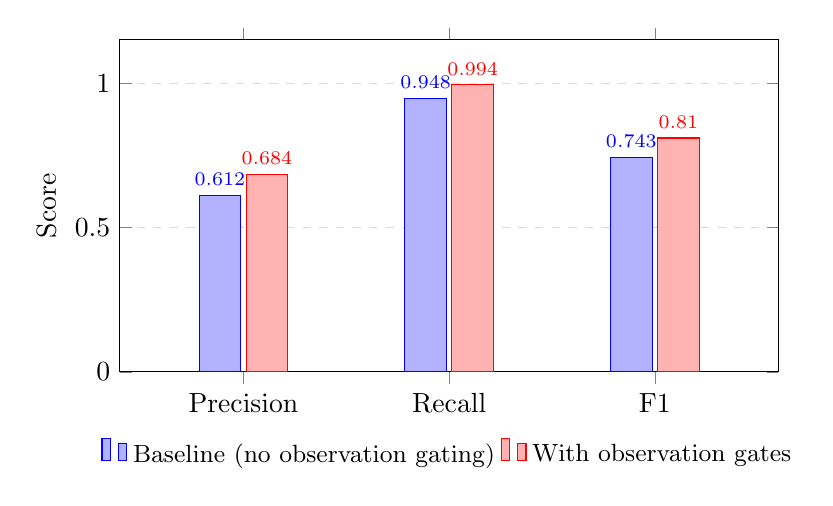
\begin{tikzpicture}
\begin{axis}[
    ybar,
    width=0.82\textwidth,
    height=58mm,
    bar width=15pt,
    ymin=0, ymax=1.15,
    ylabel={Score},
    symbolic x coords={Precision, Recall, F1},
    xtick=data,
    nodes near coords,
    nodes near coords style={font=\scriptsize, /pgf/number format/fixed,
                             /pgf/number format/precision=3},
    legend style={at={(0.5,-0.18)}, anchor=north, legend columns=2, font=\small,
                  draw=none},
    enlarge x limits=0.3,
    ymajorgrids=true,
    grid style={dashed, gray!30},
]
\addplot coordinates {(Precision,0.612) (Recall,0.948) (F1,0.743)};
\addplot coordinates {(Precision,0.684) (Recall,0.994) (F1,0.810)};
\legend{Baseline (no observation gating), With observation gates}
\end{axis}
\end{tikzpicture}
\caption{Observation-gate ablation. Gating raises precision without sacrificing recall,
yielding the net $F_1$ gain.}
\label{fig:ablation}
\end{figure}

As Figure~\ref{fig:ablation} makes visible, observation gating raises $F_1$ by
$+0.067$ (from 0.743 to 0.810), driven by a
precision gain (numeric-precondition recommendations no longer fire for every CCD patient)
with recall essentially unchanged. Because both configurations
share the same baseline, the ablation isolates the contribution of observation gating
itself. What it does not isolate is the contribution of the container. Whether that gain
actually requires FHIR is a separate question, and it is tested on its own in
Section~\ref{sec:csv-gating}.

\subsection{Where the gain comes from}
\label{sec:ablation-class}
A single overall figure hides more than it shows, because most of what it averages
cannot move at all. Section~\ref{sec:disc-class} sorts the 68 non-contraindication
recommendations by how each one can narrow the cohort, and only the 15 that carry a numeric
precondition are scored any differently with gating switched on. The other 53 give the same
answer either way, so they dilute the average without contributing to the change it is meant
to show. Table~\ref{tab:ablation-class} therefore reports concordance for each class
separately, in both arms.

\begin{table}[h]
\centering
\caption{Concordance by discrimination class in both ablation arms, micro-averaged over
the 876-patient cohort. Classes are those of Section~\ref{sec:disc-class}:
\emph{universal} recommendations carry no mechanism for narrowing the cohort at all,
\emph{concept-matched} require a further condition target, \emph{value-gated} a numeric
predicate over an observation, and \emph{both} require the two together. The two ungated
classes are identical in both arms to the individual count; the entire ablation effect is
confined to the 15 gated recommendations.}
\label{tab:ablation-class}
\footnotesize
\setlength{\tabcolsep}{4pt}
\begin{tabular}{lr|ccc|ccc}
\hline
& & \multicolumn{3}{c|}{\textbf{Baseline (no gating)}}
  & \multicolumn{3}{c}{\textbf{With observation gates}} \\
\textbf{Class} & \textbf{recs} & \textbf{P} & \textbf{R} & \textbf{$F_1$}
                               & \textbf{P} & \textbf{R} & \textbf{$F_1$} \\
\hline
Universal        & 38 & 0.666 & 1.000 & 0.799 & 0.666 & 1.000 & 0.799 \\
Concept-matched  & 15 & 0.676 & 0.915 & 0.777 & 0.676 & 0.915 & 0.777 \\
Value-gated      & \phantom{0}5 & 0.194 & 1.000 & 0.325
                                & \textbf{1.000} & \textbf{1.000} & \textbf{1.000} \\
Both             & 10 & 0.038 & 0.006 & 0.011
                                & \textbf{1.000} & \textbf{1.000} & \textbf{1.000} \\
\hline
\textbf{All}     & 68 & 0.613 & 0.945 & 0.743 & 0.685 & 0.993 & 0.811 \\
\hline
\end{tabular}
\end{table}

Four results follow from Table~\ref{tab:ablation-class}.

First, the two ungated classes are \emph{identical} across the arms---not merely close, but
equal to the individual true-positive, false-positive and false-negative count
($22{,}158/11{,}130/0$ for universal, $2{,}018/969/188$ for concept-matched). Fifty-three of
the 68 recommendations are therefore untouched, and the whole of the reported $F_1$
difference originates in the remaining 15. This is a falsifiable prediction of the
classification in Section~\ref{sec:disc-class}, and it holds exactly.

Second, the two gated classes benefit in opposite ways. For the \emph{value-gated} five, gating is a \emph{precision} mechanism: without it they
fire for every cohort member (849 true positives against 3{,}531 false positives,
$P = 0.194$), and with it they fire only where the measured value satisfies the predicate
($P = 1.000$) while recall was already perfect. For the \emph{both} class, gating is overwhelmingly a \emph{recall} mechanism. In the
baseline arm these ten recommendations almost never fire at all (8 true positives against
1{,}263 false negatives, $R = 0.006$), because their encoded condition targets alone rarely
match. The observation predicate is what actually identifies the patients they apply to. Describing the ablation solely as a
precision improvement is therefore incorrect for two thirds of the affected
recommendations.

Third, both gated classes reach $P = R = 1.000$ once gating is switched on. That
perfect score says something about the plumbing, not about how hard the clinical judgement is.
The observation gate and the reference standard apply the same guideline thresholds, such as
an ejection fraction at or below 40\%. They read the patient's value from different places,
however. The gate reads it from the graph, and the reference standard from the raw FHIR
bundle. Agreeing on every patient therefore shows that the loader carried those values across
without altering them. It does not show that the thresholds are clinically right, because both
sides were given the same thresholds to start with. Section~\ref{sec:shared-predicate}
establishes that the two are in fact the same function, then measures how much of the
concordance figure rests on that.

Fourth, five of the ten \emph{both}-class recommendations are \emph{inert}. \texttt{TP:2},
\texttt{TP:3:1}, \texttt{TP:3:2}, \texttt{TP:4} and \texttt{TP:5} record zero true positives,
zero false positives and zero false negatives in \emph{both} arms, and so contribute nothing to
either column. All five gate on a single predicate---current daily smoking---which no patient in
the cohort satisfies: of the 876, 390 are recorded as never having
smoked, 237 as ex-smokers, 249 carry no smoking observation at all,
and 0 are current smokers. The \emph{both} row is therefore driven entirely by five
active recommendations, and the counts quoted above belong to those five rather than to ten.
\texttt{LIPID:9} is inert for the same kind of reason---no cohort patient meets its
conjunction---so the gate it acquired when triglycerides were loaded is never exercised.

This generalises beyond the gated classes. 22 of the 73 recommendation
identifiers in the reference-label file have no positive instance anywhere in the cohort. That is
a property of the synthetic population rather than of the encoding: the recommendations are
encoded correctly and would fire given the relevant patients. It nonetheless bounds what these
concordance figures can demonstrate, and a real cohort would exercise a different and probably
larger subset. Section~\ref{sec:module-yield} identifies the principal cause. Of the 876 patients, 249,
some 28\%, come from the disease-enriched Synthea run. Their records carry only an
ischemic-heart-disease diagnosis, an abnormal cardiac imaging finding and sometimes a bypass
history, with no comorbidity and, apart from ejection fraction, no observation at all.

One choice of averaging runs through the whole table. The figures are \emph{micro}-averaged: every true positive, false positive and false
negative in the cohort is added up first, and the ratios are computed once at the end.

The other option, \emph{macro}-averaging, scores each patient on their own and then averages
those scores. It does not work here. A patient may not be touched by a class at all. There is then nothing for the system to get
right and nothing for it to get wrong, so all three counts are zero. Precision, recall and
$F_1$ are set to zero in that case, rather than left blank. That zero
goes into the average as though the system had failed the patient. The rarer the class, the
more such patients there are, and the further its macro figure sinks. What the number ends up
measuring is how common the class is, not how well the system handled it.

The value-gated class shows this at full size: macro $F_1 = 0.600$ against a micro value of
$1.000$. The two do not contradict each other. Because that class has no false positive and no
false negative anywhere, every patient scores either exactly one or exactly zero, so the macro
figure is simply the fraction of the cohort carrying a value-gated recommendation at all---526
of the 876. Every patient the class does apply to is scored perfectly. That is why every
per-class figure reported here is micro-averaged.

\subsection{Which part an independent judge scored}
\label{sec:shared-predicate}
Section~\ref{sec:oracle} separates the reference standard's independence into two tiers. This
section reports what that does to the figures.

For the 15 observation-gated recommendations, the system's predicate and the reference
standard's rule are the same function. This was checked empirically rather than read off the
source: both sides were evaluated on the 876 real cohort feature vectors and on 200{,}000
synthetic vectors aimed at every threshold they test, missing values included, and not one of
the 200{,}876 comparisons differed. Precision and recall of $1.000$ in the two gated classes
therefore cannot be read as a verdict on whether the rule is right.

Table~\ref{tab:shared-predicate} separates the two.

\begin{table}[h]
\centering
\caption{Guideline concordance split by the tier of independence of its reference standard,
micro-averaged over the 876-patient cohort.}
\label{tab:shared-predicate}
\begin{tabular}{lrcccrrr}
\hline
\textbf{Subset} & \textbf{recs} & \textbf{Precision} & \textbf{Recall} & \textbf{$F_1$} &
\textbf{tp} & \textbf{fp} & \textbf{fn} \\
\hline
All                & 68 & 0.685 & 0.993 & 0.811 & 26{,}296 & 12{,}099 & 188 \\
Shared predicate   & 15 & 1.000 & 1.000 & 1.000 & 2{,}120 & 0 & 0 \\
Independent logic  & 53 & 0.666 & 0.992 & 0.797 & 24{,}176 & 12{,}099 & 188 \\
\hline
\end{tabular}
\end{table}

The part scored by a genuinely independent judge covers 53 of the 68 recommendations and reaches
precision $0.666$ and $F_1$ $0.797$. Removing the fifteen shared-predicate recommendations
therefore costs $0.018$ of precision and $0.013$ of $F_1$; $8.1\%$ of all true positives come
from the shared-predicate part. The headline figure is not propped up by the shared part, and
the concordance conclusion survives deleting that part entirely.

The ablation is a different matter, and should be stated frankly. Only the value-gated and both
classes change between the ablation arms, and those are exactly the fifteen shared-predicate
recommendations. The whole of the ablation gain is therefore measured on recommendations whose
reference standard applies the same rule as the system. The gain is still a real change in the system's behaviour. Ungated, numeric-precondition
recommendations fire for patients who do not meet the precondition the guideline states, and
that is a defect whoever judges it. What the gain measures, though, is implementation
fidelity, not clinical validity. The reference standard is an
independent judge of the values fed to the rule, not of the rule.

\subsection{Does the gain require FHIR?}
\label{sec:csv-gating}
The ablation in Table~\ref{tab:ablation} isolates the contribution of observation gating, not
the contribution of the container. The two are easily conflated. Chapter~I motivates the
FHIR-native design by contrast with flattened tabular exports, from which it is a short step to
concluding that the gate is possible \emph{because of} FHIR. That conclusion was asserted rather
than measured. This section measures it.

The test is a third arm. The same gate was rebuilt reading only Synthea's CSV
export---\texttt{observations.csv} and \texttt{conditions.csv}---touching neither the bundles nor
the graph. The string-matching logic, the thresholds and the aggregation rules were copied
verbatim from \texttt{silver\_oracle.py}, so that any disagreement would be attributable to the
container and not to a difference in clinical logic. That is the point of the design.

The comparison target is the FHIR bundle path, not the graph path. For this purpose they are the
same thing: the fifteen observation-gated recommendations score precision and recall of $1.000$
against the reference standard across the whole cohort, as reported in
Section~\ref{sec:ablation-class}, so the graph's gate decisions and the reference standard's
already agree everywhere. Reproducing the reference standard therefore reproduces the graph gate
too, without needing Neo4j.

Table~\ref{tab:csv-gating} reports the result.

\begin{table}[h]
\centering
\caption{The observation gate built from the FHIR bundles against the same gate built from the
CSV export, for the 15 observation-gated recommendations across 876 patients.}
\label{tab:csv-gating}
\begin{tabular}{lcccrrr}
\hline
\textbf{Source} & \textbf{Precision} & \textbf{Recall} & \textbf{$F_1$} &
\textbf{tp} & \textbf{fp} & \textbf{fn} \\
\hline
FHIR bundles & 1.000 & 1.000 & 1.000 & 2{,}120 & 0 & 0 \\
CSV export   & 1.000 & 1.000 & 1.000 & 2{,}120 & 0 & 0 \\
\hline
\end{tabular}
\end{table}

Of 13{,}140 gate decisions---876 patients times 15 recommendations---not one differs between the
two sources. The count of 2{,}120 is itself the sum of the true positives of the two gated
classes in the gated arm of Table~\ref{tab:ablation-class}---849 for value-gated and 1{,}271 for
both---so the agreement doubles as a check that the reconstruction measures the same thing. The
cohort fares likewise: SNOMED~CT code \texttt{414545008} in \texttt{conditions.csv} selects
exactly the same 876 patients as the graph's gate.

Two things the export genuinely loses can be measured, and neither changed a decision. First,
the export rounds observation values to one decimal place. That makes 1{,}990 values differ
between the two paths, by at most $0.05$. Three of them land on the far side of a threshold. One
ejection-fraction case ($39.999$ becoming $40.0$) is not exposure at all, because the predicates
that use it test ``$\le 40$'' and ``$> 40$'', which both values answer identically. Two triglyceride cases ($149.97$ and $149.96$, both becoming $150.0$) are real exposure,
because the clause ``$150 \le$ triglycerides'' flips to true. \texttt{LIPID:9}, however,
also requires LDL below 100, which fails for both patients ($130.1$ and $148.6$). No recommendation changed.

Second, the blood-pressure panel does not survive, exactly as Section~\ref{sec:flattening} states.
Recovering it, however, requires no guesswork. The \texttt{ENCOUNTER} column is populated on every
observation row, so the 17{,}177 systolic and diastolic pairs in this cohort reassemble completely,
leaving no row unpaired. The reassembly is a cost, not an obstacle.

The conclusion that follows is narrower than Chapter~I originally asserted. The precision gain is
real and unchanged: observation gating still raises $F_1$ by $+0.067$. What the evidence does not
support is attributing that gain to the FHIR container specifically. What produces it is loading
numeric observation values as first-class data. FHIR makes that direct; Synthea's tabular export
permits it too, at the price of one reassembly step and one decimal place of precision. The distinction matters because it sets what may be claimed. The claim is not that FHIR is
necessary, but that numeric observations are. FHIR is the most direct way to obtain them.

The scope of this conclusion should be stated plainly. What the test shows is that Synthea's CSV
export carries enough data for the nine LOINC codes this gate uses, on this corpus. It does not
show that CSV and FHIR are equivalent in general, and it does not extend to tabular exports from
other systems, which need not carry a foreign key such as \texttt{ENCOUNTER}. The things the
export does still lose---resource \texttt{status}, the code system on an observation value, and
the panel's identity as a unit---are discussed in Section~\ref{sec:flattening}; none is used by
this gate, but that is a property of this corpus rather than of the design.

\section{Silver-Standard Validation Against the Gold Standard}
\label{sec:gold}

To validate the automatically generated silver standard, 30 patients were
labelled manually to form the gold standard and compared against the silver labels.
Agreement was 99.5\% (2{,}150 of 2{,}160 cells) with Cohen's
$\kappa = 0.991$ (95\% confidence interval 0.984--0.996; Section~\ref{sec:kappa-ci}),
indicating near-perfect agreement. This is the result that
licenses the rest of the evaluation. Because the silver standard reproduces human
judgement almost exactly on the sample where both exist, the concordance figures computed
against it over the full 876-patient cohort rest on a validated reference
rather than an assumed one. That is the standard justification for substituting
automatically generated labels for manual annotation at scale
\cite{rebholz2011,nogues2022}. The annotator and the rubric are given in Section~\ref{sec:goldlabel}.

\subsection{The residual disagreements}
Ten of the 2{,}160 compared cells disagree. They are enumerated individually in
Table~\ref{tab:disagreements} rather than summarised, because their distribution is more
informative than their count.

\begin{table}[h]
\centering
\caption{All silver--gold disagreements. ``Over'' denotes the silver standard labelling a
recommendation applicable where the human did not; ``under'' the reverse.}
\label{tab:disagreements}
\footnotesize
\begin{tabular}{llccl}
\hline
\textbf{Patient} & \textbf{Recommendation} & \textbf{COR} & \textbf{Silver / Gold}
& \textbf{Direction} \\
\hline
\texttt{cbf432fc} & \texttt{APT:6}    & 2b & 1 / 0 & over  \\
\texttt{6595b70f} & \texttt{BB:2}     & 1  & 0 / 1 & under \\
\texttt{1db4196c} & \texttt{BPM:3}    & 1  & 1 / 0 & over  \\
\texttt{05e41fe3} & \texttt{LIPID:2}  & 1  & 1 / 0 & over  \\
\texttt{22f599b6} & \texttt{LIPID:2}  & 1  & 1 / 0 & over  \\
\texttt{2b050f16} & \texttt{LIPID:2}  & 1  & 0 / 1 & under \\
\texttt{2b050f16} & \texttt{LIPID:3}  & 1  & 1 / 0 & over  \\
\texttt{04287b67} & \texttt{LIPID:5}  & 2a & 0 / 1 & under \\
\texttt{cbf432fc} & \texttt{LIPID:5}  & 2a & 0 / 1 & under \\
\texttt{227e76d8} & \texttt{LIPID:10} & 2b & 0 / 1 & under \\
\hline
\end{tabular}
\end{table}

Three properties of this set matter. First, the disagreements are \emph{exactly balanced}:
five over-labels and five under-labels, against 1{,}080 cells where both mark the
recommendation applicable and 1{,}070 where both do not. The silver standard is therefore
not systematically more or less permissive than the human labeller, which is the property
that most threatens the use of an automated reference and the one hardest to establish by
argument alone.

Second, the disagreements are \emph{concentrated}, not scattered: seven of the ten concern
lipid recommendations (\texttt{LIPID:2} three times, \texttt{LIPID:5} twice,
\texttt{LIPID:3} and \texttt{LIPID:10} once each). This is where the guideline text is
least mechanisable. \texttt{LIPID:2} applies when high-intensity statin therapy is
``contraindicated or not tolerated''---intolerance is not represented in the coded record,
so both the silver standard and the human must infer it. \texttt{LIPID:5} applies to
patients ``judged to be at very high risk'', a composite the guideline explicitly leaves
to clinical judgement. \texttt{LIPID:10} requires simultaneously that the patient is
\emph{not} at very high risk, is on ``maximally tolerated'' statin therapy, and has
LDL-C~$\geq$~70~mg/dL. These are precisely the clauses the reference standard's
unconfirmable-clause policy (Section~\ref{sec:oracle}) abstains on. The residual error is
therefore localised to irreducibly judgemental preconditions rather than distributed
across the recommendation set, which is the more reassuring of the two possibilities.

Third, the ten cells represent \emph{fewer than ten independent judgements}. Patient
\texttt{2b050f16} accounts for two of them---an under-label on \texttt{LIPID:2} and an
over-label on \texttt{LIPID:3}---which together are most plausibly a single disagreement
about statin intensity recorded in two cells; patient \texttt{cbf432fc} likewise accounts
for two. Cohen's $\kappa$ treats every cell as independent, so the reported value slightly
\emph{understates} the true level of agreement.

\subsection{Uncertainty of $\kappa$ and whether 30 patients suffice}
\label{sec:kappa-ci}
The same dependence bears on the uncertainty of $\kappa$. The 2{,}160 compared cells are
clustered in 30 patients, and one patient's record determines all of that patient's labels at
once. The appropriate confidence interval therefore resamples \emph{patients}, not cells
(Section~\ref{sec:goldlabel}). Table~\ref{tab:kappa-ci} reports both, so the difference can be
seen.

\begin{table}[h]
\centering
\caption{95\% confidence intervals for the silver--gold Cohen's $\kappa$, from 10{,}000
bootstrap replicates for each resampling unit.}
\label{tab:kappa-ci}
\begin{tabular}{lcc}
\hline
\textbf{Resampling unit} & \textbf{Lower bound} & \textbf{Upper bound} \\
\hline
Cells, assuming independence & 0.984 & 0.996 \\
Patients (cluster bootstrap)  & 0.984 & 0.996 \\
\hline
\end{tabular}
\end{table}

Both give the same interval, 0.984 to 0.996. The reason is how the disagreements are spread.
The ten disagreements fall on 8 of the 30 patients, and no patient contributes more than two.
The design effect is only 1.04, so clustering by patient adds almost no uncertainty. A
jackknife that drops one patient at a time gives $\kappa$ between 0.990 and 0.992. No single
patient, therefore, is holding the figure up.

Nor is $\kappa$ inflated by label prevalence. Positive labels cover 1{,}085 of 2{,}160 cells in
both standards (50.2\%), the prevalence index is 0.005, and the bias index is zero because the
disagreements split five and five. Chance agreement is therefore about 0.500, and $\kappa$ is
practically equal to PABAK, at 0.991 \cite{byrt1993}.

Whether 30 patients suffice depends on the claim being supported. For the claim that the silver
standard agrees near-perfectly with manual labelling, 30 patients are enough. The lower bound of
the interval, 0.984, is well above the 0.80 threshold \cite{landis1977}, and none of the 10{,}000
replicates falls below 0.95. For a finer claim, such as that $\kappa$ is 0.99 rather than 0.98,
30 patients are not enough, and no such claim is made.

The interval has two bounds. First, it describes only patients like these thirty, who were
chosen purposively and lean towards the most complex records (Section~\ref{sec:gate}). Second,
it does not address the single-annotator limitation, since resampling cannot produce a second
rater (Section~\ref{sec:limitations}).

\section{Safety Detection}
\label{sec:safety-detection}

Contraindication-safety detection was evaluated on the 151 manually labelled
safety flags (Table~\ref{tab:safety}).

\begin{table}[h]
\centering
\caption{Contraindication-safety detection: unary vs.\ population-gated matching.}
\label{tab:safety}
\begin{tabular}{lccc}
\hline
\textbf{Variant} & \textbf{Precision} & \textbf{Recall} & \textbf{$F_1$} \\
\hline
Unary (on the contraindicated drug) & 0.139 & $\approx$1.000 & --- \\
Population-gated (drug \emph{and} population condition) & 1.000 & 0.095 & 0.174 \\
\hline
\end{tabular}
\end{table}

The result exposes a genuine trade-off rather than a tunable failure: unary matching never
misses a reachable contraindication but over-flags heavily, whereas population gating is
perfectly precise but recovers only the minority of contraindications whose population
condition is structurally gateable; the misses are the negation-defined and conjunctive
contraindications that a flat schema cannot express.

Beyond this binary trade-off, the chronic-NSAID recommendation (\texttt{APT:10}) was scored
under a third, \emph{chronicity-gated} variant that fires only when the graph judges the
NSAID use chronic from the categorical medication status and the recurring-course count.
Against the manually labelled flags this variant reached precision 0.909 and
recall 0.526 (tp $=10$, fp $=1$, fn $=9$)---highly precise, but
recovering only about half of the truly chronic cases. The missed cases are precisely those that are chronic \emph{only} through a single long
course, for example a 101-day and a 111-day ibuprofen prescription. The graph cannot see
such cases because the FHIR export lacks stop dates (Section~\ref{sec:chronicity}). This is
not a tuning artefact but a measured price of the FHIR-native design: the categorical
medication status recovers the ongoing and multi-course arms of the chronicity rule, but the
duration arms are structurally unrecoverable from FHIR alone.

\section{Briefing Faithfulness}
\label{sec:faithfulness}

The grounded briefing was generated for 30 patients, the same sample as the gold standard,
and checked automatically against the retrieved facts. Five of them were generated first and
formed the basis of this work's initial report. The other twenty-five were generated later
with the same pipeline and model.

The check tests four things. First, every recommendation identifier the briefing cites must
be in the facts. Second, every PMID it cites must be in the facts too. Third, every
applicable recommendation and every safety flag in the facts must be mentioned. Fourth, the
briefing must not state that the patient requires oral anticoagulation when no anticoagulant
is on the medication list. A conditional statement such as ``if requiring oral
anticoagulation'' is still allowed.

All 30 briefings pass all four tests: zero fabricated recommendations, zero fabricated PMIDs,
zero omitted recommendations, and zero anticoagulation over-claims.

The fourth test needs to be reported with its history. On its first run over the 30
briefings, it flagged 10 lines in 4 briefings as over-claims. All 10 turned out to be false
positives of the same shape. The briefing's provenance trace wrote ``conditional on oral
anticoagulation need (not confirmed in current medications)'', and the pattern matched the
word \emph{on} inside \emph{conditional on}. The test was then restricted to the parts of the
briefing a reader acts on. Mentions in the provenance trace are still counted and reported,
not discarded. That correction was made \emph{after} the output was seen, and it should be
stated. The five-of-five result in the initial report held partly because the first five
briefings happened to phrase their conditional statements in a form the check recognised.

These four tests are not the same as semantic faithfulness. Deterministic retrieval
guarantees that the facts the language model receives are exact and reproducible. It also
makes citable items checkable against a closed set of facts. It does not, however, guarantee
that every sentence the model writes is faithful to those facts. The model can still, for
example, attach to the patient a condition or drug that is not in the facts, misstate why a
recommendation applies, or present a weak-class recommendation as if it were mandatory.
Apart from the anticoagulation pattern, none of these errors is caught by this check. What is
reported here is therefore citation-level and completeness faithfulness, plus one over-claim
pattern. The semantic faithfulness of every sentence still requires a human reading, and it
is recorded as a limitation in Section~\ref{sec:limitations}.

The briefing's safety tier applies the same graph-only chronicity gate as the recommendation
layer. For patients whose NSAID use is chronic \emph{only} by duration, the chronic-NSAID flag
is therefore withheld rather than asserted without support. That omission is consistent with
the safety-detection recall reported in Section~\ref{sec:safety-detection}, and traceable to
it.

Appendix~\ref{app:briefing} reproduces one briefing in full, unedited, so that what the check actually inspects can be read directly rather than described.

\section{Clinician Review}
\label{sec:clinician}

This section reports clinicians' judgements of the appropriateness of the recommendations the
system outputs (Section~\ref{sec:clinician-method}). Table~\ref{tab:clinician} summarises the
ratings by rater and by recommendation type. Antithrombotic recommendations cover
antiplatelet and anticoagulant therapy (\texttt{APT}); beta-blocker recommendations cover the
review of long-term use and the beta-blocker check/stop flags (\texttt{BB}).

\begin{table}[h]
\centering
\caption{Clinician ratings by rater and recommendation type. Percentages are of the rows that
rater rated.}
\label{tab:clinician}
\small
\begin{tabular}{llrrrr}
\hline
\textbf{Rater} & \textbf{Recommendations} & \textbf{Rows} & \textbf{Appropriate} &
\begin{tabular}[b]{@{}r@{}}\textbf{Not yet}\\\textbf{appropriate}\end{tabular} &
\begin{tabular}[b]{@{}r@{}}\textbf{Cannot be}\\\textbf{judged}\end{tabular} \\
\hline
A (cardiologist)  & Antithrombotic & 101 & 52  & 46 & 3  \\
                  & Beta blocker   & 40  & 35  & 5  & 0  \\
                  & Other          & 106 & 105 & 1  & 0  \\
                  & All            & 247 & 192 (77.7\%) & 52 (21.1\%) & 3 (1.2\%) \\
\hline
B (GP)            & Antithrombotic & 66  & 19  & 32 & 15 \\
                  & Beta blocker   & 25  & 9   & 1  & 15 \\
                  & Other          & 69  & 69  & 0  & 0  \\
                  & All            & 160 & 97 (60.6\%) & 33 (20.6\%) & 30 (18.8\%) \\
\hline
C (senior cardiologist) & All      & 16  & 6   & 5  & 5  \\
\hline
\end{tabular}
\end{table}

Rater~A judged 192 of 247 recommendations appropriate (77.7\%; 95\% per-patient confidence
interval 74.4--81.1\%). Rater~B judged 97 of 160 appropriate (60.6\%; 56.1--67.3\%). The
difference comes mostly from ``cannot be judged'', which rater~B chose on 30 rows and
rater~A on 3. Excluding those rows, the two proportions are closer, at 78.7\% and 74.6\%.

Judgements of inappropriateness concentrate on antithrombotic recommendations. Of the
``not yet appropriate'' ratings, 46 of rater~A's 52 and 32 of rater~B's 33 fall on them.
Outside the antithrombotic and beta-blocker recommendations, by contrast, rater~A judged 105
of 106 rows appropriate and rater~B all 69. That group covers the blood-pressure target and
first-line antihypertensives, cardiac-rehabilitation referral, weight management, SGLT2
inhibitors, and the safety flag for nitrates with a PDE5 inhibitor. It also includes three
shared-predicate recommendations (Section~\ref{sec:shared-predicate}): \texttt{WM:2},
\texttt{WM:3}, and \texttt{SGLT2:4}. All three were judged appropriate on all 30 of rater~A's
rows and all 20 of rater~B's. For those three, the clinicians' judgement provides a test of
the rule that the reference standard cannot.

Raters~A and~B both rated 159 rows across 10 patients. Their observed agreement is 65.4\%
(95\% per-patient confidence interval 58.8--73.9\%), with Cohen's $\kappa = 0.29$
(0.18--0.41) and PABAK 0.48. A $\kappa$ of that size is fair agreement \cite{landis1977}. The
agreement is uneven. On the 69 rows outside the antithrombotic and beta-blocker
recommendations, they agree on 68 (98.6\%). On the 90 antithrombotic and beta-blocker rows,
they agree on only 36 (40.0\%). Of the 55 disagreements, 27 involve rater~B's ``cannot be
judged''.

The raters' comments show where the disagreement comes from. Rater~A wrote none. Almost every
``cannot be judged'' from rater~B asks for information the conclusion did not show: ejection
fraction and heart-failure status for the beta-blocker recommendations, and bleeding risk for
extending dual antiplatelet therapy and for adding vorapaxar. On the three conditional
anticoagulant recommendations (\texttt{APT:11}--\texttt{APT:13}), rater~B chose ``not yet
appropriate'' on 23 of 24 rows. In their place, rater~B proposed a different sequence: triple therapy for one
week, then a DOAC with clopidogrel for up to one year, then a DOAC long term. Rater~A judged 13
of 15 clopidogrel check/stop flags (\texttt{APT:7}) not yet appropriate, and rater~B 5 of 11.
Rater~B's comments on those rows reject stopping clopidogrel: a post-infarction patient still
needs dual antiplatelet therapy, or clopidogrel alone if bleeding risk is high.

Rater~C judged 6 of the 16 recommendations for patient~1 appropriate. The comments expose a
limit of the review sheet. Rater~C chose ``cannot be judged'' for two check/stop flags,
clopidogrel and nitroglycerin, because neither drug appears in the conclusion, although both
are in the patient's record. The same option was given to the three conditional
anticoagulant recommendations, because the patient has no indication for anticoagulation.
Both beta-blocker check/stop flags were judged not yet appropriate, because in rater~C's view
the patient needs a beta blocker. On patient~1, rater~C agrees with rater~A on 6 of 16 rows
and with rater~B also on 6; all three agree on 5.

Overall, the clinicians judged most of the system's recommendations appropriate for their
patients. Rater~A, the cardiologist who rated the most patients (15), judged 77.7\%
appropriate. For rater~B, a general practitioner, the proportion judged appropriate is lower,
because more of rater~B's rows were marked ``cannot be judged''. Almost every recommendation
outside antithrombotic and beta-blocker therapy was judged appropriate, with high agreement
between the raters. By contrast, most ``not yet appropriate'' ratings fall on the
antithrombotic recommendations. On the beta-blocker recommendations, almost all the
disagreement between raters comes from ``cannot be judged''. Rater~B added that information
on ejection fraction and heart-failure status is needed for those recommendations to be
judged. The antithrombotic and beta-blocker recommendations therefore show a common pattern
in the ratings: they depend on information the system's conclusion did not present, such as
time since an acute coronary syndrome, bleeding risk, the indication for anticoagulation,
ejection fraction, and heart-failure status. The review thus shows that clinicians generally
judge the system's recommendations appropriate. It also identifies what to improve first: the
antithrombotic and beta-blocker recommendations, with an explanation of the information they
rest on.

\section{Comparison with Prior Work}
\label{sec:prior-work}

This section positions the results against previously published systems.
Table~\ref{tab:prior-systems} compares along the five dimensions that distinguish this
work: the data source, whether terminologies are bridged into a common concept space,
whether a clinical guideline is encoded as a queryable layer, whether the output is
evaluated against an independent reference, and whether generated text is mechanically
checked for faithfulness.

\begin{table}[h]
\centering
\caption{Comparison with prior knowledge-graph and FHIR-based clinical decision support.}
\label{tab:prior-systems}
\footnotesize
\setlength{\tabcolsep}{3pt}
\begin{tabular}{p{22mm}p{20mm}p{18mm}p{18mm}p{24mm}p{16mm}}
\hline
\textbf{Work} & \textbf{Data source} & \textbf{Concept bridge} & \textbf{Guideline layer}
& \textbf{Evaluated vs.\ reference} & \textbf{Faithful. checked} \\
\hline
This work
  & Synthetic FHIR R4 (Synthea)
  & UMLS CUI
  & 2023 AHA/ACC CCD, 81 recs
  & Independent oracle + manual gold ($\kappa$)
  & Yes, automated \\
Zhou \textit{et al.} \cite{zhou2022}
  & 124 records, one physician
  & Not reported
  & Chinese hypertension guideline
  & Ranking (recall, hit@3, MRR)
  & N/A (no text) \\
Semenov \textit{et al.} \cite{semenov2018}
  & FHIR engine, lab results
  & LOINC only
  & Production rules
  & Not reported
  & No \\
Xiao \textit{et al.} \cite{xiao2022}
  & OMOP CDM / MIMIC-III $\rightarrow$ FHIR RDF
  & OMOP vocab.
  & None
  & Query-equiv.\ + spec conformance
  & N/A (no text) \\
Cui \textit{et al.} \cite{cui2025}
  & Guideline text only
  & Ontology
  & Cardiovascular medication guides
  & Expert iterative review
  & N/A (no text) \\
Ehtesham \textit{et al.} \cite{ehtesham2025}
  & Synthetic FHIR R4 (SMART)
  & No
  & None
  & Not reported
  & No \\
Sudri \textit{et al.} \cite{sudri2024}
  & Angiography case notes
  & No
  & Implicit in model
  & Heart team, $\kappa = 0.59$
  & No \\
\hline
\end{tabular}

\vspace{2pt}
\end{table}

The closest system in capability is that of Zhou \textit{et al.}~\cite{zhou2022}, which
likewise couples a guideline-derived graph to patient records and evaluates the
recommendations it produces; Section~\ref{sec:rw-kg} sets out what separates the two.
The closest \emph{architectural} comparable is the FHIR-based patient decision aid of Semenov
\textit{et al.}~\cite{semenov2018}, which likewise pairs a FHIR interoperability layer with
a graph-structured knowledge base. It is, however, a production-rule system
over laboratory results, with a knowledge base of 365 test-component nodes,
5{,}084 rule nodes, and 49{,}932 connections. The graph
reported here is larger by more than two orders of magnitude in both nodes
(1{,}804{,}379 against roughly $5.4\times10^{3}$) and relationships
(8{,}796{,}425 against $4.99\times10^{4}$). The difference is one of
\emph{scope}, not of merit: that system encodes rules over a narrow laboratory panel,
whereas this one ingests entire longitudinal patient records.

On graph construction, Xiao \textit{et al.}~\cite{xiao2022} is the closest prior effort in
methodological rigour, exposing an OMOP repository as FHIR RDF and validating it by
query equivalence against the source database. Their MIMIC-III derived graph
is larger in patient count (46{,}520 patients against 5{,}490 here) because
it draws on a real intensive care corpus. Crucially, that work appears to stop
at the clinical graph: it reports no guideline layer and issues no
recommendations, so no concordance evaluation is possible. Conversely, Cui
\textit{et al.}~\cite{cui2025} build a cardiovascular medication guideline graph---also in
Neo4j, with 22{,}475 medication entities and 3{,}304
relationships---but with no patient records attached, so it supports
knowledge retrieval rather than patient-specific decision support. The contribution here is
precisely the join these two leave open: patient records and guideline recommendations in
one graph, bridged through shared concepts, with the patient-to-recommendation traversal
evaluated end-to-end. A related knowledge-graph analysis of stress echocardiography in
coronary disease~\cite{wu2023} is domain-adjacent but appears to be
a literature-mining study rather than a patient-facing system.

Two comparisons concern the language-model tier. Ehtesham \textit{et al.}~\cite{ehtesham2025}
also drive an LLM over synthetic FHIR records, but retrieval is agent-directed
rather than deterministic, and no faithfulness verification is reported---the property this
work treats as central. Sudri \textit{et al.}~\cite{sudri2024} work in the same clinical
territory (coronary revascularization) and report that an ungrounded GPT-4 reaches accuracy
0.82 and $\kappa = 0.59$ against a multidisciplinary heart
team, with GPT-3.5 at $\kappa = 0.12$.
\textbf{That figure is not directly comparable to the $\kappa = 0.991$ reported
in Section~\ref{sec:gold}}: theirs measures a language model's clinical judgement against
expert clinicians, whereas the value here measures an automated oracle against manual gold
labels. The relevant contrast is architectural rather than numerical---it indicates the
level of agreement obtainable when a model is asked to reason clinically without grounding,
which is the design this work deliberately avoids.

\subsection{Faithfulness in context}

The faithfulness result is best read against the framework of Asgari
\textit{et al.}~\cite{asgari2025}, who annotated 12{,}999 clinician-reviewed
sentences from LLM-generated clinical notes and measured a 1.47\%
hallucination rate and a 3.45\% omission rate
(Table~\ref{tab:faithful-compare}).

\begin{table}[h]
\centering
\caption{Faithfulness of generated clinical text: this work in context.}
\label{tab:faithful-compare}
\footnotesize
\begin{tabular}{lccl}
\hline
\textbf{Study} & \textbf{Fabrication} & \textbf{Omission} & \textbf{Evaluation sample} \\
\hline
Asgari \textit{et al.} \cite{asgari2025}
  & 1.47\% & 3.45\%
  & 12{,}999 clinician-annotated sentences \\
This work
  & 0 & 0
  & 30 briefings, all cited items checked \\
\hline
\end{tabular}

\vspace{2pt}
\end{table}

The two differ widely in both unit and sample size: clinician-annotated sentences against
automatically checked briefings. They therefore cannot be set side by side directly. The
correct statement about the briefings produced here is that \emph{no} fabrication or omission
was observed across 30 briefings whose cited items were all checked---not that this system
has a lower hallucination rate than the published benchmark. What the comparison does support is a claim about mechanism. Asgari
\textit{et al.} reduce errors by refining prompts and workflows, leaving a non-zero residual
because the model is still composing content. Here new citable content cannot get through
undetected: every citable item in the briefing must correspond to a retrieved fact, and the
check is decidable precisely because retrieval is deterministic. The residual risk therefore
shifts from fabrication to \emph{phrasing}. The over-claim check reaches only one pattern of
that risk (Section~\ref{sec:faithfulness}). Finally, the reader-study protocol of Van Veen \textit{et al.}~\cite{vanveen2023} had
physicians score summaries for completeness, correctness, and conciseness. That evaluation
is not performed in this work, since the clinician review of Section~\ref{sec:clinician}
judges the appropriateness of recommendations, not the quality of the summary. Faithfulness here is established against the record rather
than against a clinician's judgement, and closing that gap is the reader study proposed in
Section~\ref{sec:limitations}.

\section{Discussion}

Taken together, the results support the three research questions. First, a FHIR-native
knowledge graph fusing EHR, guideline, and literature was constructed and shown to be rich,
broad, and deeply connected. Second, loading numeric observations as first-class data
improved guideline concordance by $+0.067$ $F_1$ without loss of recall. FHIR supplies those
observations most directly, but not uniquely, since a tabular export reproduces the same gate
(Section~\ref{sec:csv-gating}). Third, all 30 grounded briefings passed the automated
faithfulness check. Because retrieval is deterministic, citable items can be checked against a
closed set of facts, which similarity-based retrieval-augmented generation cannot offer. That
advantage concerns citation-level faithfulness, not a guarantee that every sentence is
semantically faithful (Section~\ref{sec:faithfulness}). As
Section~\ref{sec:prior-work} sets out, prior FHIR-based graphs stop short of a guideline
layer \cite{xiao2022} while prior guideline graphs carry no patient records
\cite{cui2025}; joining the two and evaluating the join end-to-end is where this work sits.

The residual errors are honest and instructive. Guideline preconditions that structured
data cannot confirm (composite risk scores, some negation-defined clauses) remain sources of
false positives, and the safety tier makes the unary-vs-gated trade-off explicit. The
clinician review points to the same place from another direction. Outside the antithrombotic
and beta-blocker recommendations, clinicians judged almost every recommendation appropriate.
The ratings of inappropriateness, and the disagreement between raters, concentrate on
recommendations whose guideline logic depends on information outside the conclusion: time
since an acute coronary syndrome, bleeding risk, the indication for anticoagulation, ejection
fraction, and heart-failure status (Section~\ref{sec:clinician}). Some of that information,
such as bleeding risk, is a composite score that structured data cannot confirm. Some, such
as the medication list, is in the record but was not presented in the conclusion the
clinicians read. A further finding concerns interoperability. The synthetic FHIR export is SNOMED-native and, unlike the
paired CSV export, omits medication stop dates while retaining a categorical medication
status; the CSV, conversely, retains stop dates but carries no status. Neither projection is
a superset of the other, so the graph-side chronicity gate can reconstruct only two of the
four arms of the chronic-use rule (Section~\ref{sec:chronicity}). The cost of this loss is
measured, not hypothetical: the chronicity-gated safety variant recovers only
53\% of truly chronic NSAID courses (Section~\ref{sec:safety-detection}), and the
corresponding briefing flag is honestly withheld for the two patients whose chronicity is
duration-only. A real deployment that consumes only FHIR must anticipate this class of
information loss and, where a guideline depends on exposure duration, recover it from an
auxiliary source.

\cleardoublepage \phantomsection
\chapter{Conclusions and Future Work}

\section{Conclusions}

This thesis set out to build a FHIR-native, knowledge-graph-based clinical recommendation
system for chronic coronary disease, and to establish by measurement what the FHIR-native
design actually buys. The system was built, and each of the three research objectives stated
in Chapter~I can now be answered from the results of Chapter~IV.

\begin{enumerate}
    \item \textbf{The pipeline was realised and evaluated end to end.} HL7 FHIR~R4 bundles
    for 5{,}490 patients were loaded into a Neo4j property graph and fused with the 2023
    AHA/ACC CCD guideline and a guideline-seeded literature corpus through a UMLS concept
    bridge, yielding a graph of 1{,}804{,}379 nodes and 8{,}796{,}425 relationships over 25
    labels, 51 relationship types and 26 code systems
    (Section~\ref{sec:kg-results}). The \texttt{:Patient} count equals the number of patients
    Synthea reported generating, so the idempotent load neither dropped nor duplicated a
    record. Against a reference standard generated over a data path separate from the system's,
    guideline concordance over the 876-patient evaluation cohort reached
    $F_1 = 0.810$ (Section~\ref{sec:ablation}); with the 15 recommendations whose predicate
    both sides share removed, the remaining 53 reach $F_1 = 0.797$
    (Section~\ref{sec:shared-predicate}). That figure rests on a
    validated reference rather than an assumed one: on the 30 patients labelled
    manually, the automated standard agrees on 99.5\% of cells
    (2{,}150 of 2{,}160) with Cohen's $\kappa = 0.991$ (95\% confidence interval
    0.984--0.996, resampling patients; Section~\ref{sec:kappa-ci}). Thirty patients are enough
    to support the claim of near-perfect agreement, but they were labelled by a single annotator
    (Section~\ref{sec:limitations}). The clinician review adds a judgement the reference
    standard cannot give: a cardiologist judged 77.7\% of 247 recommendations for 15 patients
    appropriate (Section~\ref{sec:clinician}). Outside the antithrombotic and beta-blocker
    recommendations, almost every recommendation was judged appropriate. The ratings of
    inappropriateness and the disagreement between raters ($\kappa = 0.29$) concentrate on
    antithrombotic recommendations, whose guideline logic depends on time since an acute
    coronary syndrome, bleeding risk, and the indication for anticoagulation. Objective~1 is
    therefore met.

    \item \textbf{Observation gating improves guideline concordance, and the ablation
    localises the improvement exactly.} Gating observation-dependent recommendations on the
    patient's measured values raises $F_1$ from 0.743 to
    0.810, a gain of $+0.067$ obtained through precision
    (0.612 to 0.684) with recall essentially unchanged
    (Section~\ref{sec:ablation}). The classification of Section~\ref{sec:disc-class} makes a
    falsifiable prediction about where that gain must live, and it holds exactly: 53 of the
    68 recommendations are identical in both arms down to the individual true-positive,
    false-positive and false-negative counts, and the whole of the difference originates in
    the 15 that are gated. A second and less obvious result is that gating is not one
    mechanism but two. For the five \emph{value-gated} recommendations it acts on precision, which rises from 0.194
    to 1.000 because they no longer fire for every cohort member. For the ten in the
    \emph{both} class it acts overwhelmingly on recall, which rises from 0.006 to 1.000.
    Their encoded condition targets alone rarely match, so it is the numeric predicate that
    identifies the patients they apply to (Section~\ref{sec:ablation-class}). Describing the ablation solely as a precision
    improvement, as the aggregate invites, is therefore wrong for two thirds of the affected
    recommendations. One qualification attaches to the ablation as a whole. The fifteen gated recommendations are
    precisely those whose predicate the system and the reference standard share. What the
    ablation measures is therefore implementation fidelity rather than the clinical validity
    of the thresholds (Section~\ref{sec:shared-predicate}). Objective~2 is met.

    \item \textbf{Citation-level faithfulness is mechanically decidable, but semantic
    faithfulness is not guaranteed.} The grounded briefing retrieves every fact
    deterministically from the graph, carries a recommendation identifier, class of
    recommendation and PMIDs with each one, and confines the language model to phrasing them.
    All 30 generated briefings passed the automated check: no fabricated recommendation or
    PMID, no omitted recommendation, and no anticoagulation over-claim
    (Section~\ref{sec:faithfulness}). The structural part of this result is that the model
    sits downstream of retrieval with no path back to the graph, so any recommendation outside
    what retrieval supplied must be fabricated and will be detected. The check of citable items
    is therefore decidable, which similarity-based retrieval-augmented generation cannot offer.
    Deterministic retrieval does not guarantee semantic faithfulness: the model can still
    phrase correct facts wrongly, and this check catches only one pattern of such error. That
    pattern was itself corrected after its output was seen. Objective~3 is met within those
    bounds.
\end{enumerate}

Beyond the three objectives, one finding emerged that was not anticipated at the outset and
that bears on any FHIR-based deployment. The two projections of the same synthetic record
are not comparable in richness. The FHIR export retains a categorical medication status but
omits stop dates, while the CSV export retains stop dates but carries no status, so neither
is a superset of the other. The chronic-NSAID rule depends on how long a drug was taken, and
consequently only two of its four arms can be computed from the graph
(Section~\ref{sec:chronicity}). The cost is measured rather than hypothetical: the
chronicity-gated safety variant reaches precision 0.909 at recall
0.526, missing exactly those patients whose use is chronic only through a
single long course (Section~\ref{sec:safety-detection}). A system that consumes FHIR alone
must anticipate this class of information loss wherever a guideline depends on exposure
duration.

That asymmetry runs in the other direction too, and it narrows a claim this work originally
made. The precision gain from observation gating was attributed to the FHIR-native design from
Chapter~I onwards, but the attribution was asserted rather than tested. When the same gate was
rebuilt reading only the tabular export, not one of the 13{,}140 decisions compared changed, and
the cohort selected identically (Section~\ref{sec:csv-gating}). The gain itself is real and
unchanged. Its source was misstated: what produces it is loading numeric observation values as
first-class data, and FHIR is the most direct way to obtain them rather than the only way. The
conclusion was reached by testing the work's own claim instead of defending it, and a negative
result of this kind is worth reporting precisely because attributions of this sort are
commonly asserted without test in comparable work.

\section{Future Work}

The following directions follow from the limitations set out in
Section~\ref{sec:limitations} and are ordered by how much each would change the results.

\begin{enumerate}
    \item \textbf{Widen the cohort gate to a disjunction of concepts.} The CCD gate accepts
    a single UMLS concept, whereas the guideline defines chronic coronary disease
    disjunctively. Sixty-seven patients---$7.1\%$ of the clinically defined
    cohort---whose only CCD evidence is a prior-infarction or prior-revascularization
    \emph{situation} code are therefore never matched against any recommendation, and in a
    deployment would receive no output at all (Section~\ref{sec:gate}). This is a small
    change to one query and is the single largest available gain in coverage.

    \item \textbf{Extend the clinician review and conduct a briefing reader study.} The
    clinician review here covers 15 patients for one cardiologist, and agreement between
    raters is only fair (Section~\ref{sec:clinician}). A follow-up review should have several
    cardiologists rate every patient. The review also points to improvements in the system
    itself. The briefing's conclusion should name the flagged drugs and the information the
    antithrombotic and beta-blocker recommendations rest on, such as time since an acute
    coronary syndrome, ejection fraction, and heart-failure status. Where the record cannot
    establish that information, as with bleeding risk, the conclusion should say so. Missing
    information of this kind is what most often prevented a judgement. Separately,
    faithfulness is a property of the briefing's relation to the record rather than of its
    value to a reader. A study on the model of Van~Veen \textit{et al.}~\cite{vanveen2023}, in
    which clinicians score summaries for completeness, correctness and conciseness with
    inter-rater agreement quantified by Cohen's $\kappa$ \cite{cohen1960}, would close that
    gap. It would also lift the faithfulness evaluation from an automated check of citable
    items to a human judgement of semantic faithfulness.

    \item \textbf{Repeat the evaluation on real records.} Synthea patients are generated
    from disease-progression models, so their comorbidity patterns and laboratory
    trajectories are internally consistent but not drawn from a real population. The results
    reported here establish that the pipeline is internally correct; they do not establish
    that it would achieve the same concordance on records that are noisier, sparser and
    accompanied by unstructured text. Real records also carry the cardiac symptoms and
    complaints that Synthea does not, so the six angina-dependent recommendations can only be
    tested there (Section~\ref{sec:limitations}).

    \item \textbf{Recover duration-dependent guideline logic.} Either a FHIR profile that
    carries dispense or dosage periods, or the pairing of the graph with an auxiliary
    source, would make all four arms of the chronic-use rule computable and would remove the
    recall ceiling measured in Section~\ref{sec:safety-detection}.

    \item \textbf{Give the safety tier a richer representation.} Population-gated matching is perfectly precise but recovers only the minority of
    contraindications whose population condition is structurally gateable. The misses are
    the negation-defined and conjunctive contraindications, which a flat schema cannot
    express (Section~\ref{sec:safety-detection}). Representing those explicitly, rather than
    choosing between over-flagging and under-recovering, is the way past the trade-off.

    \item \textbf{Port the design to a second guideline or disease.} Only the 2023 AHA/ACC
    CCD guideline is encoded, and only for chronic coronary disease. The concept-bridge
    design makes generalisation plausible because nothing in the query layer is specific to
    cardiology, but this work does not demonstrate it; encoding a second guideline and
    re-running the same evaluation would.
\end{enumerate}


%======================================

%======================================
%  References
%======================================
\cleardoublepage \phantomsection
\thereferences
% You can change 
%    the filename and location of the files inputted
\bibliography{references}

%======================================

%======================================
%  Appendix
%======================================
% You can change 
%    the filename and location of the files inputted
%    use \chapterappendix for the first page of the appendix
%    use \chapterappendixadd for the next page

\appendix
\appendixtables
\appendixfigures

\cleardoublepage \phantomsection
\chapterappendix{contents/appendix/appendix-code}




%======================================

\end{document}